\documentclass[english, 11pt, oneside]{article}

% Page geometry and layout
\usepackage[left=2.5cm, right=2.5cm, top=2.3cm, bottom=2.3cm]{geometry}
\usepackage{fancyhdr}
\usepackage{layout}
\usepackage{multicol}
\usepackage{multirow}

% Math packages
\usepackage{amsfonts}
\usepackage{amsmath}
\usepackage{amssymb}
\usepackage{amsthm}

% Text and language
\usepackage[utf8]{inputenc}
\usepackage{babel}
\usepackage{csquotes}
\usepackage{soul}

% Bibliography
\usepackage[authoryear,longnamesfirst]{natbib}

% Tables and figures
\usepackage{booktabs}
\usepackage{tabularx}
\usepackage{array}
\usepackage{dcolumn}
\usepackage{longtable}
\usepackage{rotating}
\usepackage{float}
\usepackage{placeins}
\usepackage{graphicx}
\usepackage{subcaption}
\usepackage[font=footnotesize,labelfont=bf]{caption}
% Colors and styling
\usepackage{color, colortbl}
\usepackage{yfonts}
\usepackage{titlesec}
\usepackage{setspace}

% Misc functionality
\usepackage{comment}
\usepackage{lscape}
\usepackage{pdflscape}
\usepackage{changepage}
\usepackage{lipsum}
\usepackage{enumitem}
\setlist[itemize]{
    topsep=0.5\baselineskip,    % default is ~\baselineskip
    partopsep=0pt,
    itemsep=0.2\baselineskip,   % try 0pt if you want no gap at all
    parsep=0pt
}
\usepackage{siunitx}
\usepackage{eurosym}
\usepackage{textcomp}
\usepackage[toc]{appendix}
\usepackage{pifont}
\usepackage{microtype}

% Load hyperref last
\usepackage[hyperfootnotes=true, urlcolor=darkred]{hyperref}

% Colors
\definecolor{darkred}{rgb}{0.6,0.0,0.0}
\definecolor{orange}{rgb}{1,0.5,0}
\definecolor{Gray}{gray}{0.9}
\definecolor{darkgreen}{rgb}{0.0, 0.5, 0.0}

% Hyperref setup
\hypersetup{
    colorlinks=true,
    raiselinks=true,
    breaklinks=false,
    linkcolor=darkred,
    anchorcolor=darkred,
    citecolor=darkred
}

% Custom column types
\newcolumntype{L}[1]{>{\raggedright\arraybackslash}p{#1}}
\newcolumntype{C}[1]{>{\centering\arraybackslash}p{#1}}
\newcolumntype{R}[1]{>{\raggedleft\arraybackslash}p{#1}}
\newcolumntype{Y}{>{\centering\arraybackslash}X}
\newcolumntype{g}{>{\columncolor{Gray}\centering\arraybackslash}X}
\newcolumntype{d}[1]{D{.}{.}{#1}}
\newcolumntype{.}{D{.}{.}{-1}}

% Text formatting
\linespread{1.5}

% Section formatting
\titleformat{\section}
    {\large\bf\centering\sc}
    {\thesection.}
    {1em}
    {}
\titleformat{\subsection}
    {\sl}
    {\thesubsection.}
    {1em}
    {}
\titleformat{\subsubsection}
    {\sl}
    {\thesubsubsection.}
    {1em}
    {}

% Counter settings
\renewcommand{\thesection}{\arabic{section}}
\renewcommand{\thesubsection}{\arabic{section}.\arabic{subsection}}
\renewcommand{\thetable}{\Roman{table}}

% Custom commands
\newcommand{\cs}[1]{{\color{blue}\bf CS: #1}}
\newcommand{\ltab}{\raggedright\arraybackslash}
\newcommand{\ctab}{\centering\arraybackslash}
\newcommand{\rtab}{\raggedleft\arraybackslash}
\newcommand{\Qmeas}{\mathbb{Q}}
\newcommand{\Pmeas}{\mathbb{P}}
\newcommand{\brac}[1]{\left ( #1 \right )}
\newcommand{\brak}[1]{\left [ #1 \right ]}
\newcommand{\brat}[1]{\left \{ #1 \right \}}
\newcommand{\evt}[2]{\mathbb{E}^{\Pmeas}_{#1}\brak{#2}}
\newcommand{\evqt}[2]{\mathbb{E}^{\Qmeas}_{#1}\brak{#2}}
\newcommand{\ev}[2]{\mathbb{E}_{#1}\brak{#2}}
\newcommand{\rev}[1]{\textcolor{orange}{\textbf{\emph{#1}}}}
\newcommand{\MS}[1]{\textcolor{orange}{\textbf{\tt{#1}}}}
\newcommand{\beq}{\begin{equation}}
\newcommand{\eeq}{\end{equation}}
\newcommand{\beqno}{\begin{equation*}}
\newcommand{\eeqno}{\end{equation*}}
\newcommand{\mbb}{\mathbb}
\newcommand{\mca}{\mathcal}
\newcommand{\msc}{\mathscr}
\newcommand{\ben}{\begin{enumerate}}
\newcommand{\een}{\end{enumerate}}
\newcommand{\bit}{\begin{itemize}}
\newcommand{\eit}{\end{itemize}}
\newcommand{\beqn}{\begin{eqnarray}}
\newcommand{\eeqn}{\end{eqnarray}}
\newcommand{\nono}{\nonumber}
\newcommand{\beqnn}{\begin{eqnarray*}}
\newcommand{\eeqnn}{\end{eqnarray*}}
\newcommand{\lvs}{\vspace{0.4cm}}
\newcommand{\svs}{\vspace{0.2cm}}
\newcommand{\mbbe}{\mathbb{E}}
\newcommand{\mbbv}{\mathbb{V}}
\newcommand{\mbbcv}{\mathbb{CV}}
\newcommand{\mc}{\multicolumn}
\newcommand{\mrev}[1]{\textcolor{darkred}{{\textsf{#1}}}}
\newcommand{\mgreen}[1]{\textcolor{darkgreen}{{\textsf{#1}}}}
\newcommand{\mscom}[1]{\colorbox{yellow}{\scriptsize{{[MS}: #1\textbf{]}}}}
\newcommand{\mutlicomment}[1]{}
\renewcommand{\topfraction}{0.95}
\renewcommand{\bottomfraction}{0.95}
\renewcommand{\textfraction}{0.05}
\renewcommand{\floatpagefraction}{0.75}
\setcounter{topnumber}{3}
\setcounter{totalnumber}{4}




\begin{document}


\newcommand{\mytitle}{\textbf{\Large{Hedge Fund Trading and Sovereign Bond Yield Sensitivity}}}


\pagenumbering{arabic}
\renewcommand{\refname}{References}
\long\def\symbolfootnote[#1]#2{\begingroup%
\def\thefootnote{\fnsymbol{footnote}}\footnote[#1]{#2}\endgroup}

\begin{titlepage}
\thispagestyle{empty}
\setlength{\parindent}{0cm}

\begin{center}

\small
\renewcommand{\thefootnote}{\fnsymbol{footnote}}

\ \
\vspace{4cm}

\mytitle\LARGE\symbolfootnote[1]{First version: 13/01/2026. 

\indent Hermes: Goethe University Frankfurt and European Central Bank. Email: hermes@finance.uni-frankfurt.de. 

\indent \textbf{Disclaimer: } I am grateful to Lennart Dekker, Christoph Kaufmann, Loriana Pelizzon, Maik Schmeling, Davide Tomio and Charles O'Donnell for helpful comments and suggestions. This paper should not be reported as representing the views of the European Central Bank (ECB). The views expressed are those of the author and do not necessarily reflect those of the ECB}
\vspace{3cm}



%\vspace{1cm}
\large \textbf{Felix Hermes}
\\
\vspace{1cm}
%\textsc{{Preliminary}}\\ \textsc{--- Do not quote or circulate without authors' consent---}

\vspace{0.8cm}

\vspace{1cm}
\begin{center}
  \today

\end{center}


\clearpage




\thispagestyle{empty}
\ \
\vspace{2cm}

\mytitle


\vspace{1.5cm}

\begin{singlespace}


\begin{abstract}
\begin{hyphenrules}{nohyphenation}
\noindent 

\noindent This paper presents evidence that the leveraged positioning of hedge funds amplifies the response of sovereign bond yields to shocks, leading to temporary overshooting. Combining granular regulatory data on repo positions with high-frequency monetary policy surprises, I find that hedge fund trading is associated with more than a quarter of the total yield movement these surprises generate, and that the effect scales with position intensity. A sequence of progressively tighter specifications shows that the amplification reflects leveraged positioning itself rather than the selection of inherently volatile bonds or the behavior of the dealers that intermediate the trades. The amplification operates symmetrically, with comparable strength whether a shock moves prices in favor of a position or against it, consistent with leveraged investors rebalancing toward their desired exposure. The strength of the amplification depends on the structure of the hedge fund book. It is concentrated among bonds held within directional books and is essentially absent when the book offsets its long and short positions, which places the binding constraint at the level of the fund's portfolio rather than the individual bond. The directionality of leveraged positions, and not only their size, therefore shapes how shocks propagate through sovereign bond markets.

\end{hyphenrules}
\end{abstract}

\end{singlespace}
\end{center}



\vspace{1cm}

JEL Classification: G12, G14, G23 \\
Keywords: Hedge funds, Leverage, Sovereign bonds, Shock transmission, Repo market\\

\normalsize

\end{titlepage}

\setlength{\baselineskip}{0.75cm}



\newpage 
\section{Introduction}
There are two opposing perspectives on the role of sophisticated investors, such as hedge funds, in the formation of asset prices. The first emphasizes their contribution to market efficiency. By correcting mispricings and providing liquidity, hedge funds push prices toward fundamental value \citep{gromb2002, cao2018}. The second emphasizes the risks arising from their reliance on leverage. When funding conditions deteriorate, forced liquidations can push prices further from fundamentals rather than closer to them \citep{shleifer1997, brunnermeier2009, geanakoplos2010}. Yet whether hedge funds stabilize or amplify in a given situation is ultimately an empirical question, and granular evidence remains scarce.

This question has become even more important as the financial system has shifted more heavily toward non-bank financial intermediation. Since the global financial crisis, tighter regulation of traditional banks has increased the role of non-bank financial intermediaries (NBFIs) in financial markets. Among these, offshore hedge funds have attracted particular attention because of their opacity and strong use of leverage \citep{barth2025cross}. These funds frequently rely on short-term repurchase agreements, defined as contracts in which a security is sold with a commitment to repurchase it at a later date, to finance their trading positions, making them highly sensitive to sudden changes in the value of collateral. The fragility of this funding model was exposed during the market turmoil of March 2020 when forced deleveraging by hedge funds exacerbated liquidity stress in the US Treasury market \citep{barth2025, kruttli2025, aramonte2023}. Despite the growing importance of these entities, granular data on their repo positioning has been largely unavailable, and the existing evidence is both concentrated in stress episodes and focused on market functioning rather than the cross-sectional pricing of bonds. This leaves open whether leveraged non-bank trading shapes price formation outside of crises, and what kind of positioning drives the effect when it does.

In this paper, I study whether the leveraged positioning of hedge funds amplifies sovereign bond yield sensitivity to shocks, and if so, under what conditions. While the question is general and applies whenever a price-moving event interacts with pre-existing leveraged positions, answering it empirically requires both granular position data and a clean source of exogenous price variation. To address the first requirement, I use a regulatory dataset that provides a granular transaction-level view of the euro area repo market and allows me to precisely track the daily positioning of hedge funds across individual sovereign bonds. To address the second, I combine this micro data with bond market data and high-frequency monetary policy surprises, which provide a laboratory for studying how leveraged positions react to exogenous price changes. By interacting the pre-determined net positions of hedge funds with the shock, I estimate the additional yield sensitivity that arises when hedge funds are trading a given bond. I then use the full cross section of each fund's positions to show that the amplification depends on whether the bond sits within a hedged or directional book. 

A first challenge in identifying the impact of hedge fund positioning is selection bias. I show that hedge funds do not select bonds randomly, but strategically target bonds with characteristics such as high liquidity and special status as the cheapest-to-deliver against an active futures contract, characteristics that may independently affect how strongly the bond reacts to a shock. I take several steps to address this concern. First, I introduce progressively tighter fixed effect specifications. Controlling for bond characteristics and adding bond and date fixed effects does not eliminate the higher baseline volatility of bonds traded by hedge funds. However, under a specification with duration-by-country-by-date fixed effects, the volatility of bonds traded by hedge funds is no longer different from other bonds on regular days, while hedge fund trading still introduces additional volatility on shock days. Finally, I implement a matched-sample design that pairs each hedge fund bond with the single non-hedge fund bond in the same duration-country-date cell that is closest in terms of liquidity. Together, these progressively tighter specifications contribute to isolating the effect of leveraged positioning from the characteristics that make bonds attractive to hedge funds in the first place.

A second challenge is that any amplification could reflect not hedge fund positioning itself but rather the behavior of the dealers that intermediate their trades. If dealers respond to shocks in ways that systematically differ across the bonds where they maintain active hedge fund relationships, the results could capture dealer behavior rather than the leveraged positioning of the hedge funds themselves. To provide evidence against this explanation, I decompose the bond-date panel into dealer-bond-date observations and introduce progressively tighter dealer fixed effect structures. Additionally, I use credit default swaps to estimate whether the effect scales with dealer stress. The analysis confirms that the effect operates through hedge fund positioning, rather than the behavior of dealer banks.

I document four main results on the role of hedge fund positioning in sovereign bond markets. First, hedge fund trading significantly amplifies the sensitivity of sovereign bond yields to monetary policy surprises. An average six basis point shock generates an additional yield movement of almost two basis points in bonds where hedge funds are active, which means that more than a quarter of the total price reaction on shock days is associated not with the fundamental news but with the trading of hedge funds. Local projections show that this divergence appears immediately on the impact day, persists for approximately four trading days, and then reverts back toward zero. The temporary nature of the overshooting indicates that hedge fund activity moves prices away from fundamentals in the short run, more consistent with the amplification view of leveraged non-bank trading than with the price-discovery view.

Second, this amplification scales with the size of the position relative to the bond's outstanding volume. Specifically, I find that yield sensitivity increases with the fraction of a bond held by hedge funds within the same bond over time. This finding provides an additional identification argument that complements the matched-sample design described above. If the amplification were driven fully by the fact that hedge funds select special bonds, the effect should be captured by their presence and the size of the position should not matter. The finding that yield sensitivity scales with the size of the position is consistent with a mechanical link between the volume of leveraged trading and the resulting price dislocation.

Third, I find that the amplification operates regardless of whether shocks are favorable or unfavorable to the hedge fund's position. When the shock moves prices against the position, the resulting mark-to-market loss erodes the fund's capital buffer and the fund reduces its exposure. When the shock moves prices in favor of the position, the fund instead expands its exposure. In both cases, the resulting trading pushes yields further in the direction of the initial shock. Splitting the sample into a constraining and a relaxing regime confirms that hedge fund trading amplifies yields with comparable strength in both states, and local projections of hedge fund positioning verify that the two regimes correspond to position contractions and expansions. This pattern is consistent with the framework of \citet{adrian2014}, in which leveraged intermediaries actively manage their balance sheets to maintain their target leverage ratio. Importantly, it implies that amplification is not only a crisis phenomenon but operates whenever shocks meet pre-existing positions. Consistent with this, I show that the amplification is not specific to monetary news by constructing a shock from changes in sovereign credit risk, and find that hedge fund positioning amplifies yields under this shock as well, with comparable strength across both regimes.

Fourth, the amplification depends on the structure of the hedge fund book and not only on its size. Using the full cross section of each fund's positions, I measure whether a bond is held within a hedged book that offsets long and short positions in duration terms, as in a relative value trade that is long Italian and short German bonds, or within a one-sided directional book. The amplification is concentrated in bonds held within directional books and is essentially absent when the book is hedged. This locates the relevant capital constraint at the level of the fund's whole portfolio rather than the individual position, and it connects the amplification to the positioning regimes that the sector moves through over the monetary cycle.

My results have direct implications for how policymakers assess the risks stemming from hedge fund activity in sovereign bond markets. The analysis shows that neither the size of hedge fund positions nor their mere presence is sufficient to fully evaluate the risk. Because hedge fund trading amplifies yield reactions in both the constraining and the relaxing regimes, risk monitoring should not be confined to stress episodes when shocks move against existing positions, but extend equally to periods in which the shock environment is favorable to those positions. Beyond size and regime, the directionality of the book emerges as a key risk metric, since the same position amplifies a shock when it is held within a directional book and is close to neutral when it is held within a hedged book.


\paragraph{Related literature.} This paper relates to at least three strands of the literature. The first examines the determinants of sovereign bond yields and their sensitivity to shocks. While sovereign bond yields are known to react to fundamental factors such as macroeconomic variables, debt sustainability or monetary policy, non-fundamental factors also play an important role. For example, \citet{degauwe2013} show that euro area sovereign spreads during the debt crisis reflected self-fulfilling dynamics disconnected from fundamentals. More broadly, the literature on slow-moving capital argues that temporary dislocations in asset prices can arise from frictions in the ability of arbitrageurs to absorb imbalances \citep{duffie2010, mitchell2007}. A related strand emphasizes the role of bond supply and investor demand in sovereign bond pricing. \citet{greenwood2014} show that shifts in the maturity-weighted supply of government debt move yields, consistent with arbitrageurs demanding compensation to absorb duration risk, while \citet{koijen2021} use granular holdings data to trace how different investors contribute to the transmission of ECB asset purchases. These papers show that sovereign yields are shaped not only by aggregate fundamentals, but also by marginal investors and the frictions that they face. This paper adds to this literature by documenting a specific source of temporary deviations from fundamental values in sovereign bond markets.

The second strand of the literature studies the role of non-bank financial intermediation, and in particular hedge funds, in financial markets. \citet{aramonte2023} provide an overview of the different types of NBFIs and the systemic risks they generate, and argue that the main risk associated with hedge funds stems from their reliance on leverage. Whether this use of leverage implies that hedge funds are stabilizing or destabilizing for asset prices is an empirical question. On one hand, \citet{cao2018} find that hedge fund holdings are associated with improved price efficiency in equity markets, consistent with the view that hedge funds correct mispricings and enhance liquidity. On the other hand, a growing literature documents episodes in which leveraged hedge fund positioning has amplified stress rather than absorbed it. The March 2020 dash-for-cash episode in US Treasury markets is the most prominent example, with \citet{barth2025}, \citet{kruttli2025}, \citet{kashyap2025}, and \citet{barone2023} all documenting that forced deleveraging by hedge funds exacerbated stress during this period. Moreover, regarding the role of arbitrageurs in the euro area, \citet{anaya2025} show that investment funds rebalance away from periphery sovereigns in response to disaster risk. \citet{pelizzon2025} further show that asset scarcity induced by the ECB purchases impeded the arbitrage mechanism, generating mispricings. Related work studies the institutional infrastructure supporting hedge fund leverage, with \citet{dahlquist2023} and \citet{bittner2025} showing that hedge funds increasingly rely on multiple prime brokers to secure favorable margin terms and diversify idiosyncratic funding risk. This paper adds to this literature by documenting an amplification channel that is not confined to stress episodes and that operates whether a shock moves prices in favor of a position or against it. Its strength is governed by the directionality of the hedge fund book rather than the size of the position, so that bonds held within hedged relative value books transmit little while bonds held within directional books carry the effect.

The third strand of the literature studies the channels through which leveraged investors transmit shocks to asset prices. Foundational to this is the idea of limits to arbitrage, implying that sophisticated investors cannot perfectly respond to every shock \citep{shleifer1997, gromb2002}. A unifying perspective is provided by \citet{adrian2014}, who show that leveraged intermediaries actively manage their balance sheets in response to the risk environment, generating a constraining environment when adverse shocks tighten balance sheet constraints and a relaxing environment when favorable shocks loosen them. In the constraining environment, the response aligns with the literature on deleveraging spirals, in which adverse shocks erode the capital buffer of leveraged intermediaries, tighten funding constraints, and force position liquidations that further depress prices \citep{brunnermeier2009, geanakoplos2010, adrian2010}. Empirical evidence for this mechanism is largely concentrated in stress episodes. \citet{avalos2023} document that rising initial margins triggered deleveraging during the 2019 US Treasury market turmoil, and the March 2020 dash-for-cash episode discussed earlier. In the relaxing environment, the response can mechanically mirror the constraining environment, in line with constant-leverage targeting. However, it can also reflect voluntary behavior such as trend-following or anticipatory trading. \citet{deLong1990} provide the theoretical foundation for the latter by showing that rational speculators may amplify price movements by anticipating the trading of less sophisticated investors. \citet{moskowitz2012} document time-series momentum across asset classes, and \citet{asness2013} extend this to a cross-sectional framework. \citet{brunnermeier2004} provide evidence that hedge funds engaged in momentum trading, riding the technology bubble rather than correcting it. This paper contributes by showing empirically that leveraged hedge fund positioning amplifies yields with comparable strength in both environments.







\vspace{1em}\noindent
The paper is structured as follows. Section \ref{sec:data} introduces the dataset and provides summary statistics. Section \ref{sec:stylized_facts} documents stylized facts. Section \ref{sec:mechanism} outlines the mechanism linking hedge fund positioning to sovereign bond yields. Section \ref{sec:empirical_strategy} details the identification strategy. Section \ref{sec:empirical_results} presents the empirical findings. Section \ref{sec:directionality} studies how the amplification depends on the directionality of the hedge fund book. Section \ref{sec:robustness_main} provides additional robustness and Section \ref{sec:conclusion} concludes.




\section{Data}
\label{sec:data}

I use the European Central Bank’s Securities Financing Transactions Data Store (SFTDS) to identify hedge fund repo positions. This regulatory dataset, established under the Securities Financing Transactions Regulation (SFTR), provides a granular transaction-level view of the euro area repo market, covering all transactions involving at least one euro area-established entity. Given the dealer-intermediated nature of sovereign bond markets, and the global importance of euro area dealers, this dataset captures the large majority of repo activity in European sovereign bonds.

My sample covers repo and reverse repo transactions between January 2021 and November 2025. The main analysis in Section \ref{sec:empirical_results} focuses on euro-denominated transactions collateralized by Italian and German sovereign bonds.\footnote{Italian and German sovereign bonds account for approximately 70\% of absolute net daily hedge fund activity in euro area sovereigns. Appendix \ref{subsec:ext_val} re-estimates the main specifications on the expanded sample including French and Spanish sovereigns and finds consistent results.} I isolate offshore hedge fund activity by restricting the sample to counterparties domiciled in the Cayman Islands \citep[see][for a discussion on the relevance of Cayman Island domiciled hedge funds]{barth2025cross} and further refine this classification using the sector-identification algorithm of \citet{lenoci2021}, resulting in 152 identified hedge funds. I adopt the Cayman restriction as a conservative criterion for identifying hedge fund activity. Other common fund domiciles such as Ireland and Luxembourg host a broader mix of fund types, and restricting to Cayman therefore provides a cleaner sample for the purposes of this analysis. Any bias from this restriction should be downward, as including additional hedge funds domiciled elsewhere would increase the measured footprint of hedge funds in a given bond and thus amplify the estimated effects.

Second, I obtain daily bond-level characteristics from Bloomberg. Most importantly, I source daily yields for each individual bond to compute the dependent variable. The dataset also includes the issue size, duration, and the bid-ask spread as a proxy for market liquidity. To capture the specific demand dynamics of the futures market, I construct a \textit{Cheapest-to-Deliver} (CTD) indicator. Following \citet{pelizzon2025}, who document that the cheapest-to-deliver bond rarely switches over the life of a contract, I identify the CTD bond for each futures contract by observing the actual delivery outcomes on Eurex, assuming the delivered bond acted as the CTD throughout the life of the corresponding contract. I merge these characteristics with the repo transaction data at the bond-day level.

Finally, I capture exogenous market variation using high-frequency intraday monetary policy surprises from the Euro Area Monetary Policy Event-Study Database (EA-MPD) \citep{altavilla2019}. Specifically, I employ the intraday change in the 2-year OIS rate during the ECB monetary event window as my measure of the monetary policy surprise. Because the OIS rate captures the pure risk-free rate component of the surprise, it is free of any sovereign credit or liquidity premium. On a given announcement day, every bond in my sample is therefore exposed to the same exogenous shock, and identification of the amplification effect comes entirely from cross-sectional variation in hedge fund positioning across bonds facing this common shock.

\subsection{Descriptive Statistics}

\begin{table}[t]
\centering
\caption{\textbf{Summary Statistics}}
\label{tab:summary_stats}
\small 
\setlength{\tabcolsep}{5pt} 
\renewcommand{\arraystretch}{1.1} 
\begin{tabular}{lcccccc}
\toprule
 & Mean & SD & P25 & Median & P75 & N \\
\midrule
\multicolumn{7}{l}{\textit{Panel A: Bond Market Variables (Full Sample)}} \\
Daily Yield Change ($\Delta y_{i,t}$, bps) & 0.15 & 5.79 & -2.25 & 0.00 & 2.75 & 477,001 \\
Duration (Years) & 7.13 & 7.00 & 1.77 & 5.14 & 10.47 & 477,001 \\
Bid-Ask Spread (\euro) & 0.31 & 0.42 & 0.03 & 0.11 & 0.44 & 477,001 \\
Amount Issued (\euro bn) & 15.43 & 7.36 & 10.52 & 11.99 & 19.87 & 477,001 \\
\addlinespace
\multicolumn{7}{l}{\textit{Panel B: Hedge Fund Positioning}} \\
HF Presence Indicator (Dummy) & 0.53 & 0.50 & 0.00 & 1.00 & 1.00 & 477,001 \\
\textit{Full Sample (Unconditional):} & & & & & & \\
\hspace{3mm} Absolute Net Position (\% of Issued) & 1.60 & 2.83 & 0.00 & 0.15 & 1.99 & 477,001 \\
\hspace{3mm} Long Intensity (\% of Issued) & 0.72 & 2.20 & 0.00 & 0.00 & 0.00 & 477,001 \\
\hspace{3mm} Short Intensity (\% of Issued) & 0.87 & 2.10 & 0.00 & 0.00 & 0.39 & 477,001 \\
\textit{Active Sample (Conditional on Presence):} & & & & & & \\
\hspace{3mm} Absolute Net Position (\% of Issued) & 3.01 & 3.29 & 0.64 & 1.80 & 4.26 & 253,111 \\
\hspace{3mm} Long Intensity (\% of Issued) & 3.02 & 3.65 & 0.54 & 1.53 & 4.05 & 114,473 \\
\hspace{3mm} Short Intensity (\% of Issued) & 3.00 & 2.96 & 0.74 & 2.00 & 4.37 & 138,638 \\
\addlinespace
\multicolumn{7}{l}{\textit{Panel C: Repo Contract Terms (Active Transactions Only)}} \\
Avg. Haircut (Long, \%) & 0.24 & 0.54 & 0.00 & 0.12 & 0.30 & 109,068 \\
Avg. Haircut (Short, \%) & -0.08 & 0.21 & -0.15 & -0.05 & 0.00 & 133,503 \\
Avg. Maturity (Long, Days) & 16.49 & 16.42 & 7.50 & 11.00 & 18.65 & 101,535 \\
Avg. Maturity (Short, Days) & 18.50 & 19.25 & 8.67 & 13.17 & 21.93 & 127,962 \\
\addlinespace
\multicolumn{7}{l}{\textit{Panel D: Monetary Policy Shocks (Shock days only)}} \\
MP Surprise (All, bps) & -0.21 & 6.55 & -3.35 & -0.30 & 4.10 & 14,539 \\
Tightening Surprise ($>0$, bps) & 5.87 & 4.10 & 3.30 & 4.95 & 7.60 & 5,736 \\
Easing Surprise ($<0$, bps) & -4.17 & 4.48 & -6.72 & -3.13 & -0.56 & 8,803 \\
\bottomrule
\end{tabular}

\vspace{1ex}
\raggedright\scriptsize
\textit{Notes:} This table reports summary statistics for the daily panel of Italian and German sovereign bonds from January 2021 to November 2025. \textit{Net Position} and \textit{Intensity} variables are calculated as the five-day moving average of positions scaled by the total amount outstanding. Panel B reports these statistics first for the full sample (including zeros) and second for the active sample (excluding zeros) to illustrate the typical trade size. Panel C reports average contract terms calculated only for active observations. Panel D reports the monetary policy surprise statistics for shock days only. \\ Sample period: 2021-01-01 -- 2025-11-01
\end{table}


Table \ref{tab:summary_stats} presents descriptive statistics for the panel. Panel A shows that, while the average daily yield change is close to zero, the standard deviation is 5.79 basis points. The market is highly liquid, characterized by an average bid-ask spread of just 0.31 \euro, and the average bond in the sample has a duration of 7.13 years.

Panel B highlights the significant footprint of offshore hedge funds. Hedge funds are active in the market, holding positions on 53\% of all bond-days. Crucially, the table distinguishes between the unconditional market footprint and the footprint conditional on hedge funds being active in the bonds. While the full-sample absolute net position averages 1.60\% of issuance, this figure rises to 3.01\% conditional on active participation. Thus, they hold economically meaningful fractions of the outstanding debt. The roughly symmetric split between long and short intensities (3.02\% vs. 3.00\% in the active sample) shows that hedge funds use these markets for both long and short positions.

Panel C provides evidence for the leveraged nature of hedge fund activity. Haircuts on long positions average just 0.24\%, implying that hedge funds could achieve leverage ratios well in excess of 100x on these safe assets. These raw haircuts may understate the true margin committed by funds, as they do not capture components such as variation margin, futures-leg requirements, or unobserved cash buffers. The average repo maturity is approximately two weeks (16–18 days), indicating a mix of overnight funding and term financing. Finally, Panel D summarizes the exogenous shocks. The average tightening surprise is 5.87 basis points, while the average easing surprise is -4.17 basis points.




\section{Stylized Facts}
\label{sec:stylized_facts}

\subsection{Trading Regimes}
\label{subsec:trading_regimes}

To interpret trading patterns, I first map repo market activity to the underlying directional exposure of hedge funds. Since hedge funds use the repo market primarily to finance leveraged positions or source securities for short selling, the direction of the repo transaction serves as a proxy for their trading position. Specifically, I classify net cash borrowing (repo) as a proxy for leveraged long positions, where the fund posts the bond as collateral to finance its purchase. Conversely, I classify net cash lending (reverse repo) as a proxy for short positions, where the fund borrows the specific bond to sell it in the cash market. Other instruments such as futures, total return swaps, or options might also provide leveraged sovereign bond exposure, but are not directly observable in the SFTDS.

Figure \ref{fig:HF_net} plots the aggregate net repo positions of offshore hedge funds for German and Italian sovereign bonds. The evolution of these positions reveals a distinct regime shift in trading strategy conditional on the monetary policy cycle. In the period preceding the ECB's hiking cycle, positioning follows a classic `carry trade' structure where funds are net long high-yielding Italian government bonds while maintaining net short positions in German government bonds. However, as the hiking cycle starts, this pattern disappears. Hedge funds build significant net short positions in both assets, shifting from relative value strategies to directional bets on rising yields. Finally, coinciding with the pivot to rate cuts, the strategy reverts to the pre-hike carry trade structure. 


\begin{figure}[ht]
\centering
\caption{Hedge fund net positions}
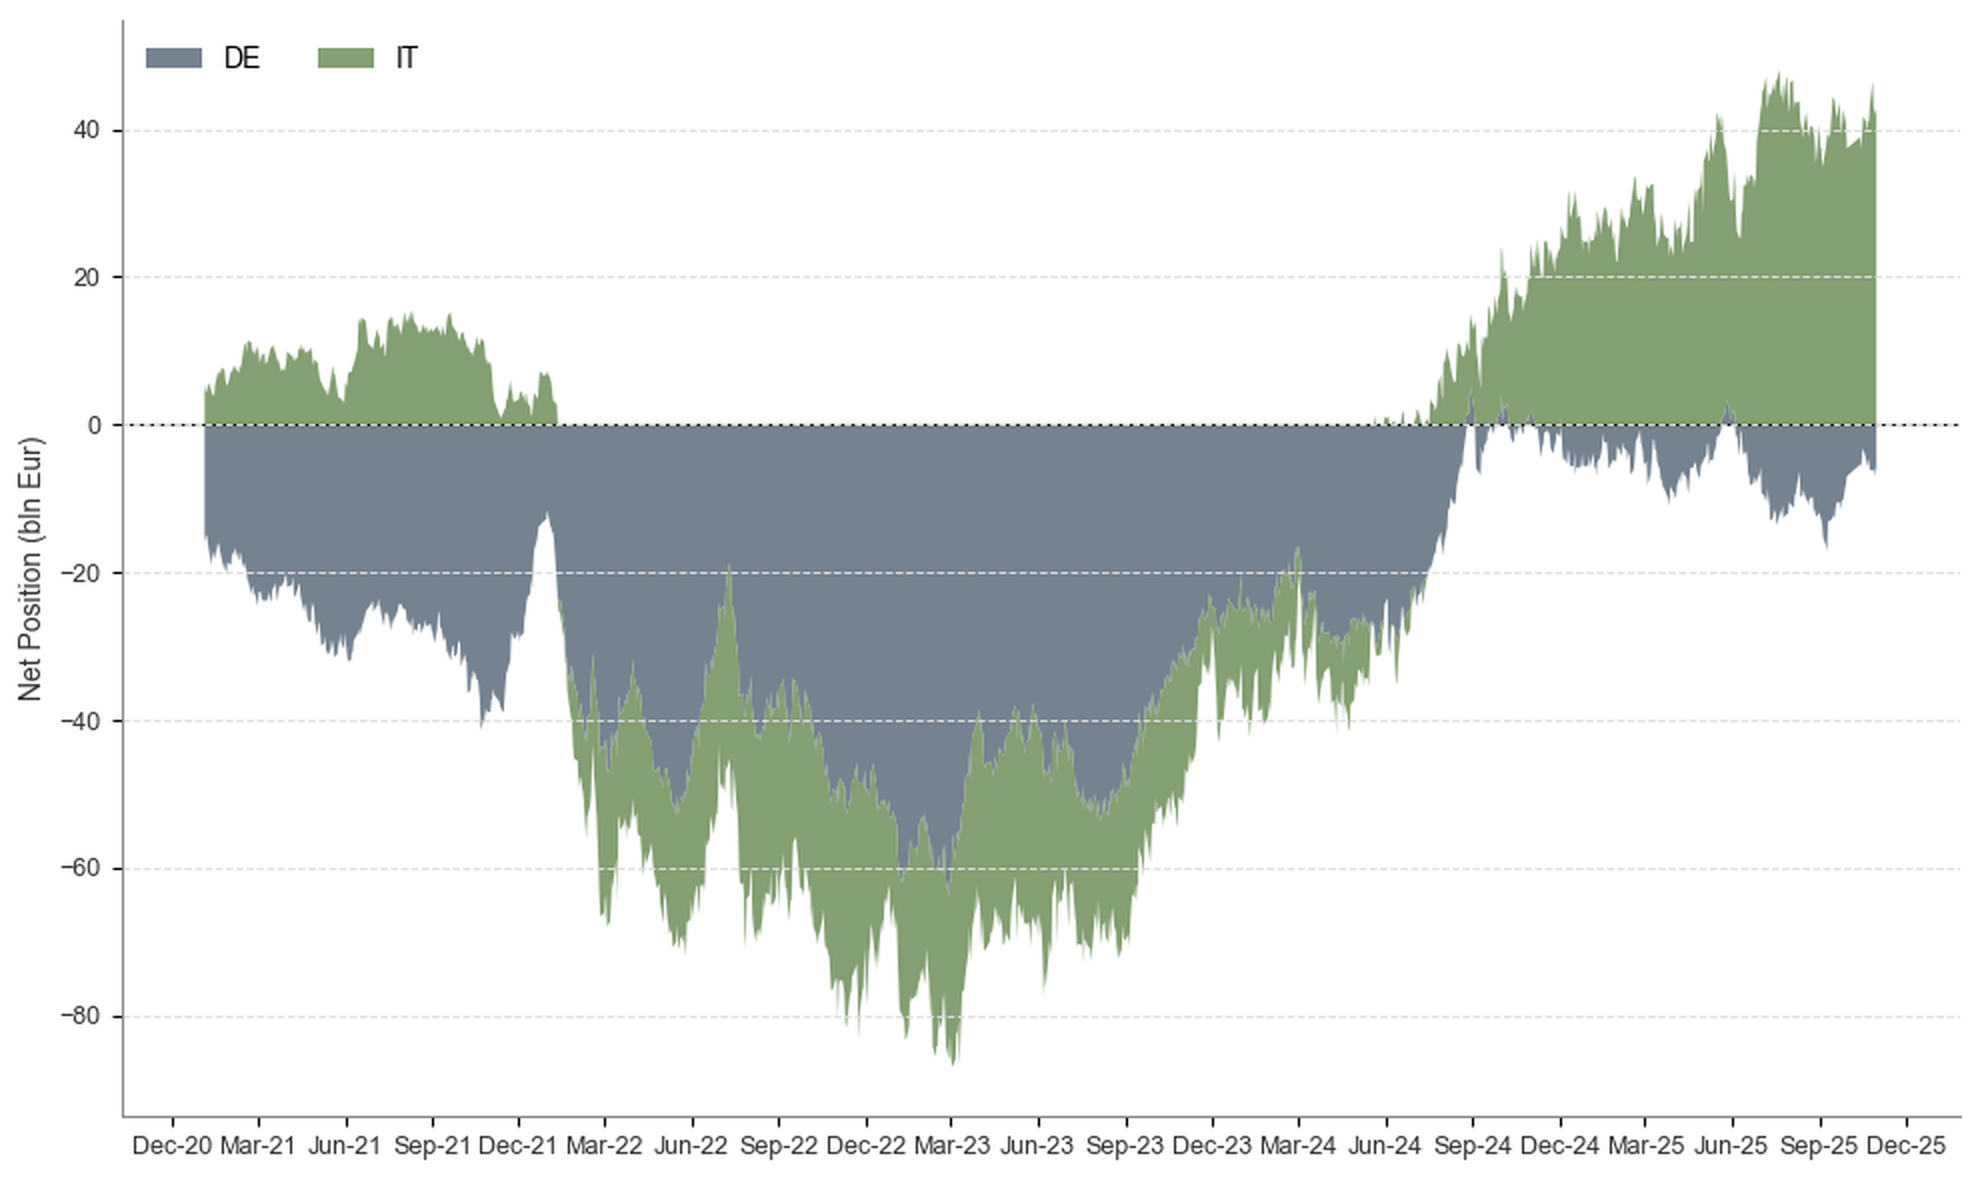
\includegraphics[width=\textwidth]{Figures/motivation_chart.png}
\caption*{\scriptsize \textit{Notes}: Euro outstanding volumes. Positive (negative) values indicate net cash borrowing (lending). \\
    Sample period: 2021-01-01 -- 2025-11-01}
\label{fig:HF_net}
\end{figure}

This variation in positioning underscores the importance of accounting for the direction of hedge fund exposure in the analysis. Since hedge funds adjust their repo positions over time, any empirical framework must take the prevailing state of positioning into account rather than treating their presence as homogeneous.



\subsection{Yield Sensitivity}

This paper argues that the trading activity of hedge funds, as discussed in Section \ref{subsec:trading_regimes}, matters for the sensitivity of a bond's yield. To show evidence of this, Figure \ref{fig:sensitivity} presents a binned scatterplot with the monetary policy shocks on the x-axis and daily yield changes on the y-axis. I then differentiate whether bonds are actively traded by hedge funds. 

\begin{figure}[ht]
\centering
\caption{Yield sensitivity to monetary policy shocks}
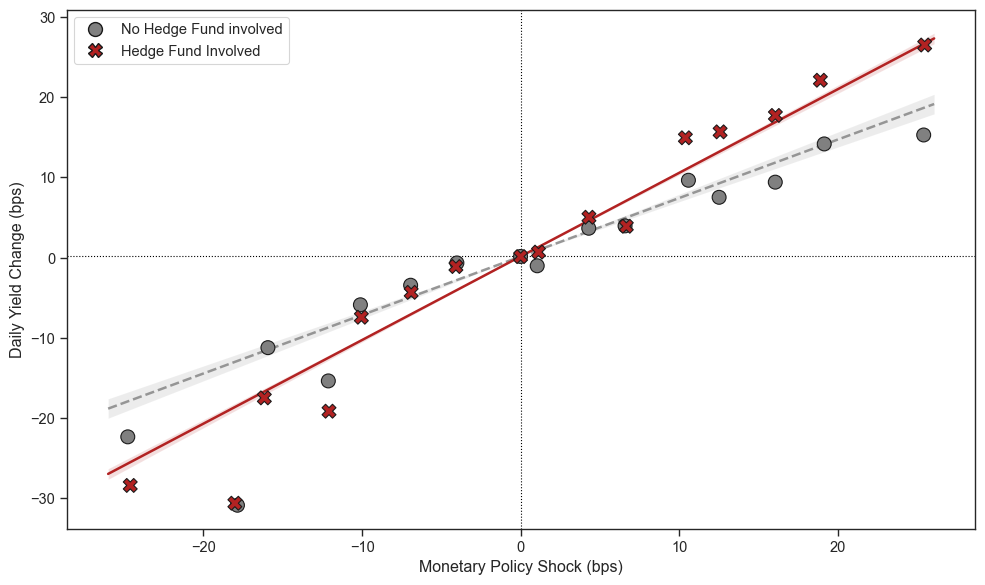
\includegraphics[width=\textwidth]{Figures/shock_reaction_scatterplot.png}
\caption*{\scriptsize \textit{Notes}: Binned scatterplot of daily bond yield changes of German and Italian government bonds against monetary policy shocks. Shocks are defined as the change in the 2-year OIS rate during the ECB monetary event window \citep{altavilla2019}. Yield changes are residualized for bond fixed effects. The sample is winsorized and grouped into equal-width bins. Dots represent the conditional means within each bin. Lines represent linear fits estimated on the underlying bond-level data. \\
Sample period: 2021-01-01 -- 2025-11-01}
\label{fig:sensitivity}
\end{figure}

By definition, the plot results in a positive relationship between the shocks and the yield changes. For bonds that are not traded by hedge funds, the relationship is almost one-to-one, as expected. However, the slope is steeper for bonds that are actively traded by hedge funds. For positive (negative) monetary policy shocks, the yield increase (decrease) is stronger for these bonds. On days where there is no monetary policy shock, which is the center of the graph, there is no difference in the two categories. 

The steeper slope for hedge fund-involved bonds suggests an unconditional amplification effect, which I formally test in Section \ref{sec:empirical_results}.



\section{Leveraged Positioning and Yield Amplification}
\label{sec:mechanism}

In this section, I draw on the literature to explain how leveraged hedge fund positioning amplifies yield sensitivity to shocks. \citet{adrian2014} provide the broader intuition that leveraged intermediaries actively manage their balance sheets in response to the risk environment, expanding positions when constraints are loose and contracting them when constraints bind. The key insight is that the state of the constraint environment can generate symmetric amplification effects with opposite signs of position adjustment depending on the direction of the shock.

I apply this logic to hedge funds, where the constraint environment shifts directly with the value of the collateral backing their positions. A shock that moves prices against a fund's position erodes its capital buffer and tightens its balance sheet constraint, forcing position reduction. A shock that moves prices in favor of the position relaxes the constraint and frees capacity for additional risk-taking. Under constant-leverage targeting, both responses are governed by the same rule of restoring the desired leverage ratio, with the sign of the shock in combination with the position of the fund determining whether positions contract or expand. In both cases, the resulting trading pushes yields further in the direction of the initial shock.

To illustrate the amplification implied by leveraged positioning, I now present a numerical example based on the constraining side of the mechanism. An analogous calculation applies to the relaxing side, with the sign of the position adjustment reversed.

Consider a hedge fund financing a long bond position via the repo market. To hold this position, the fund must post capital equal to the margin requirement $m_i$. Since the repo loan principal is fixed, any exogenous price shock $\Delta P_{i,t}$ is absorbed entirely by the capital buffer. The rate of capital erosion depends on the leverage ratio $1/m_i$:

\begin{equation}
\frac{\Delta E_{i,t}}{E_{i,t-1}} \approx \frac{1}{m_i} \times \frac{\Delta P_{i,t}}{P_{i,t-1}}
\end{equation}

To illustrate the mechanism, I use representative sample moments. The average monetary policy tightening surprise in the sample is approximately 6 basis points. Regarding leverage, the transaction data in Table \ref{tab:summary_stats} shows haircuts averaging 0.24\% for long positions. However, these raw figures may understate the true capital committed by funds due to practices such as portfolio margining, netting, unobserved cash buffers, or hedging activity that reduces the net price exposure relative to the raw repo position \citep{hempel2023, hill2025, hermes2025a}. Therefore, to capture these effects in a stylized way, I assume an effective margin ($m_i$) of 2\%.

Now, consider a hedge fund holding a representative sovereign bond (duration $\approx 7$ years) financed via repo under this 2\% margin assumption. A positive monetary policy shock of 6 basis points induces a price decline of approximately $0.42\%$ ($6\text{ bps} \times 7$). Substituting these values into Equation (1) reveals the magnitude of the margin pressure:

\begin{equation*}
\frac{\Delta E}{E} = \frac{-0.42\%}{2\%} = -21\%
\end{equation*}

Thus, even under this conservative margin assumption, a standard 6 basis point yield move is sufficient to wipe out 21\% of the daily margin buffer.

To restore the margin ratio, the fund must adjust its position. The resulting yield reaction depends on the market's ability to absorb this activity. Let $\lambda$ denote the inverse market elasticity, meaning how much yields react in response to net trading pressure. The additional yield change attributable to the position adjustment can be expressed as:

\begin{equation}
\Delta y_{i,t}^{\text{Amp}} = \lambda \times \left( \frac{\Delta E_{i,t}}{E_{i,t-1}} \times \frac{Q_{i,t-1}}{Q^{\text{Total}}_{i}} \right)
\end{equation}

where the term in parentheses represents the volume of trading normalized by the bond's total amount outstanding.

In this example, I assume the hedge fund sector holds 3\% of the bond's total outstanding volume ($Q_{HF}/Q_{Total} = 0.03$), in line with the conditional sample in Table \ref{tab:summary_stats}. Recall from the previous step that the exogenous price change necessitates adjusting the position by 21\%. Consequently, the aggregate trading pressure amounts to:

\begin{equation*}
\text{Trading pressure} = 21\% \times 3\% = 0.63\% \text{ of outstanding debt}
\end{equation*}

To quantify the yield impact, I choose a market elasticity of $\lambda = 5$ basis points per percentage point of outstanding traded, based on empirical estimates for US and euro area sovereign bond markets \citep{damico2013, eser2016, desantis2020}.

Substituting these parameters into Equation (2) yields the total amplification:

\begin{equation*}
\Delta y^{\text{Amp}} = 5 \text{ bps/pp} \times 0.63 \text{ pp} = \textbf{3.15 bps}
\end{equation*}

Thus, in this example, the position adjustment triggered by a 6 basis point policy surprise generates sufficient trading pressure to amplify the yield reaction by an additional 3.15 basis points. In terms of price, this implies that the position adjustment triggered by the 42 basis point valuation change leads to an additional 22.05 basis point price movement in the direction of the shock.





\section{Empirical Strategy}
\label{sec:empirical_strategy}

\subsection{Specification}
To empirically test the amplification mechanism, I employ a panel regression framework that exploits monetary policy shocks and cross-sectional variation in hedge fund positioning. The strategy is to interact pre-determined hedge fund positions with exogenous price shocks to identify the additional yield sensitivity that arises specifically because hedge funds are active in a given bond.
While the mechanisms explored in Section \ref{sec:mechanism} are general and apply to any event that causes significant price changes, I focus on monetary policy shocks for two reasons. First, since they are identified using high-frequency intraday windows, they are well-defined and exogenous to other daily bond market factors. Second, the shocks generate enough reaction in bond yields to trigger the discussed mechanisms. Figure \ref{fig:exceedance_probability} validates the latter point by plotting the exceedance probability of daily yield changes. The graph shows that shock days display significant fat-tails, meaning that large yield movements are significantly more likely on days with monetary policy announcements.  

\begin{figure}[t]
\centering
\caption{Probability of the Yield Change exceeding a Threshold by Day Type}
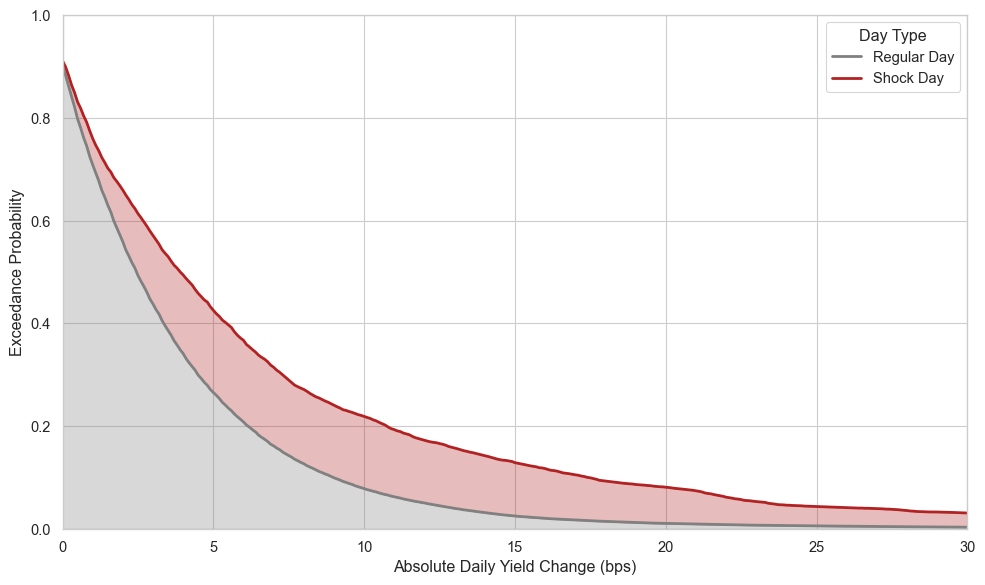
\includegraphics[width=\textwidth]{Figures/exceedance_probability.png}
\caption*{\scriptsize \textit{Notes}: The figure plots the share of observations where the absolute daily yield change in German and Italian government bonds ($|\Delta y|$) is strictly larger than the threshold value displayed on the horizontal axis. The red line represents days with monetary policy announcements, while the gray line represents regular trading days. The shaded region between the curves highlights the excess tail risk generated by monetary policy surprises. \\ Sample period: 2021-01-01 -- 2025-11-01}
\label{fig:exceedance_probability}
\end{figure}


My baseline specification estimates the sensitivity of bond yields to monetary shocks conditional on hedge fund activity. I estimate the following model:

\begin{equation}
\Delta y_{i,t} = \beta_1 (\text{HF}_{i,t-1} \times \text{Shock}_{t}) + \beta_2 \text{HF}_{i,t-1} + \gamma \mathbf{X}_{i,t-1} + \theta_{k} + \varepsilon_{i,t}
\end{equation}
\noindent where the dependent variable, $\Delta y_{i,t}$, is the daily yield change of bond i on day t, and $\theta_{k}$ denotes the fixed effects structure, which varies across specifications as discussed in Section \ref{sec:identification}.

The key explanatory variable is the interaction term $\text{HF}_{i,t-1} \times \text{Shock}_{t}$, where $\text{Shock}_{t}$ represents the monetary policy shock and $\text{HF}_{i,t-1}$ measures hedge fund positioning prior to the shock. I use two complementary definitions for the hedge fund positioning. The first is a binary indicator of hedge fund presence at $t{-}1$. This definition is useful because it captures the extensive margin of hedge fund activity and maps naturally onto a matched-sample design, where each hedge fund bond can be paired with an observationally similar non-hedge fund bond to address selection concerns non-parametrically. The second definition is the average of hedge fund outstanding positions over the prior five trading days scaled by the total amount outstanding, which measures the intensity of hedge fund trading. This continuous measure allows me to test whether the amplification scales with the size of the position, providing evidence on the mechanism. A third measure, the directionality of the books held by the funds active in a bond, requires the full cross section of each fund's positions and is therefore introduced in Section \ref{sec:directionality}.

The coefficient of interest is $\beta_1$, which captures the additional sensitivity of hedge fund-traded bonds to the shock relative to comparable bonds. A positive $\beta_1$ indicates that bonds with hedge fund participation exhibit larger yield changes in response to the same shock. The vector $\mathbf{X}_{i,t-1}$ includes bond-specific controls for the bid-ask spread, the residual maturity, and the status as the CTD bond \citep{pelizzon2025}. Standard errors are two-way clustered at the bond and date level to account for both serial correlation within bonds and cross-sectional dependence across bonds. Section \ref{sec:identification} discusses the identification strategy and the corresponding fixed effects structure in detail.


\subsection{Identification Strategy}
\label{sec:identification}
The primary challenge in identifying the causal impact of hedge fund positioning is the endogeneity of their portfolio choice. Hedge funds do not select assets randomly but rather strategically target liquid bonds, often with special status such as the CTD. Table \ref{tab:hf_selection} documents this pattern directly. In a linear probability model of hedge fund involvement on bond characteristics, a one-standard-deviation tighter bid-ask spread (0.42) is associated with a 23 percentage point higher probability of hedge fund activity, and each additional year of duration raises this probability by 1.3 percentage points. Larger issues and CTD bonds are similarly more likely to attract hedge funds, with coefficients of 3.2 and 7.0 percentage points respectively. A simple correlation between ownership and yield reactions would therefore conflate the effect of leveraged capital with the characteristics that make these bonds attractive to arbitrageurs in the first place.

\begin{table}[t]
\centering
\caption{\textbf{Hedge Fund Bond Selection}}
\footnotesize
\setlength{\tabcolsep}{12pt}
\renewcommand{\arraystretch}{1.1}
\begin{tabular}{l c c c}
\toprule
\textbf{Dependent Variable:} & \multicolumn{3}{c}{\textbf{HF Involvement}} \\
\cmidrule(lr){2-4}
 & (1) & (2) & (3) \\
\midrule
\textit{Bond Characteristics} & & & \\
Duration & 0.012*** & 0.012*** & 0.013*** \\
 & (0.004) & (0.003) & (0.003) \\
Bid-Ask Spread & $-$0.534*** & $-$0.524*** & $-$0.549*** \\
 & (0.039) & (0.038) & (0.040) \\
Amount Issued & 0.030*** & 0.032*** & 0.032*** \\
 & (0.002) & (0.002) & (0.002) \\
CTD Flag & 0.070** & 0.070** & 0.070** \\
 & (0.034) & (0.032) & (0.033) \\
\midrule
Country FE & No & Yes & No \\
Country $\times$ Date FE & No & No & Yes \\
\midrule
Observations & 477,001 & 477,001 & 477,001 \\
R-squared & 0.518 & 0.533 & 0.543 \\
\bottomrule
\end{tabular}
\label{tab:hf_selection}

\vspace{1ex}
\raggedright\scriptsize
\textit{Notes:} Linear probability model where the dependent variable is a binary indicator for offshore hedge fund repo activity in a given bond on a given day. \textit{Duration} is in years. \textit{Bid-Ask Spread} is in euros. \textit{Amount Issued} is the outstanding notional in billion euros. \textit{CTD Flag} is an indicator for cheapest-to-deliver status against an active futures contract. Column (2) adds issuer country fixed effects. Column (3) adds country $\times$ date fixed effects, identifying selection within country-day cells. Standard errors are clustered by business date and bond. *** p$<$0.01, ** p$<$0.05, * p$<$0.10. \\ Sample period: 2021-01-01 -- 2025-11-01
\end{table}

My identification strategy addresses this selection bias by exploiting the unpredictability of monetary policy shocks. The key identifying assumption is that, conditional on fixed effects and bond-specific controls, the interaction between pre-determined hedge fund positioning and the high-frequency surprise is exogenous.\footnote{A residual concern is that pre-existing positioning could be correlated with the realized surprise through a common latent factor. Appendix \ref{subsec:orthogonality} reports an orthogonality test in which aggregate hedge fund positioning on the trading day before each ECB meeting does not predict the realized surprise.} Under this assumption, the coefficient on the interaction term captures the additional yield sensitivity that arises specifically because hedge funds are trading a given bond, rather than the effect of bond characteristics that are correlated with both hedge fund presence and shock sensitivity.

The first feature of the research design supporting this assumption is timing. Because monetary policy shocks are measured over a narrow intraday window around the ECB press conference, they are effectively random relative to positions established at $t{-}1$. Hedge funds cannot predict the precise surprise component of the announcement, ensuring that pre-existing positions are not endogenous to the shock itself. This rules out reverse causality, where hedge funds would adjust their positioning in anticipation of the realized surprise.

However, even without reverse causality, bonds traded by hedge funds may be inherently more volatile and therefore more sensitive to any market-moving event, including monetary policy surprises. Duration is the primary determinant of how strongly a bond's yield reacts to a given rate shock, so comparing a hedge fund bond to a non-hedge fund bond of materially different duration would conflate the amplification effect with mechanical differences in rate sensitivity. A meaningful comparison therefore requires matching bonds on duration within the same market environment. Table \ref{tab:volatility} illustrates this by regressing the absolute daily yield change on a hedge fund presence dummy and its interaction with the absolute shock. The coefficient on HF Involved in Columns (1) and (2) shows that the bonds selected by hedge funds are inherently more volatile. Once bond fixed effects absorb this level in Column (3), the sign flips and becomes marginally negative at $-$0.13 basis points, indicating that within the same bond over time, the days on which hedge funds are active are not the more volatile ones. This pattern is consistent with the unconditional differential reflecting between-bond selection into structurally more volatile bonds, while within-bond timing shows no tendency for hedge fund days to be more turbulent. Column (4) shows that once Date fixed effects are replaced with duration-by-country-by-date fixed effects, the residual differential collapses to an insignificant $-$0.10 basis points. Within cells of bonds with similar duration from the same issuer on the same day, hedge fund bonds are no more volatile than their peers.

\begin{table}[t]
\centering
\caption{\textbf{Bond Volatility and Hedge Fund Presence}}
\footnotesize
\setlength{\tabcolsep}{10pt}
\renewcommand{\arraystretch}{1.1}
\begin{tabular}{l c c c c}
\toprule
\textbf{Dependent Variable:} & \multicolumn{4}{c}{\textbf{$|\Delta$ Bond Yield$|$ (bps)}} \\
\cmidrule(lr){2-5}
 & (1) & (2) & (3) & (4) \\
\midrule
\textit{Main Interaction} & & & & \\
\textbf{HF Involved $\times$ $|$Shock$|$} & \textbf{0.240***} & \textbf{0.241***} & \textbf{0.253***} & \textbf{0.246***} \\
 & (0.071) & (0.071) & (0.069) & (0.058) \\
\addlinespace
\textit{Direct Effects} & & & & \\
$|$Shock$|$ & 0.545*** & 0.541*** &  &  \\
 & (0.102) & (0.102) &  &  \\
HF Involved & 0.459*** & 0.817*** & $-$0.128* & $-$0.098 \\
 & (0.084) & (0.146) & (0.072) & (0.062) \\
\addlinespace
\textit{Controls} & & & & \\
Duration & & $-$0.000 & 0.037 &  \\
 & & (0.013) & (0.060) &  \\
Bid-Ask Spread & & 0.838*** & $-$0.533** & $-$0.525** \\
 & & (0.218) & (0.224) & (0.217) \\
CTD Flag & & 0.413* & 0.504*** & 0.369*** \\
 & & (0.248) & (0.124) & (0.084) \\
\midrule
Bond FE & No & No & Yes & Yes \\
Date FE & No & No & Yes & No \\
Duration $\times$ Date $\times$ Country & No & No & No & Yes \\
\midrule
Observations & 477,001 & 477,001 & 477,001 & 470,852 \\
R-squared & 0.035 & 0.040 & 0.504 & 0.683 \\
\bottomrule
\end{tabular}
\label{tab:volatility}

\vspace{1ex}
\raggedright\scriptsize
\textit{Notes:} The dependent variable is the absolute daily change in bond yield (bps). \textit{HF Involved} is a dummy indicating presence of offshore hedge fund repo activity. $|$Shock$|$ is the absolute value of the 2-year OIS rate change during the ECB monetary event window. In Columns (3) and (4), the $|$Shock$|$ main effect is absorbed by the fixed effects. Column (4) replaces Date FE with Duration $\times$ Date $\times$ Country FE, which compares bonds with similar duration from the same issuer country on the same day. Standard errors are clustered by business date and bond. *** p$<$0.01, ** p$<$0.05, * p$<$0.10. \\ Sample period: 2021-01-01 -- 2025-11-01
\end{table}

Based on this evidence, the preferred specification for the analyses throughout the paper includes duration-by-country-by-date fixed effects. This structure absorbs the aggregate shock and any differential volatility across duration-country-date cells, so identification comes exclusively from within-cell variation in hedge fund positioning. 

While the duration-by-country-by-date fixed effects absorb within-cell differences in average bond characteristics, and thereby address the concern about increased volatility, there could still be concerns that it does not eliminate residual heterogeneity among bonds within the same cell, particularly along the liquidity dimension that most strongly predicts hedge fund selection as shown in Table \ref{tab:hf_selection}. For that reason, I use a matched approach in the binary case, which pairs each hedge fund bond on a given day with the single non-hedge fund bond in the same duration-country-date cell that is closest in terms of bid-ask spread. The baseline regression is then run on this matched sample with pair fixed effects, so that identification comes from comparing each hedge fund bond only to its most similar non-hedge fund counterpart. This design makes the comparison group transparent and eliminates residual differences in observable characteristics without imposing a functional form on how these characteristics relate to yield sensitivity.

The intensity analysis provides an additional identification argument beyond the binary case. If the amplification were driven solely by unobserved bond characteristics, within-bond variation in the size of the position should not predict the yield reaction, since bond fixed effects absorb any time-invariant sensitivity. However, the leveraged-position mechanism implies that larger positions trigger larger forced sales, so the amplification should scale with the size of the exposure within the same bond over time. Testing the continuous intensity measure in addition to the binary indicator therefore provides a test of the mechanism that is difficult to reconcile with a selection story.

Finally, a separate but related concern is that the amplification could reflect not the leveraged positioning of hedge funds themselves but the behavior of the dealers that intermediate their trades. Because this concern cannot be addressed within the bond-date panel used in the main specifications, I restructure the panel at the dealer-bond-date level and use progressively tighter dealer fixed effects structures to hold dealer behavior constant on each day.



\section{Empirical Results and Discussion}
\label{sec:empirical_results}

\subsection{Hedge Fund Presence}
\label{subsec:baseline}
I begin by examining whether the mere presence of hedge funds creates a differential sensitivity to monetary policy. I estimate the baseline specification using a binary indicator for hedge fund activity:

\begin{equation}
    \Delta y_{i,t} = \theta_{k} + \beta (HF\_Involved_{i,t-1} \times Shock_{t}) + \gamma \mathbf{X}_{i,t} + \varepsilon_{i,t}
\end{equation}

where $HF\_Involved_{i,t-1}$ is a dummy variable equal to one if bond $i$ has active offshore hedge fund repo positions on day $t-1$. The variable $\text{Shock}_{t}$ represents the high-frequency adjustment in 2-year OIS rates \citep{altavilla2019}. $\theta_{k}$ denotes the fixed effects structure, which varies across specifications.

The vector of controls $\mathbf{X}_{i,t-1}$ includes duration, bid-ask spreads, and the Cheapest-to-Deliver (CTD) status. Following \citet{pelizzon2025}, I identify the CTD bond using delivery data from Eurex, assuming the delivered bond acts as the CTD throughout the futures contract life.

\begin{table}[t]
\centering
\caption{\textbf{Hedge Fund Amplification}}
\footnotesize
\setlength{\tabcolsep}{9pt}
\renewcommand{\arraystretch}{1.1}
\begin{tabular}{l c c c c c}
\toprule
\textbf{Dependent Variable:} & \multicolumn{5}{c}{\textbf{$\Delta$ Bond Yield (bps)}} \\
\cmidrule(lr){2-6}
 & (1) & (2) & (3) & (4) & (5) \\
\midrule
\textit{Main Interaction} & & & & & \\
\textbf{HF Involved $\times$ Shock} & \textbf{0.288***} & \textbf{0.288***} & \textbf{0.287***} & \textbf{0.291***} & \textbf{0.304***} \\
 & (0.072) & (0.072) & (0.073) & (0.062) & (0.055) \\
\addlinespace
\textit{Direct Effects} & & & & & \\
Shock & 0.757*** & 0.757*** &  &  &  \\
 & (0.123) & (0.123) &  &  &  \\
HF Involved & 0.083** & 0.062 & $-$0.000 & $-$0.022 & $-$0.002 \\
 & (0.037) & (0.059) & (0.043) & (0.038) & (0.025) \\
\addlinespace
\textit{Controls} & & & & & \\
Duration & & 0.003 & 0.037 &  &  \\
 & & (0.005) & (0.042) &  &  \\
Bid-Ask Spread & & $-$0.034 & $-$0.239*** & $-$0.257*** &  \\
 & & (0.086) & (0.085) & (0.075) &  \\
CTD Flag & & 0.157* & 0.033 & 0.010 & 0.003 \\
 & & (0.094) & (0.041) & (0.028) & (0.047) \\
\midrule
Bond FE & No & No & Yes & Yes & No \\
Date FE & No & No & Yes & No & No \\
Duration $\times$ Date $\times$ Country FE & No & No & No & Yes & No \\
Matched Pair FE & No & No & No & No & Yes \\
\midrule
Observations & 477,001 & 477,001 & 477,001 & 470,852 & 481,746 \\
R-squared & 0.033 & 0.033 & 0.569 & 0.737 & 0.842 \\
\bottomrule
\end{tabular}
\label{tab:baseline}

\vspace{1ex}
\raggedright\scriptsize
\textit{Notes:} The dependent variable is the daily change in bond yield (bps). \textit{HF Involved} is a dummy indicating presence of offshore hedge fund repo activity. \textit{Shock} is the 2-year OIS rate change during the ECB monetary event window. In Columns (3) and (4), the Shock main effect is absorbed by the fixed effects. Column (4) adds bond and Duration $\times$ Date $\times$ Country fixed effects. Column (5) presents the matched-sample estimation. Standard errors are clustered by business date and bond in Columns (1)–(4), and by Duration $\times$ Date $\times$ Country and non-HF bond in Column (5). *** p$<$0.01, ** p$<$0.05, * p$<$0.10. \\ Sample period: 2021-01-01 -- 2025-11-01
\end{table}

Table \ref{tab:baseline} presents the estimation results. Across all five specifications, the interaction coefficient of interest ($\beta$) is positive, statistically significant at the 1\% level, and remarkably stable, ranging from 0.288 to 0.304.

Column (1) reports the unconditional correlation. The interaction coefficient of 0.288 implies that for every 1 basis point increase in the benchmark yield shock, bonds with hedge fund presence experience an additional yield increase of approximately 0.3 basis points. Column (2) introduces bond-specific controls which barely impacts the magnitude of the coefficient. This suggests that the excess sensitivity is not merely a proxy for a liquidity premium or the special status of the assets. Column (3) absorbs time-invariant bond characteristics (Bond FE) and aggregate daily shocks (Time FE). Even within this set-up, the interaction coefficient remains robust at 0.287. Because the bond fixed effects absorb all time-invariant characteristics, identification here comes from comparing the same bond during periods when hedge funds are active to periods when they are not, rather than from comparing different bonds to each other.

Column (4) tightens the identification further by replacing the Date fixed effects with Duration $\times$ Country $\times$ Date fixed effects. This structure compares bonds with similar duration from the same issuer country on the same day, absorbing both the aggregate shock and any differential rate sensitivity that mechanically arises from differences in duration. Identification therefore relies exclusively on within-cell variation in hedge fund positioning among bonds that are otherwise comparable in their exposure to the shock. As shown in Section \ref{sec:empirical_strategy}, hedge fund bonds are not more volatile than their peers within these cells on average, making this the appropriate comparison group for isolating the shock-conditional amplification. Under this tighter specification, the interaction coefficient increases slightly to 0.291 and remains significant at the 1\% level, while the direct effect of HF Involved remains insignificant. Together, these results indicate that hedge fund bonds are not significantly different from comparable non-hedge fund bonds in normal times, but become significantly more sensitive precisely when a shock interacts with the leveraged positioning.

Column (5) presents the matched-sample estimation. While the duration-country-date fixed effects in Column (4) ensure that hedge fund bonds are compared to peers with similar rate sensitivity, they do not eliminate residual heterogeneity within cells, particularly along the liquidity dimension that most strongly predicts hedge fund selection (Table \ref{tab:hf_selection}). A matched-sample design addresses this concern by making the comparison group fully transparent and by eliminating residual differences in observable characteristics non-parametrically, without imposing a functional form on how these characteristics relate to yield sensitivity. Specifically, I pair each hedge fund bond on a given day with the single non-hedge fund bond in the same duration-country-date cell that is closest in terms of bid-ask spread, and estimate the regression on this matched sample with pair fixed effects. Each hedge fund bond is therefore benchmarked only against its most similar non-hedge fund counterpart. Under this design, the interaction coefficient rises slightly to 0.304 and remains significant at the 1\% level. The stability of the estimate across the progressively tighter specifications indicates that the amplification is not driven by selection on observable bond characteristics, but reflects the impact of leveraged positioning itself.

The estimated amplification is economically substantial. To put the coefficients into perspective, consider the impact of an average six basis point monetary policy tightening surprise. The baseline reaction of a typical bond (captured by the direct Shock coefficient in Column 1 or 2) implies a yield change of approximately $0.757 \times 6 \text{ bps} \approx 4.54 \text{ bps}$.

For a bond with hedge fund participation, the interaction term adds an excess movement of $0.288 \times 6 \text{ bps} \approx 1.73 \text{ bps}$. Consequently, the total yield reaction for hedge fund-held bonds rises to 6.27 basis points. This implies that the trading of hedge funds in specific bonds accounts for approximately 28\% of the total yield movement on shock days. In other words, more than one-quarter of the price action in these bonds is associated not with the fundamental news, but with the type of entity trading them. \footnote{Because hedge funds may also hold leveraged positions through instruments beyond the repo market, a natural concern is that the estimated amplification reflects unobserved derivative exposure transmitting to cash yields through the cheapest-to-deliver linkage. Appendix \ref{subsec:ctd} re-estimates the main specifications on the subsample of non-CTD bonds and finds nearly identical coefficients.}


\begin{figure}[t]
    \centering
    \caption{Persistence of the amplification}
    \begin{subfigure}[t]{0.49\textwidth}
        \centering
        \caption{Matched differential}
        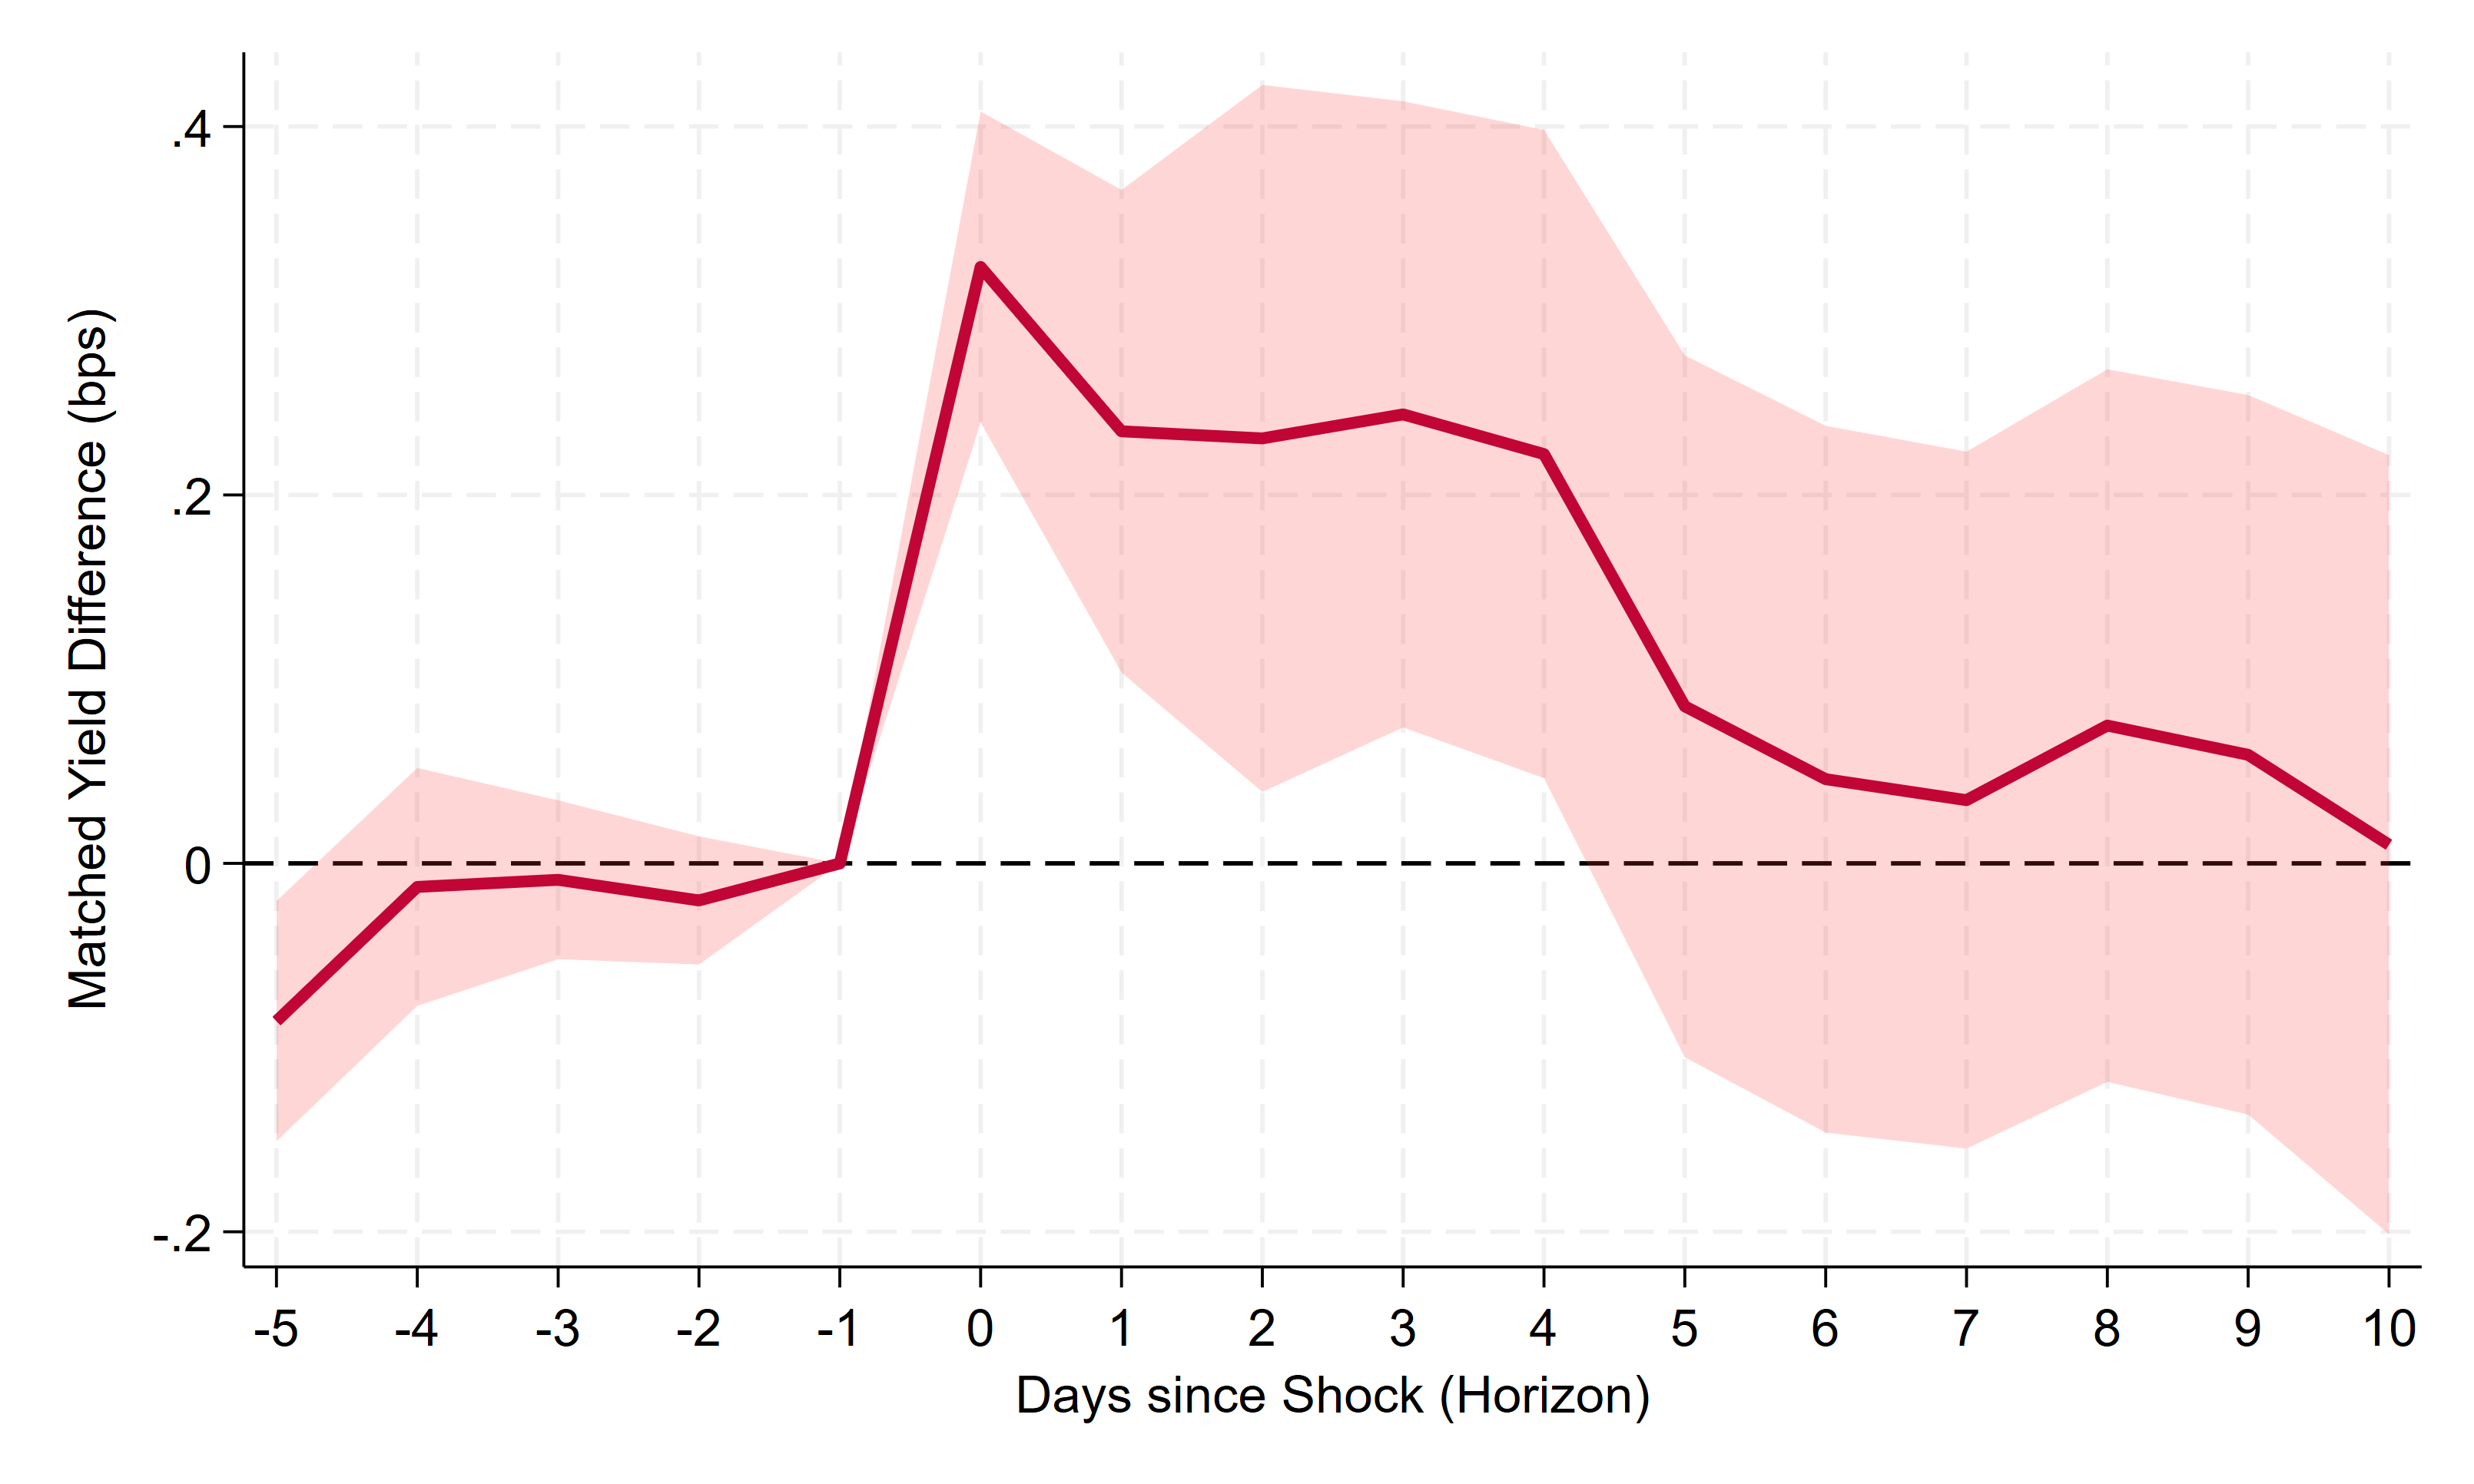
\includegraphics[width=\textwidth]{Figures/IR_baseline.png}
        \label{fig:baseline_persistence}
    \end{subfigure}
    \hfill
    \begin{subfigure}[t]{0.49\textwidth}
        \centering
        \caption{Level decomposition}
        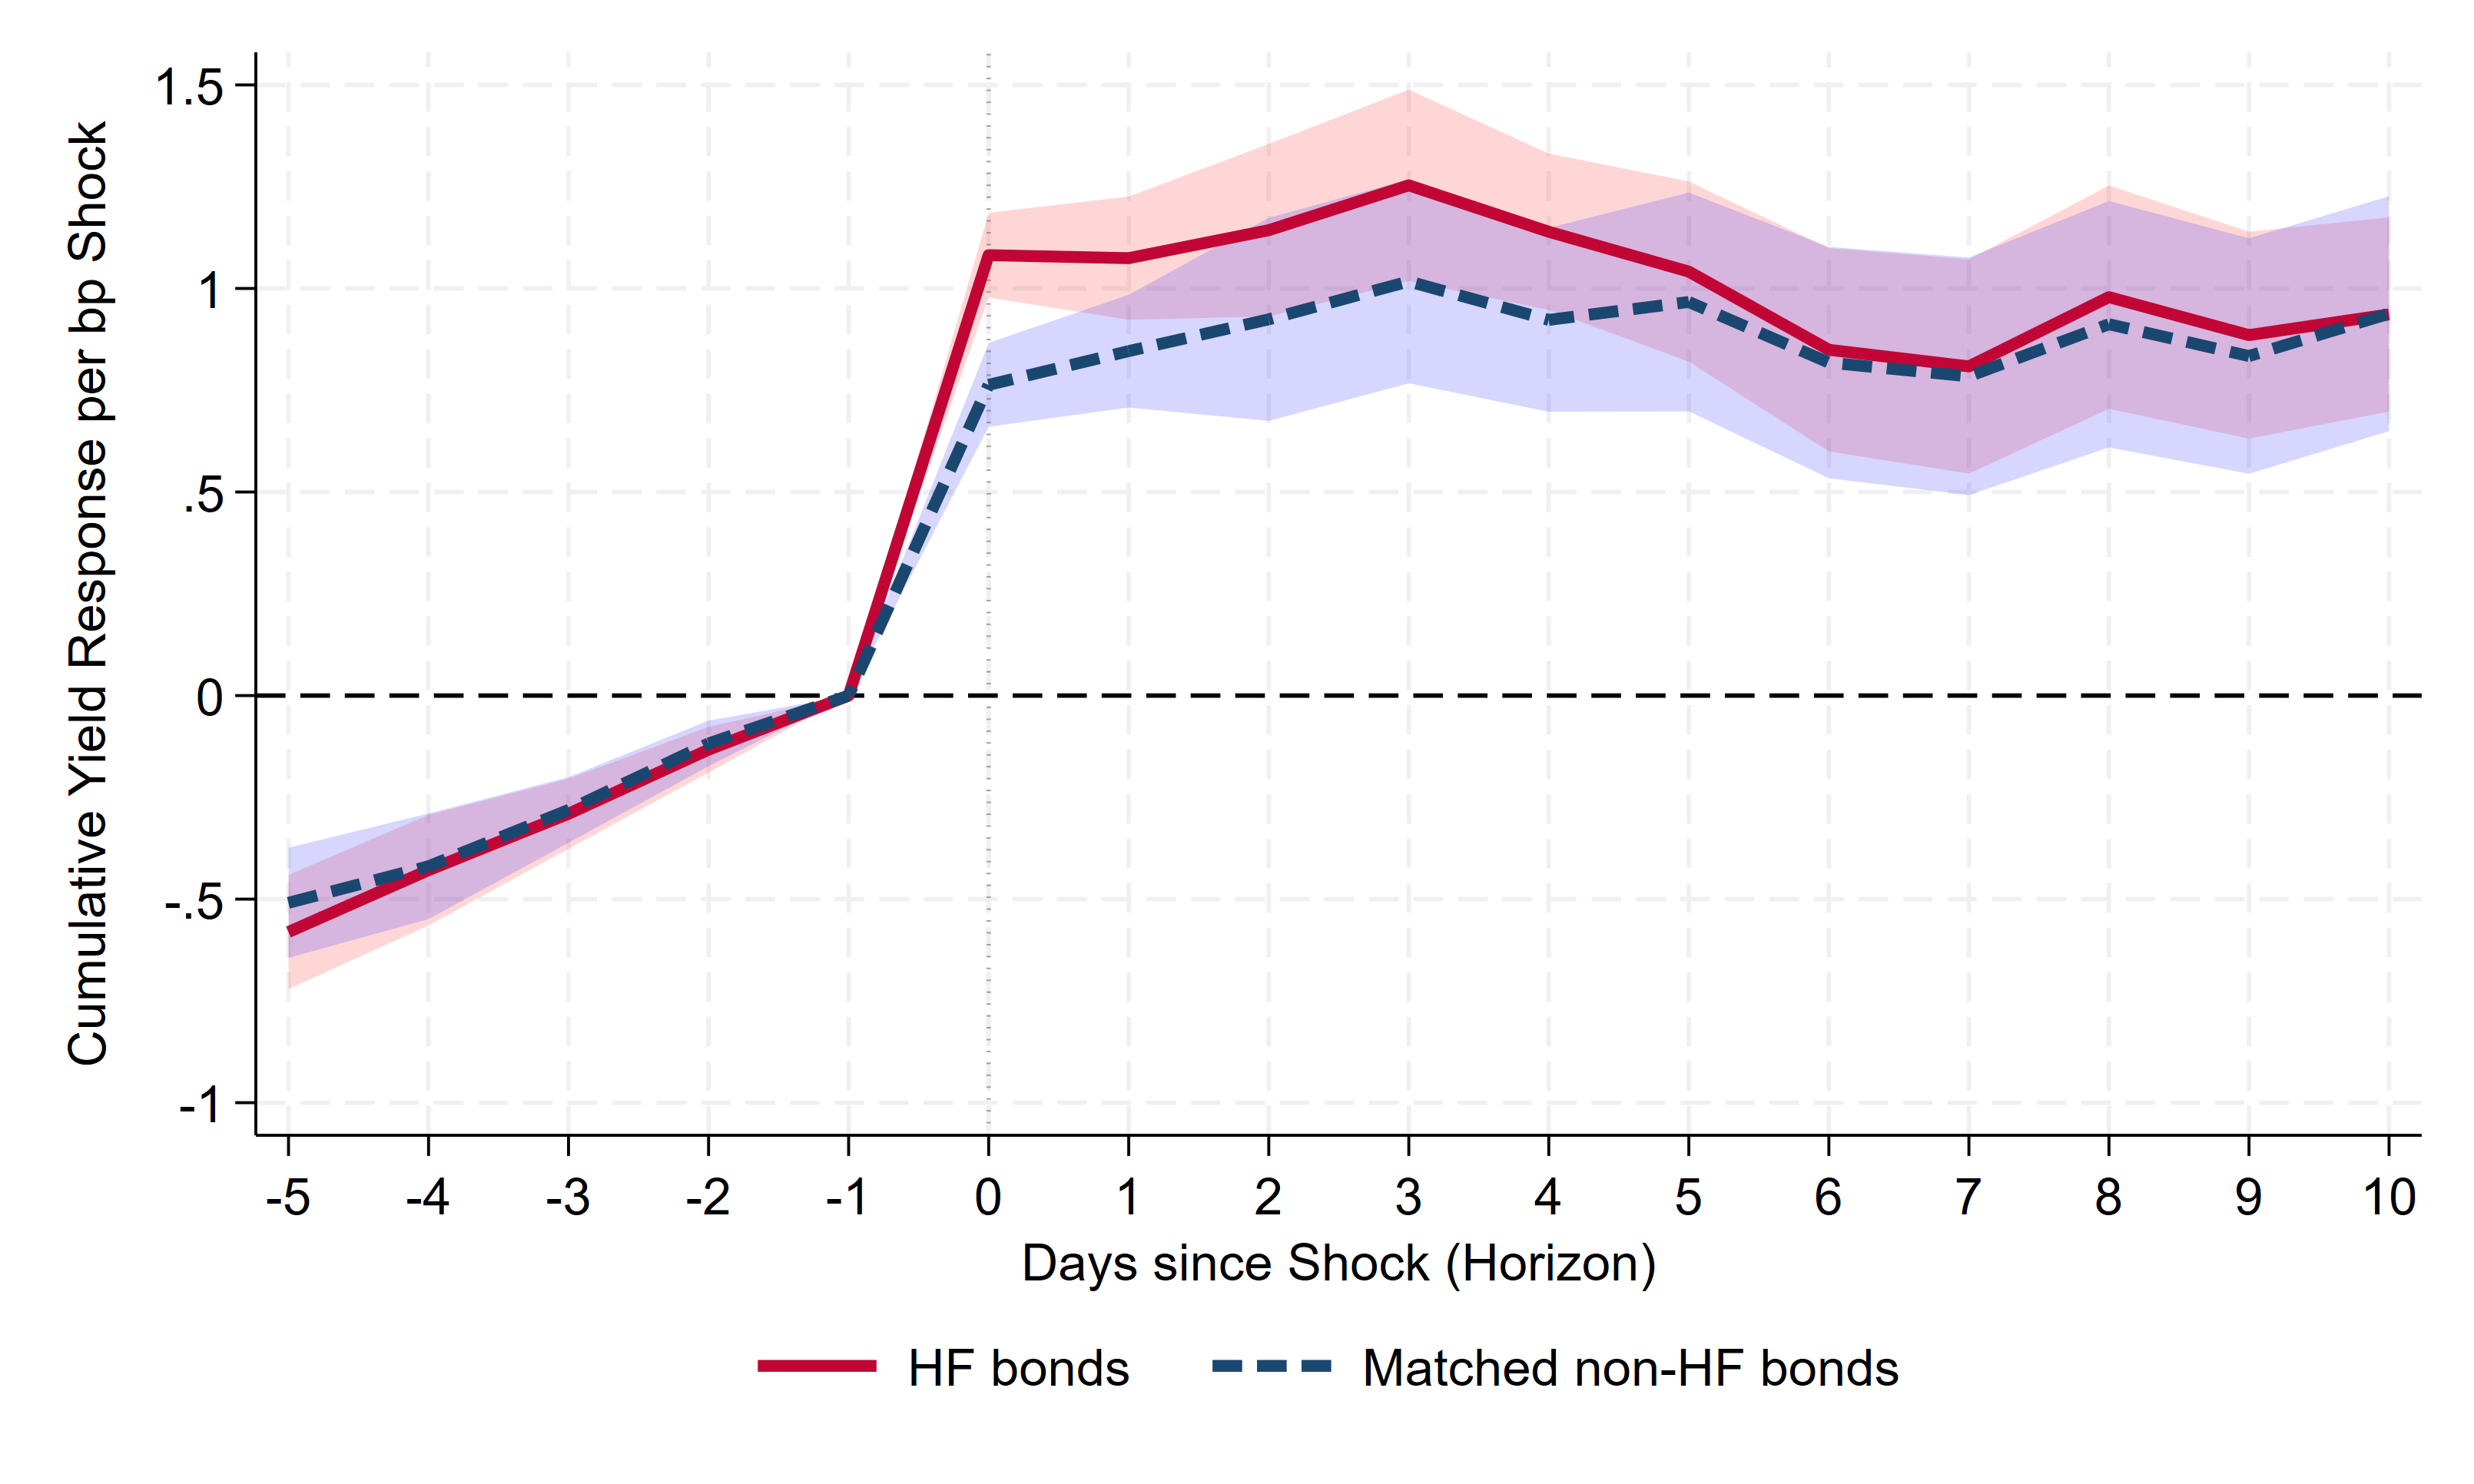
\includegraphics[width=\textwidth]{Figures/IR_baseline_decomposition.png}
        \label{fig:baseline_persistence_decomp}
    \end{subfigure}
    \caption*{\scriptsize \textit{Notes:} Panel (a) plots the estimated interaction coefficients $\beta_h$ from regressions of cumulative yield changes ($\Delta y_{t-1 \rightarrow t+h}$) on the interaction between the HF presence dummy and monetary policy shocks, representing the differential yield response (in bps) of HF-involved bonds relative to non-HF bonds. Panel (b) decomposes this differential by plotting the cumulative yield response per basis point of shock separately for HF-involved bonds and their matched non-HF counterparts. Both panels are based on the matched sample set-up. Shaded areas denote 90\% confidence intervals clustered by business date and bond. \\ Sample period: 2021-01-01 -- 2025-11-01}
\end{figure}

To examine the persistence of this amplification, I estimate the impulse response function using the local projection methodology of \citet{jorda2005}. The local projections are based on the matched-sample design from Column (5) of Table \ref{tab:baseline}, with cumulative yield changes regressed on the interaction between the HF presence dummy and monetary policy shocks. Figure \ref{fig:baseline_persistence} plots the estimated coefficients $\beta_h$ over a window from $h=-5$ to $h=10$ trading days around the shock.

Figure \ref{fig:baseline_persistence} provides two insights. First, the pre-shock coefficients are flat and insignificant, which speaks to the concern about selection bias by providing evidence that hedge fund-involved bonds and their matched counterparts do not differ significantly in the days leading up to the announcement. Second, the divergence appears immediately on the impact day, remains statistically significant for approximately four trading days, and then reverts back toward zero by the end of the horizon. Figure \ref{fig:baseline_persistence_decomp} decomposes this differential into the underlying level responses and shows that both series converge toward a common terminal value of slightly below one basis point per basis point of shock. The convergence in levels is consistent with theories of slow-moving capital in which the market requires time to absorb the imbalance generated by leveraged trading \citep{duffie2010, mitchell2007}.

If hedge funds were primarily correcting mispricings, their trading would push yields toward fundamental values and the effect would persist. Instead, Figure \ref{fig:baseline_persistence_decomp} shows that HF-involved bonds overshoot the common terminal value during the first days after the shock before reverting back, which is evidence of non-fundamental liquidity shocks \citep{coval2007}.

A complementary test of the overshooting interpretation comes from decomposing the shock itself rather than the response. Using the sign restrictions of \citet{jarocinski2020}, each ECB surprise can be classified into a pure monetary component and a central bank information component based on the comovement of yields and equity prices within the event window. Under the price-discovery alternative, the HF amplification should be at least as strong for information-driven surprises, since that is the component where the ECB reveals new macroeconomic information that informed investors would process faster. Table \ref{tab:jk} reports the HF amplification separately for each component. The interaction coefficient is 0.377 for pure monetary surprises and 0.113 for information surprises. The amplification is therefore concentrated in the component of the surprise that does not reflect new fundamental information, which is the opposite of what a price-discovery story would predict.

Taken together, the level decomposition in Figure \ref{fig:baseline_persistence_decomp} and the shock decomposition in Table \ref{tab:jk} point to the same conclusion through independent channels. HF bonds overshoot their own terminal level during the first days after the shock, and the amplification is concentrated in pure monetary rather than information-driven surprises. Hedge fund activity moves prices away from fundamentals in the short run, and the dislocation is only gradually undone as other capital arrives. Within the sovereign bond market studied here, the evidence is therefore more consistent with the amplification view of leveraged non-bank trading than with the price-discovery view.

\begin{table}[t]
\centering
\caption{\textbf{Hedge Fund Amplification by Shock Component}}
\footnotesize
\setlength{\tabcolsep}{10pt}
\renewcommand{\arraystretch}{1.1}
\begin{tabular}{l c c}
\toprule
\textbf{Dependent Variable:} & \multicolumn{2}{c}{\textbf{$\Delta$ Bond Yield (bps)}} \\
\cmidrule(lr){2-3}
 & (1) Monetary & (2) Information \\
\midrule
\textbf{HF Involved $\times$ Shock} & \textbf{0.377***} & \textbf{0.113***} \\
 & (0.139) & (0.042) \\
\addlinespace
HF Involved & $-$0.019 & $-$0.026 \\
 & (0.036) & (0.037) \\
\midrule
Controls & Yes & Yes \\
Bond FE & Yes & Yes \\
Duration $\times$ Date $\times$ Country FE & Yes & Yes \\
\midrule
Observations & 470,852 & 470,852 \\
R-squared & 0.737 & 0.737 \\
\bottomrule
\end{tabular}
\label{tab:jk}

\vspace{1ex}
\begin{minipage}{\textwidth}
\scriptsize
\textit{Notes:} The dependent variable is the daily change in bond yield (bps). \textit{HF Involved} is a dummy indicating presence of offshore hedge fund repo activity. The shock in Column (1) is the pure monetary component and in Column (2) the central bank information component of the ECB surprise, decomposed using the sign restrictions of \citet{jarocinski2020}. Both specifications include bond fixed effects, duration $\times$ date $\times$ country fixed effects, and bond-level controls for bid-ask spread and CTD status. The Shock main effect is absorbed by the fixed effects. A Wald test of equality between the two interaction coefficients rejects the null ($p = 0.065$). Standard errors are clustered by business date and bond. *** p$<$0.01, ** p$<$0.05, * p$<$0.10. \\ Sample period: 2021-01-01 -- 2025-11-01
\end{minipage}
\end{table}



A remaining concern is that the documented amplification could reflect not the leveraged positioning of hedge funds themselves but the behavior of the dealers that intermediate their trades. Dealers may adjust inventory, hedge exposure, or update pricing more aggressively on shock days in the specific bonds where they maintain active hedge fund relationships, and these adjustments could generate yield movements that would appear in the data as an HF-associated effect even if hedge funds themselves were passive. This concern is distinct from the role of dealer intermediation capacity in transmitting the flow, which is a complement to the leveraged positioning channel rather than a substitute for it. The question I address here is whether the trigger of the amplification lies with the dealer rather than with the hedge fund.

To address this concern, I restructure the panel at the dealer-bond-date level and re-estimate the baseline specification with progressively tighter dealer-side fixed effects. The unit of observation is now a dealer-bond-date, and the panel is balanced so that dealer-bond-days without active intermediation enter with zero positions. This structure allows me to absorb dealer behavior at the day level and identify the amplification from variation across bonds traded by the same dealer on the same day.


\begin{table}[t]
\centering
\caption{\textbf{Amplification Within Dealer Behavior}}
\footnotesize
\setlength{\tabcolsep}{8pt}
\renewcommand{\arraystretch}{1.1}
\begin{tabular}{l c c c c}
\toprule
\textbf{Dependent Variable:} & \multicolumn{4}{c}{\textbf{$\Delta$ Bond Yield (bps)}} \\
\cmidrule(lr){2-5}
 & (1) & (2) & (3) & (4) \\
\midrule
\textit{Main Interaction} & & & & \\
\textbf{HF Involved $\times$ Shock} & \textbf{0.271***} & \textbf{0.294***} & \textbf{0.248***} & \textbf{0.250***} \\
 & (0.057) & (0.056) & (0.051) & (0.054) \\
\addlinespace
\textit{Direct Effect} & & & & \\
HF Involved & 0.006 & 0.007* & 0.001 & 0.001 \\
 & (0.004) & (0.004) & (0.004) & (0.007) \\
\addlinespace
\textit{Triple Interaction} & & & & \\
HF Involved $\times$ Shock $\times$ $\Delta$CDS & & & & 0.000 \\
 & & & & (0.003) \\
HF Involved $\times$ $\Delta$CDS & & & & $-$0.003 \\
 & & & & (0.007) \\
\addlinespace
\textit{Controls} & & & & \\
Duration & 0.035 & 0.053 & 0.077* & 0.076* \\
 & (0.043) & (0.040) & (0.037) & (0.037) \\
Bid-Ask Spread & $-$0.257*** & $-$0.235*** & $-$0.270*** & $-$0.274*** \\
 & (0.088) & (0.080) & (0.077) & (0.077) \\
CTD Flag & 0.042 & 0.051 & 0.027 & 0.026 \\
 & (0.041) & (0.040) & (0.028) & (0.028) \\
\midrule
Bond FE & Yes & Yes & Yes & Yes \\
Dealer $\times$ Date FE & Yes & No & No & No \\
Dealer $\times$ Date $\times$ Country FE & No & Yes & No & No \\
Dealer $\times$ Date $\times$ Dur. FE & No & No & Yes & Yes \\
\midrule
Observations & 8,422,704 & 8,422,704 & 8,313,714 & 8,289,774 \\
R-squared & 0.570 & 0.619 & 0.738 & 0.738 \\
\bottomrule
\end{tabular}
\label{tab:dealer_robustness}
\vspace{1ex}
\begin{minipage}{\textwidth}
\scriptsize
\textit{Notes:} The dependent variable is the daily change in bond yield (bps). The unit of observation is dealer-bond-date and the panel is balanced, with zero positions retained for dealer-bond-days without active repo intermediation. HF Involved is a dummy indicating that the dealer had an outstanding repo position with a hedge fund counterparty in the given bond over the prior five trading days. Hedge funds are offshore investment funds domiciled in the Cayman Islands. Shock is the 2-year OIS rate change during the ECB monetary event window. $\Delta$CDS$_{t-1}$ is the five-day change in the dealer's own CDS spread measured as of the trading day before the shock. The Shock main effect is absorbed by the Dealer $\times$ Date fixed effects across all specifications. Column (1) absorbs any time-varying dealer-level behavior on each day. Column (2) additionally holds the issuer country constant within each dealer-day cell. Columns (3) and (4) tighten this further by additionally controlling for duration, so that identification comes from comparing bonds with similar rate sensitivity traded by the same dealer on the same day. Column (4) adds the triple interaction with the dealer's own five-day CDS change to test whether the amplification scales with dealer stress. Standard errors are clustered by dealer, business date, and bond. *** p$<$0.01, ** p$<$0.05, * p$<$0.10. \\ Sample period: 2021-01-01 -- 2025-11-01
\end{minipage}
\end{table}

Table \ref{tab:dealer_robustness} presents the results. Column (1) absorbs dealer-by-date fixed effects, which hold constant any time-varying behavior of a given dealer on a given day, including inventory management, funding conditions, hedging activity, and idiosyncratic risk appetite. Identification therefore comes exclusively from comparing bonds traded by the same dealer on the same day. The HF interaction coefficient is 0.271 and significant at the 1\% level. Columns (2) and (3) progressively tighten this structure by additionally holding constant the issuer country and the duration of the bond within each dealer-day cell, so that the comparison group consists of bonds with similar rate sensitivity traded by the same dealer on the same day. The coefficient remains positive and significant at the 1\% level across both specifications, ranging from 0.248 to 0.294.

Column (4) adds a triple interaction with the five-day change in the dealer's own CDS spread, measured as of the trading day before the shock. This tests whether the amplification scales with dealer-specific stress, as a dealer-driven alternative would predict. The triple interaction is economically and statistically indistinguishable from zero, and the HF interaction coefficient is unchanged at 0.250. Dealer stress, as captured by the dealer's own credit spread, does not contribute to the amplification.

Taken together, these results indicate that the amplification documented in this section is not a byproduct of dealer behavior. Within the same dealer on the same day, bonds where hedge funds are positioned react more strongly to monetary policy shocks than otherwise comparable bonds, and this differential does not scale with the dealer's own stress. While dealer intermediation is necessary for the flow to reach the market, the trigger of the amplification operates through the leveraged positioning of the hedge funds themselves rather than through the response of the dealers that face them.


\subsection{Hedge Fund Intensity}
In this section, I extend the analysis beyond the binary presence of hedge funds to examine whether the size of the position amplifies the yield reaction. As outlined in the conceptual framework, the price impact of the position adjustment should depend on the volume of trading relative to the total market depth.

To capture this, I construct a continuous measure called Hedge Fund Intensity. For each bond-day, I calculate the average absolute net position over the previous five trading days and scale it by the bond's total amount outstanding. This ratio directly measures the percentage of a specific bond held by these offshore hedge funds. I then take the natural log of one plus this ratio. The economic rationale for the log specification is that small trading pressures can be absorbed by dealer inventory and standing arbitrage capital without measurable price impact, while larger pressures exhaust this absorption capacity and begin to move yields, with each additional unit of pressure mattering less once the dislocation is underway. A log transformation captures this concavity in a single functional form. Appendix \ref{subsec:categorical} verifies that the relationship is monotone across discrete intensity buckets.

\begin{table}[t]
\centering
\caption{\textbf{Hedge Fund Intensity}}
\footnotesize
\setlength{\tabcolsep}{10pt}
\renewcommand{\arraystretch}{1.1}
\begin{tabular}{l c c c c}
\toprule
\textbf{Dependent Variable:} & \multicolumn{4}{c}{\textbf{$\Delta$ Bond Yield (bps)}} \\
\cmidrule(lr){2-5}
 & (1) & (2) & (3) & (4) \\
\midrule
\textit{Main Interaction} & & & & \\
\textbf{Log HF Intensity $\times$ Shock} & \textbf{0.166***} & \textbf{0.165***} & \textbf{0.167***} & \textbf{0.164***} \\
 & (0.035) & (0.035) & (0.036) & (0.032) \\
\addlinespace
\textit{Direct Effects} & & & & \\
Shock & 0.811*** & 0.811*** &  &  \\
 & (0.118) & (0.118) &  &  \\
Log HF Intensity & 0.008 & $-$0.020 & $-$0.009 & $-$0.011 \\
 & (0.024) & (0.033) & (0.025) & (0.017) \\
\addlinespace
\textit{Controls} & & & & \\
Duration & & 0.005 & 0.038 &  \\
 & & (0.004) & (0.042) &  \\
Bid-Ask Spread & & $-$0.101 & $-$0.240*** & $-$0.259*** \\
 & & (0.068) & (0.085) & (0.075) \\
CTD Flag & & 0.189* & 0.033 & 0.010 \\
 & & (0.100) & (0.040) & (0.028) \\
\midrule
Bond FE & No & No & Yes & Yes \\
Date FE & No & No & Yes & No \\
Duration $\times$ Date $\times$ Country FE & No & No & No & Yes \\
\midrule
Observations & 477,001 & 477,001 & 477,001 & 470,852 \\
R-squared & 0.033 & 0.033 & 0.569 & 0.737 \\
\bottomrule
\end{tabular}
\label{tab:intensity}

\vspace{1ex}
\raggedright\scriptsize
\textit{Notes:} The dependent variable is the daily change in bond yield (bps). \textit{Log HF Intensity} is the natural log of one plus the average absolute hedge fund net position over the prior five trading days, scaled by the bond's total amount outstanding. \textit{Shock} is the 2-year OIS rate change during the ECB monetary event window. In Columns (3) and (4), the Shock main effect is absorbed by the fixed effects. Column (4) replaces Date FE with Duration $\times$ Date $\times$ Country FE, which compares bonds with similar duration from the same issuer country on the same day. Standard errors are clustered by business date and bond. *** p$<$0.01, ** p$<$0.05, * p$<$0.10. \\ Sample period: 2021-01-01 -- 2025-11-01
\end{table}

Table \ref{tab:intensity} presents the estimation results. Across all four specifications, the interaction coefficient is positive and statistically significant, ranging from 0.164 to 0.167.

Column (1) establishes the baseline relationship. The significant interaction confirms that as hedge fund exposure increases, so does the yield sensitivity to the shock. Crucially, in Column (2), the inclusion of bond-specific controls leaves the coefficient virtually unchanged. This implies that the amplification is not explained by observable differences in duration, liquidity or CTD status. Column (3) absorbs all time-invariant heterogeneity via bond fixed effects. The coefficient remains robust at 0.167, confirming that the result is not driven by the selection of specific bonds but rather by the time-varying intensity of the leveraged position within the same bond. Column (4) replaces the time fixed effects with Duration $\times$ Date $\times$ Country fixed effects. The matched-sample design used in the binary case does not extend naturally to the continuous setting, since matching requires a discrete treatment status, so the duration-country-date cells provide the tightest comparison group here. Under this specification, the coefficient is 0.164 and remains significant at the 1\% level.

The results display the same robustness patterns observed in the binary analysis. First, the direct effect of HF Intensity is statistically insignificant across all columns, indicating that bonds with heavier hedge fund positioning do not exhibit abnormal yield movements on non-shock days. Second, the stability of the coefficient after including controls and fixed effects provides evidence against omitted variable bias from observable characteristics.

Beyond robustness, this continuous specification offers an additional identification argument that complements the matched-sample evidence in Section \ref{subsec:baseline}. If the amplification were driven merely by the fact that hedge funds select "special" bonds such as CTD issues, the effect should be captured fully by their presence and the size of the position should not matter. The finding that yield sensitivity scales with the size of the position instead implies a mechanical link in which the larger the volume of forced trading relative to the outstanding amount, the greater the price dislocation. This is consistent with the mechanisms outlined in Section \ref{sec:mechanism} and provides further evidence against a pure selection story.

In terms of economic magnitude, consider an average monetary tightening shock of six basis points and an average hedge fund intensity of 3\%. Based on the specification in Column (4) ($\beta$ = 0.164), this translates to an additional yield impact of $6 \times \ln(1 + 3) \times 0.164 \approx 1.36$ basis points. While this is smaller than the binary estimate, the continuous specification isolates the marginal price pressure per unit of exposure. However, these aggregate results mask significant asymmetries depending on the direction of the shock and the positioning, which I explore in the following subsection.



\subsection{Asymmetries}
\label{subsec:asymmetries}

The amplification mechanism outlined in Section \ref{sec:mechanism} predicts that hedge fund positioning amplifies yields in the direction of the initial shock regardless of whether the shock tightens or relaxes the constraints of the leveraged position. When the shock moves prices against the position, the eroded capital buffer forces the fund to reduce its exposure. When the shock moves prices in favor of the position, the relaxed constraint allows the fund to expand its exposure. In both cases, the resulting position adjustment pushes yields further in the direction of the initial shock. To test this prediction, I split the sample into a constraining and a relaxing regime and re-estimate the intensity specification within each.

\begin{table}[t]
\centering
\caption{\textbf{Hedge Fund Intensity by Constraint Regime}}
\footnotesize
\setlength{\tabcolsep}{12pt}
\renewcommand{\arraystretch}{1.1}
\begin{tabular}{l c c}
\toprule
\textbf{Dependent Variable:} & \multicolumn{2}{c}{\textbf{$\Delta$ Bond Yield (bps)}} \\
\cmidrule(lr){2-3}
 & \textbf{(1) Constraining} & \textbf{(2) Relaxing} \\
\midrule
\textit{Main Interaction} & & \\
\textbf{Log HF Intensity $\times$ Shock} & \textbf{0.140***} & \textbf{0.224***} \\
 & (0.036) & (0.050) \\
\addlinespace
\textit{Direct Effects} & & \\
Log HF Intensity & $-$0.016 & $-$0.009 \\
 & (0.017) & (0.017) \\
\addlinespace
\textit{Controls} & & \\
Bid-Ask Spread & $-$0.257*** & $-$0.255*** \\
 & (0.074) & (0.075) \\
CTD Flag & 0.006 & 0.007 \\
 & (0.027) & (0.028) \\
\midrule
Bond FE & Yes & Yes \\
Duration $\times$ Date $\times$ Country FE & Yes & Yes \\
\midrule
Observations & 466,942 & 466,918 \\
R-squared & 0.734 & 0.735 \\
\bottomrule
\end{tabular}
\label{tab:asymmetry}

\vspace{1ex}
\raggedright\scriptsize
\textit{Notes:} This table reports the baseline intensity regression estimated separately for the constraining and relaxing regimes. The constraining regime (Column 1) includes bond-days where the hedge fund position is on the losing side of the shock (long on tightening days or short on easing days). The relaxing regime (Column 2) includes bond-days where the position is on the winning side (short on tightening or long on easing). Both samples also include all non-shock days and all bond-days with zero hedge fund intensity, which serve as the within-bond baseline. The dependent variable is the daily change in bond yield (bps). \textit{Log HF Intensity} is the natural log of one plus the average absolute hedge fund net position over the prior five trading days, scaled by the bond's total amount outstanding. \textit{Shock} is the 2-year OIS rate change during the ECB monetary event window. The Shock main effect is absorbed by the fixed effects. Standard errors are clustered by business date and bond. *** p$<$0.01, ** p$<$0.05, * p$<$0.10. \\ Sample period: 2021-01-01 -- 2025-11-01
\end{table}


Table \ref{tab:asymmetry} presents the results. In both regimes, the interaction coefficient is positive and statistically significant at the 1\% level. The constraining regime in Column (1) yields a coefficient of 0.140 and the relaxing regime in Column (2) yields a coefficient of 0.224. A Wald test of equality between the two coefficients, estimated in a pooled specification that explicitly compares the regimes, fails to reject the null ($p=0.16$). The two regimes are therefore statistically indistinguishable.

The fact that the two coefficients are not statistically different indicates that hedge fund trading amplifies yields with comparable strength regardless of whether the shock is tightening or relaxing constraints.  This is consistent with the mechanism in Section \ref{sec:mechanism}, where the same leveraged investor adjusts position size in opposite directions across the two regimes, with both adjustments pushing yields in the direction of the initial shock. To further assess this interpretation, I now investigate the dynamic response of hedge fund positioning itself to the shock, which allows me to verify whether the position adjustments of hedge funds align with the outlined mechanism.

\begin{figure}[t]
\centering
\caption{Impulse responses of hedge fund intensity to monetary policy shocks (overnight)}
% Adjusted width to your preference
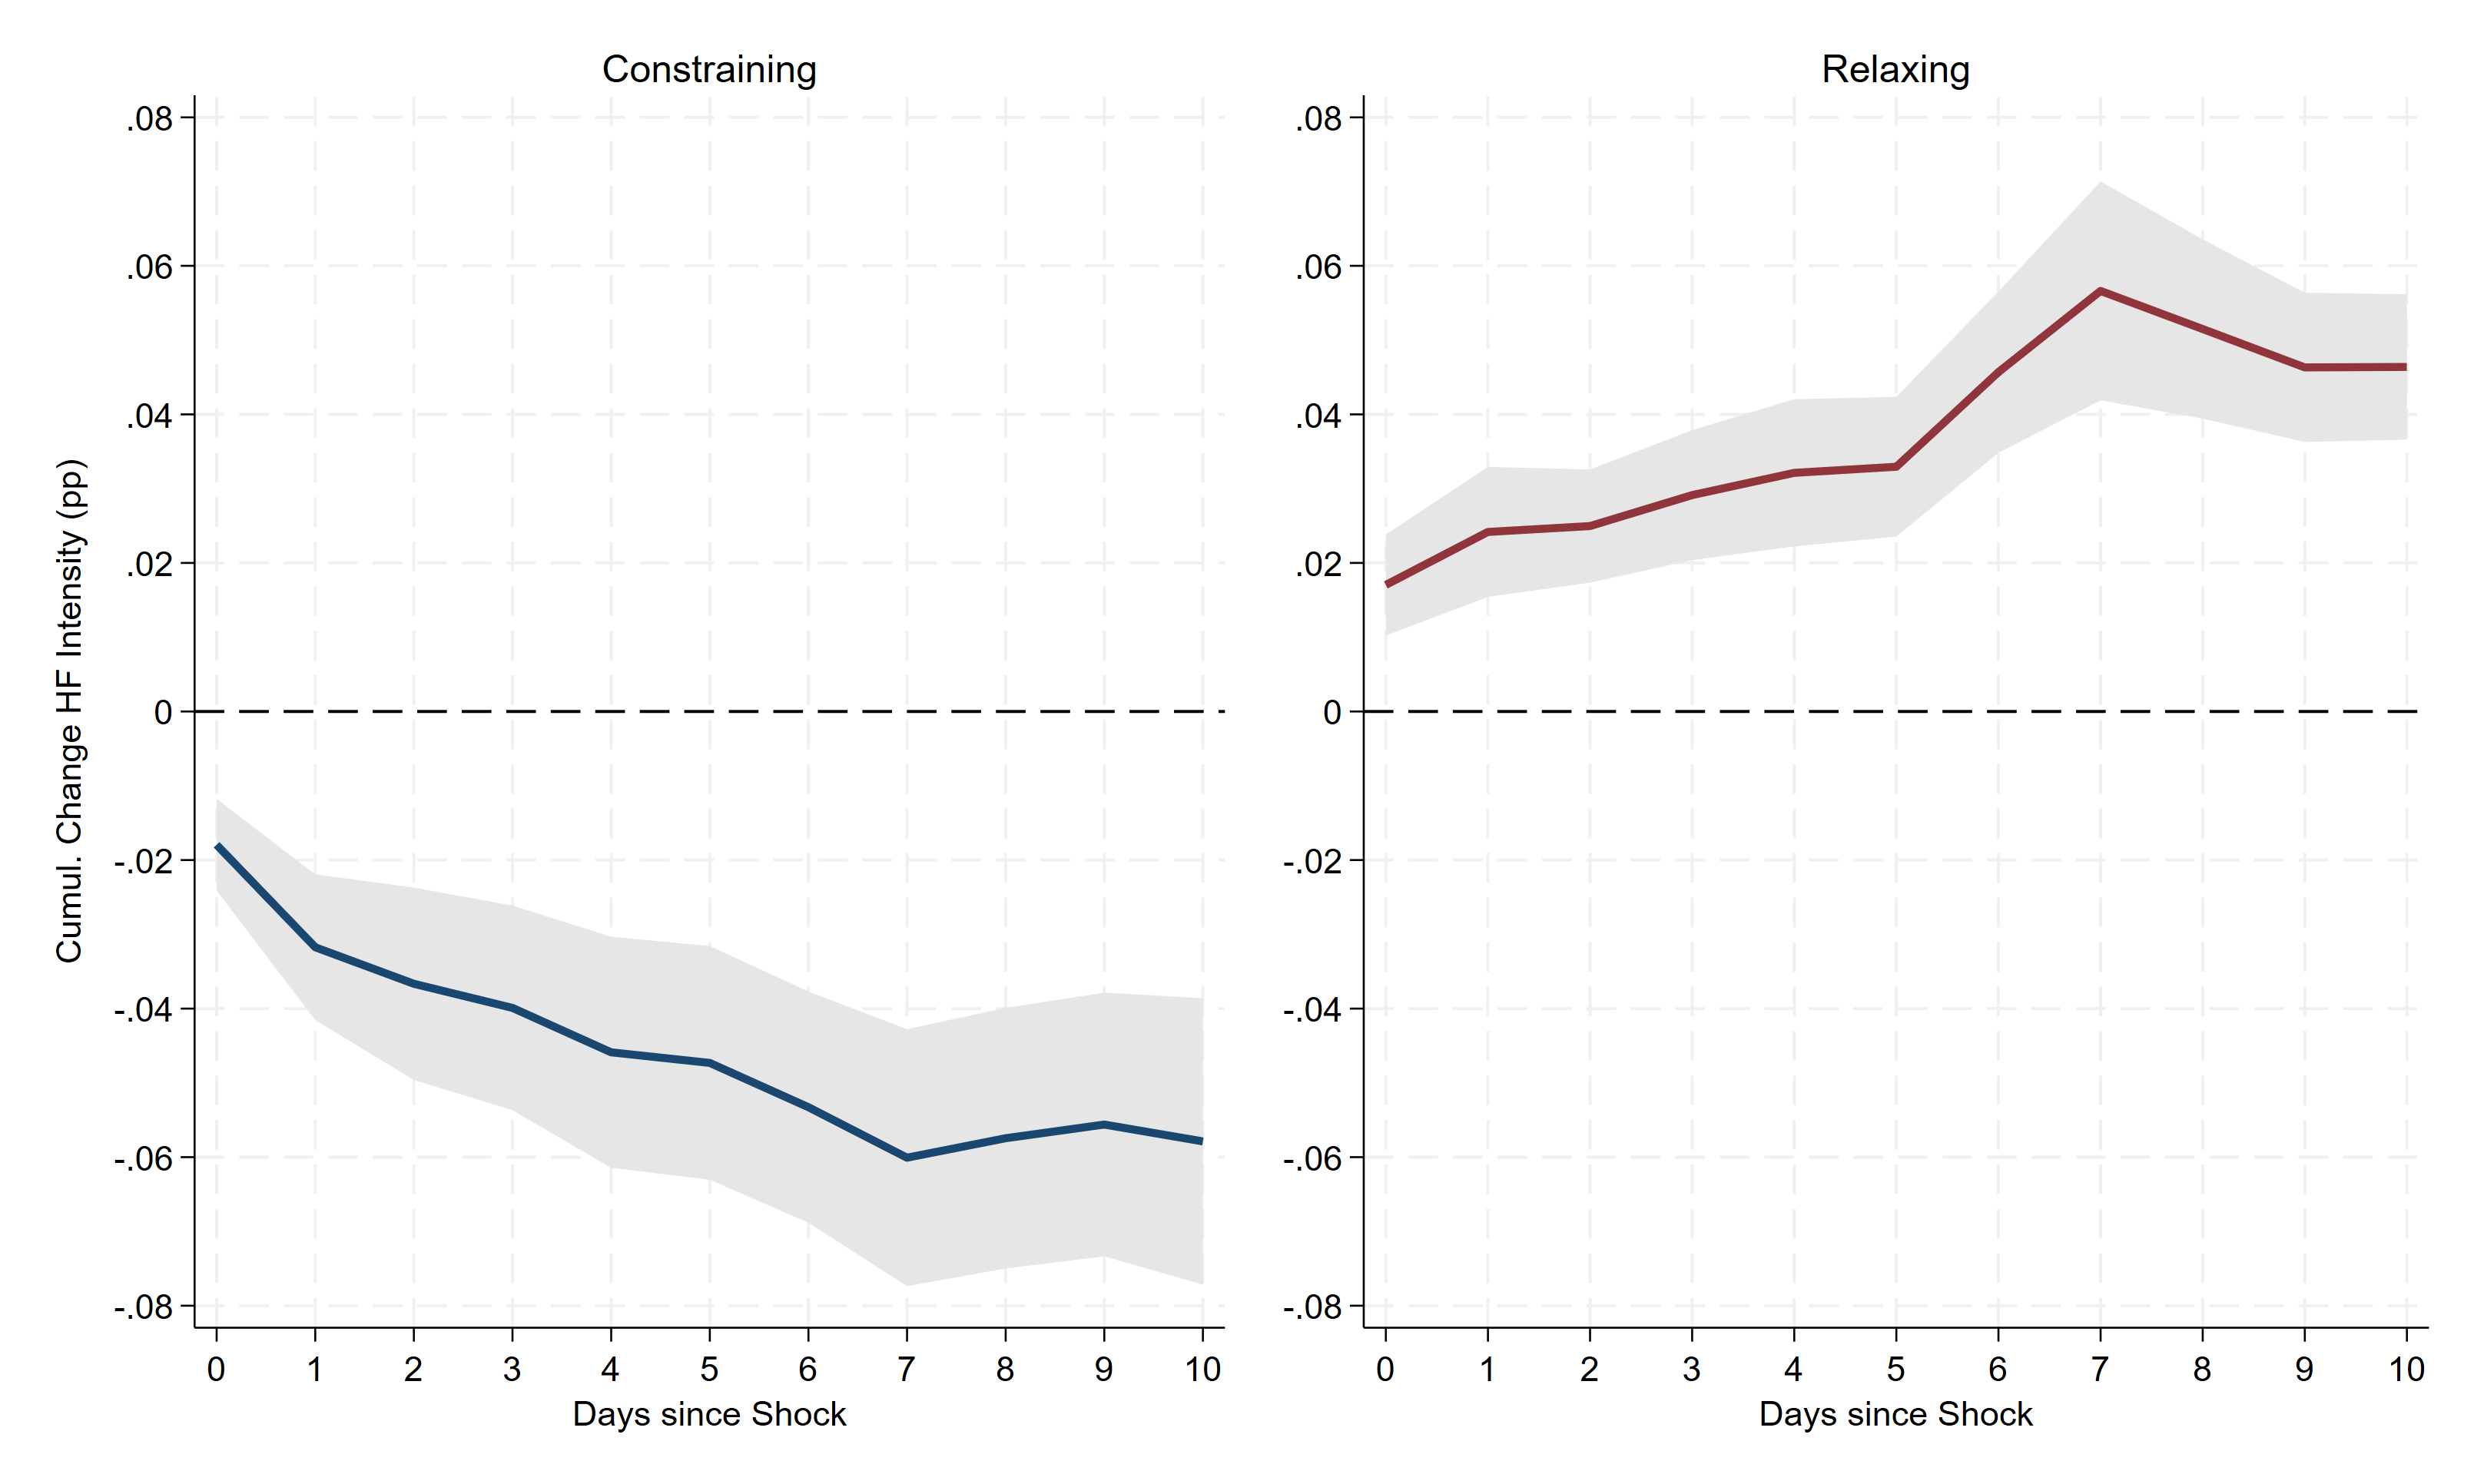
\includegraphics[width=\textwidth]{Figures/IR_on_momentum.png}
\vspace{-3mm}
% The note functions as the caption here
\caption*{\scriptsize \textit{Notes:} Dependent variable is the cumulative change in HF Intensity (pp) from $t-1$ to $t+h$. Intensity is measured as \% of amount issued. Sample restricted to overnight repo transactions. All specifications include bond fixed effects and duration $\times$ country $\times$ date fixed effects, with the latter absorbing the shock main effect. Identification of $\beta_h$ comes from within-cell variation in pre-shock positioning interacted with the shock. Standard errors clustered by date and bond. Shaded areas denote 90\% confidence intervals. \\ Sample period: 2021-01-01 -- 2025-11-01}
\label{fig:IR_overnight}
\end{figure}

To do so, I estimate the cumulative response of hedge fund intensity using local projections \citep{jorda2005}. This approach tests whether the position adjustments in the two regimes align with the predicted pattern. In the constraining regime, positions should contract as the shock erodes the collateral buffer. In the relaxing regime, positions should expand as the freed capacity is redeployed into the existing exposure.

Figure \ref{fig:IR_overnight} presents the impulse responses of hedge fund intensity to monetary policy shocks for overnight repo transactions. I focus on the overnight segment because these positions roll over daily and therefore allow for immediate adjustment, whereas term repo transactions are contractually locked until maturity and can adjust only with a lag. Appendix \ref{sec:term_repo_adjustment} reports the corresponding results for the term segment, which display the same qualitative patterns with a delay of approximately five days, in line with the maturity profile of those contracts.

The patterns are consistent with the predictions of Section \ref{sec:mechanism}. In the constraining regime, the cumulative change in hedge fund intensity is negative, consistent with funds reducing exposure as the shock erodes their collateral buffer. In the relaxing regime, the opposite pattern emerges. Rather than reducing exposure, hedge funds actively expand their positioning when the policy surprise moves prices in their favor. The near-symmetry between the contraction in the constraining regime and the expansion in the relaxing regime points towards constant-leverage targeting as the explanation \citep{adrian2014}, in which the same balance-sheet rule generates opposite position adjustments depending on the sign of the shock.

\section{Hedge Fund Directionality}
\label{sec:directionality}

The asymmetry result in Section \ref{subsec:asymmetries} establishes that the magnitude of the amplification does not depend on the sign of the position. Whether a fund is long or short, and whether the shock tightens or relaxes its constraint, the effect is comparable in size. A natural next question concerns the structure of the positions rather than their direction. Figure \ref{fig:HF_net} shows that the hedge fund sector moves between two configurations over the sample. In the periods around the hiking cycle it runs a book that is long Italian and short German government bonds. During the hiking cycle this structure collapses into a one-sided directional book. This section asks whether that distinction shapes the amplification. I answer it within the empirical strategy of Section \ref{sec:empirical_strategy}, interacting hedge fund positioning with the shock under the same fixed effects, and add only a measure of how directional each fund's book is.

The mechanism in Section \ref{sec:mechanism} describes the capital constraint at the level of an individual position. A fund, however, manages a single pool of capital against its entire bond book, so a shock erodes its capital in proportion to the net exposure of the whole portfolio rather than the exposure of any single bond. A fund that is long Italian and short German bonds of similar duration carries little net exposure to a parallel move in rates. A shock barely moves its capital and it has little reason to rebalance. A fund running a directional bond book absorbs the full capital loss and rebalances accordingly. The amplification that a given bond experiences should therefore depend on whether the funds holding it run a hedged or a directional bond book, and not only on how much they hold. A more hedged book corresponds to a higher effective margin in the mechanism of Section \ref{sec:mechanism}, so the directionality of a bond's holders is the cross-sectional counterpart to the single margin the numerical example assumes.

To take this to the data I construct a measure of book directionality at the bond level. For each fund and day I summarize its bond book by the directionality of its positions,

\begin{equation}
\text{Dir}_{f,t} = \frac{\left| \sum_{i} D_{i}\, q_{f,i,t} \right|}{\sum_{i} D_{i}\, \left| q_{f,i,t} \right|} ,
\end{equation}

\noindent where $q_{f,i,t}$ is the net position of fund $f$ in bond $i$ ahead of the shock, taken positive for long and negative for short, and $D_{i}$ is the duration of bond $i$. The numerator is the absolute net duration exposure of the book and the denominator is its gross duration exposure. The ratio equals zero when the long and short legs offset in duration terms and it approaches one when the book is one-sided. I then assign each bond the position weighted average of the directionality of the funds holding it,

\begin{equation}
\text{HolderDir}_{i,t} = \frac{\sum_{f} \left| q_{f,i,t} \right|\, \text{Dir}_{f,t}}{\sum_{f} \left| q_{f,i,t} \right|} .
\end{equation}

\noindent This variable lies between zero and one and is high when a bond is held mainly within directional books. As with the intensity measure, I average it over the five trading days before each shock so that it is predetermined.

Two points of interpretation matter. First, every fund in the data is a hedge fund, so the distinction is not between hedged and unhedged institutions but between bonds held within a hedged bond book and bonds held within a directional bond book, set against a baseline of bonds without hedge fund activity. Second, I observe only the cash leg of these positions. A book that looks directional in the cash market could in fact be hedged with derivatives that I do not observe, as in the cash-futures basis trade. This does not bias the comparison. If the hedge insulates the fund, the book carries little net exposure to the shock, so its presence in the directional group only pulls the measured difference toward zero and the estimate is conservative. If instead the bonds and the futures are financed and cleared with different counterparties, the two legs are margined separately, so the bond leg faces its own margin call and trades like the directional position the measure already treats it as.

\begin{figure}[t]
\centering
\caption{Aggregate hedge fund holder directionality over time}
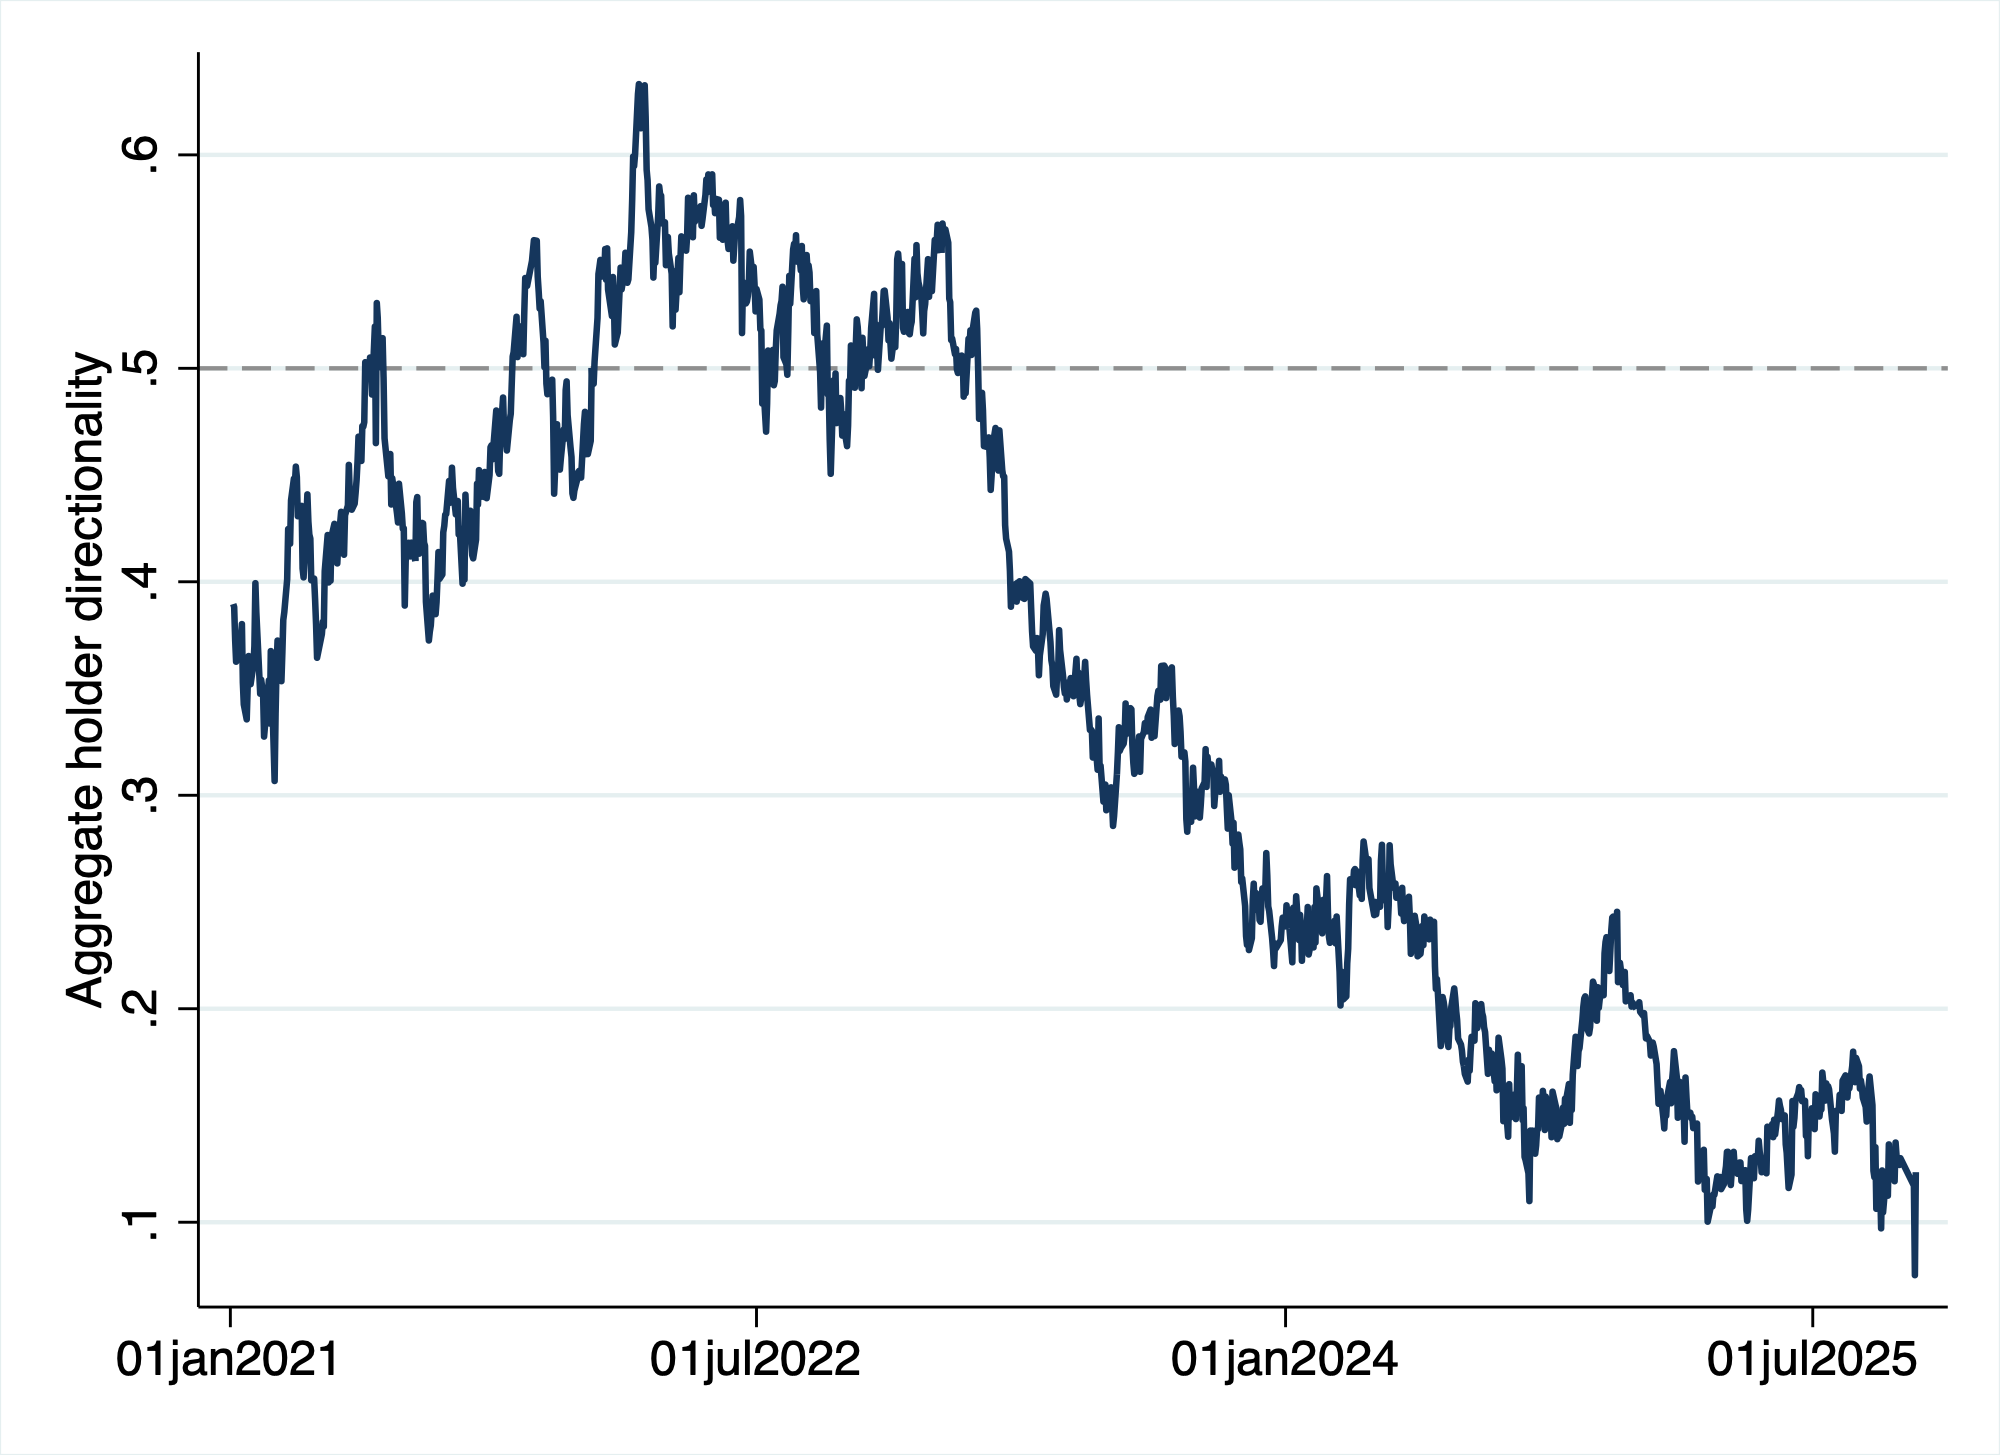
\includegraphics[width=\textwidth]{Figures/holder_dir_timeseries.png}
\caption*{\scriptsize \textit{Notes}: The figure plots the position weighted average across bonds of holder directionality on each date. Holder directionality is high when a bond is held mainly within directional books and low when it is held within hedged relative value books. The series shows pronounced low-frequency variation in how directional the sector is. Directionality is elevated through the first half of the sample and declines to its lowest levels in 2024 and 2025, when the relative value structure of Figure \ref{fig:HF_net} re-emerges. \\ Sample period: 2021-01-01 -- 2025-11-01}
\label{fig:holder_dir_ts}
\end{figure}

Figure \ref{fig:holder_dir_ts} plots the position weighted average of this measure across bonds over time. Directionality is elevated through the first half of the sample, which covers the run up to and the early part of the hiking cycle, and then declines steadily to its lowest levels in 2024 and 2025, when the sector returns to the relative value structure of Figure \ref{fig:HF_net}. The measure also varies in the cross section. Within the duration, country and date cells used throughout the paper, the average within-cell standard deviation of holder directionality is about 0.11, so bonds facing the same shock on the same day in the same duration and country segment still differ in the directionality of the books holding them. This within-cell variation is the source of identification for the results that follow.

I first add holder directionality to the intensity specification reported in Table \ref{tab:intensity}. Since holder directionality is defined only for bonds that hedge funds hold, I let it enter through the intensity term rather than as a separate regressor. I estimate

\begin{equation}
\begin{split}
\Delta y_{i,t} = {} & \beta_1 (\text{HF}_{i,t-1} \times \text{Shock}_{t}) + \beta_2 (\text{HF}_{i,t-1} \times \text{Shock}_{t} \times \text{HolderDir}_{i,t-1}) \\
& + \beta_3 (\text{HF}_{i,t-1} \times \text{HolderDir}_{i,t-1}) + \gamma \mathbf{X}_{i,t-1} + \theta_{k} + \varepsilon_{i,t}
\end{split}
\end{equation}

\noindent where $\text{HF}_{i,t-1}$ is Log HF Intensity and $\text{Shock}_{t}$ is the monetary policy shock. The coefficient of interest is $\beta_2$, which measures how the amplification per unit of positioning changes as the holders of a bond become more directional. Column (1) of Table \ref{tab:directionality} reports $\beta_2 = 0.236$, significant at the five percent level. The amplification per unit of hedge fund intensity is larger for bonds held within directional books, holding the amount of positioning fixed.

Columns (2) and (3) report a less parametric version of the same result. In Column (2) I split the hedge fund bonds at the median of holder directionality and interact each group with the shock against the baseline of bonds without hedge fund activity. The amplification of bonds held within hedged books is 0.098, while that of bonds held within directional books is 0.363. A Wald test rejects equality of the two coefficients with an F statistic of 24.8. Column (3) replaces the binary split with quartiles. The interaction rises monotonically from 0.057 in the most hedged quartile, which is not statistically distinguishable from zero, to 0.367 in the most directional quartile, and a test rejects equality of the extreme quartiles with an F statistic of 28.3. The amplification is concentrated among the bonds held within the most directional books and is essentially absent when the book is hedged.

\begin{table}[t]
\centering
\caption{\textbf{Hedge Fund Directionality and Yield Amplification}}
\footnotesize
\setlength{\tabcolsep}{10pt}
\renewcommand{\arraystretch}{1.1}
\begin{tabular}{l c c c}
\toprule
\textbf{Dependent Variable:} & \multicolumn{3}{c}{\textbf{$\Delta$ Bond Yield (bps)}} \\
\cmidrule(lr){2-4}
 & \textbf{(1) Continuous} & \textbf{(2) Categorical} & \textbf{(3) Quartile} \\
\midrule
\textit{Continuous interaction} & & & \\
\textbf{Log HF Intensity $\times$ Shock $\times$ Holder Dir.} & \textbf{0.236**} & & \\
 & (0.100) & & \\
Log HF Intensity $\times$ Shock & 0.066 & & \\
 & (0.048) & & \\
\addlinespace
\textit{By holder regime (relative to no HF)} & & & \\
Hedged book $\times$ Shock & & 0.098*** & \\
 & & (0.034) & \\
\textbf{Directional book $\times$ Shock} & & \textbf{0.363***} & \\
 & & (0.057) & \\
\addlinespace
\textit{By holder directionality quartile (relative to no HF)} & & & \\
Q1 most hedged $\times$ Shock & & & 0.057 \\
 & & & (0.035) \\
Q2 $\times$ Shock & & & 0.137*** \\
 & & & (0.037) \\
Q3 $\times$ Shock & & & 0.361*** \\
 & & & (0.065) \\
\textbf{Q4 most directional $\times$ Shock} & & & \textbf{0.367***} \\
 & & & (0.057) \\
\midrule
Controls & Yes & Yes & Yes \\
Bond FE & Yes & Yes & Yes \\
Duration $\times$ Date $\times$ Country FE & Yes & Yes & Yes \\
\midrule
Observations & 472,320 & 472,320 & 472,320 \\
\bottomrule
\end{tabular}
\label{tab:directionality}

\vspace{1ex}
\raggedright\scriptsize
\textit{Notes:} The table reports the amplification of bond yields to monetary policy shocks as a function of the directionality of the hedge funds holding each bond. The dependent variable is the daily yield change in basis points. Holder directionality is the position weighted average across a bond's hedge fund holders of each fund's absolute net duration exposure over its gross duration exposure, measured over the five trading days before the shock and scaled to lie between zero and one. Column (1) interacts Log HF Intensity and the shock with holder directionality, with holder directionality entering only through the intensity term. Columns (2) and (3) compare bonds held by hedge funds, split at the median and into quartiles of holder directionality, against the baseline of bonds without hedge fund activity. Log HF Intensity is the natural log of one plus the average absolute net position over the prior five trading days scaled by amount outstanding. Shock is the change in the two year OIS rate during the ECB event window. All columns include the bid-ask spread and a CTD indicator as controls, bond fixed effects, and duration by country by date fixed effects, with the latter absorbing the shock main effect. A Wald test rejects equality of the hedged and directional coefficients in Column (2) with $F=24.8$ and equality of the extreme quartiles in Column (3) with $F=28.3$. Standard errors clustered by business date and bond in parentheses. *** p$<$0.01, ** p$<$0.05, * p$<$0.10. \\ Sample period: 2021-01-01 -- 2025-11-01
\end{table}

Because the directional configuration coincides with the hiking cycle, one might worry that the result reflects the monetary environment rather than the positioning. The within-cell identification addresses this concern directly. The fixed effects compare bonds facing the same shock on the same day in the same maturity and country segment, so the common monetary environment is absorbed and the estimate comes from cross-sectional differences in which funds hold each bond.

\begin{figure}[t]
    \centering
    \caption{Persistence of the amplification by holder directionality}
    \begin{subfigure}[t]{0.49\textwidth}
        \centering
        \caption{Bonds in hedged books}
        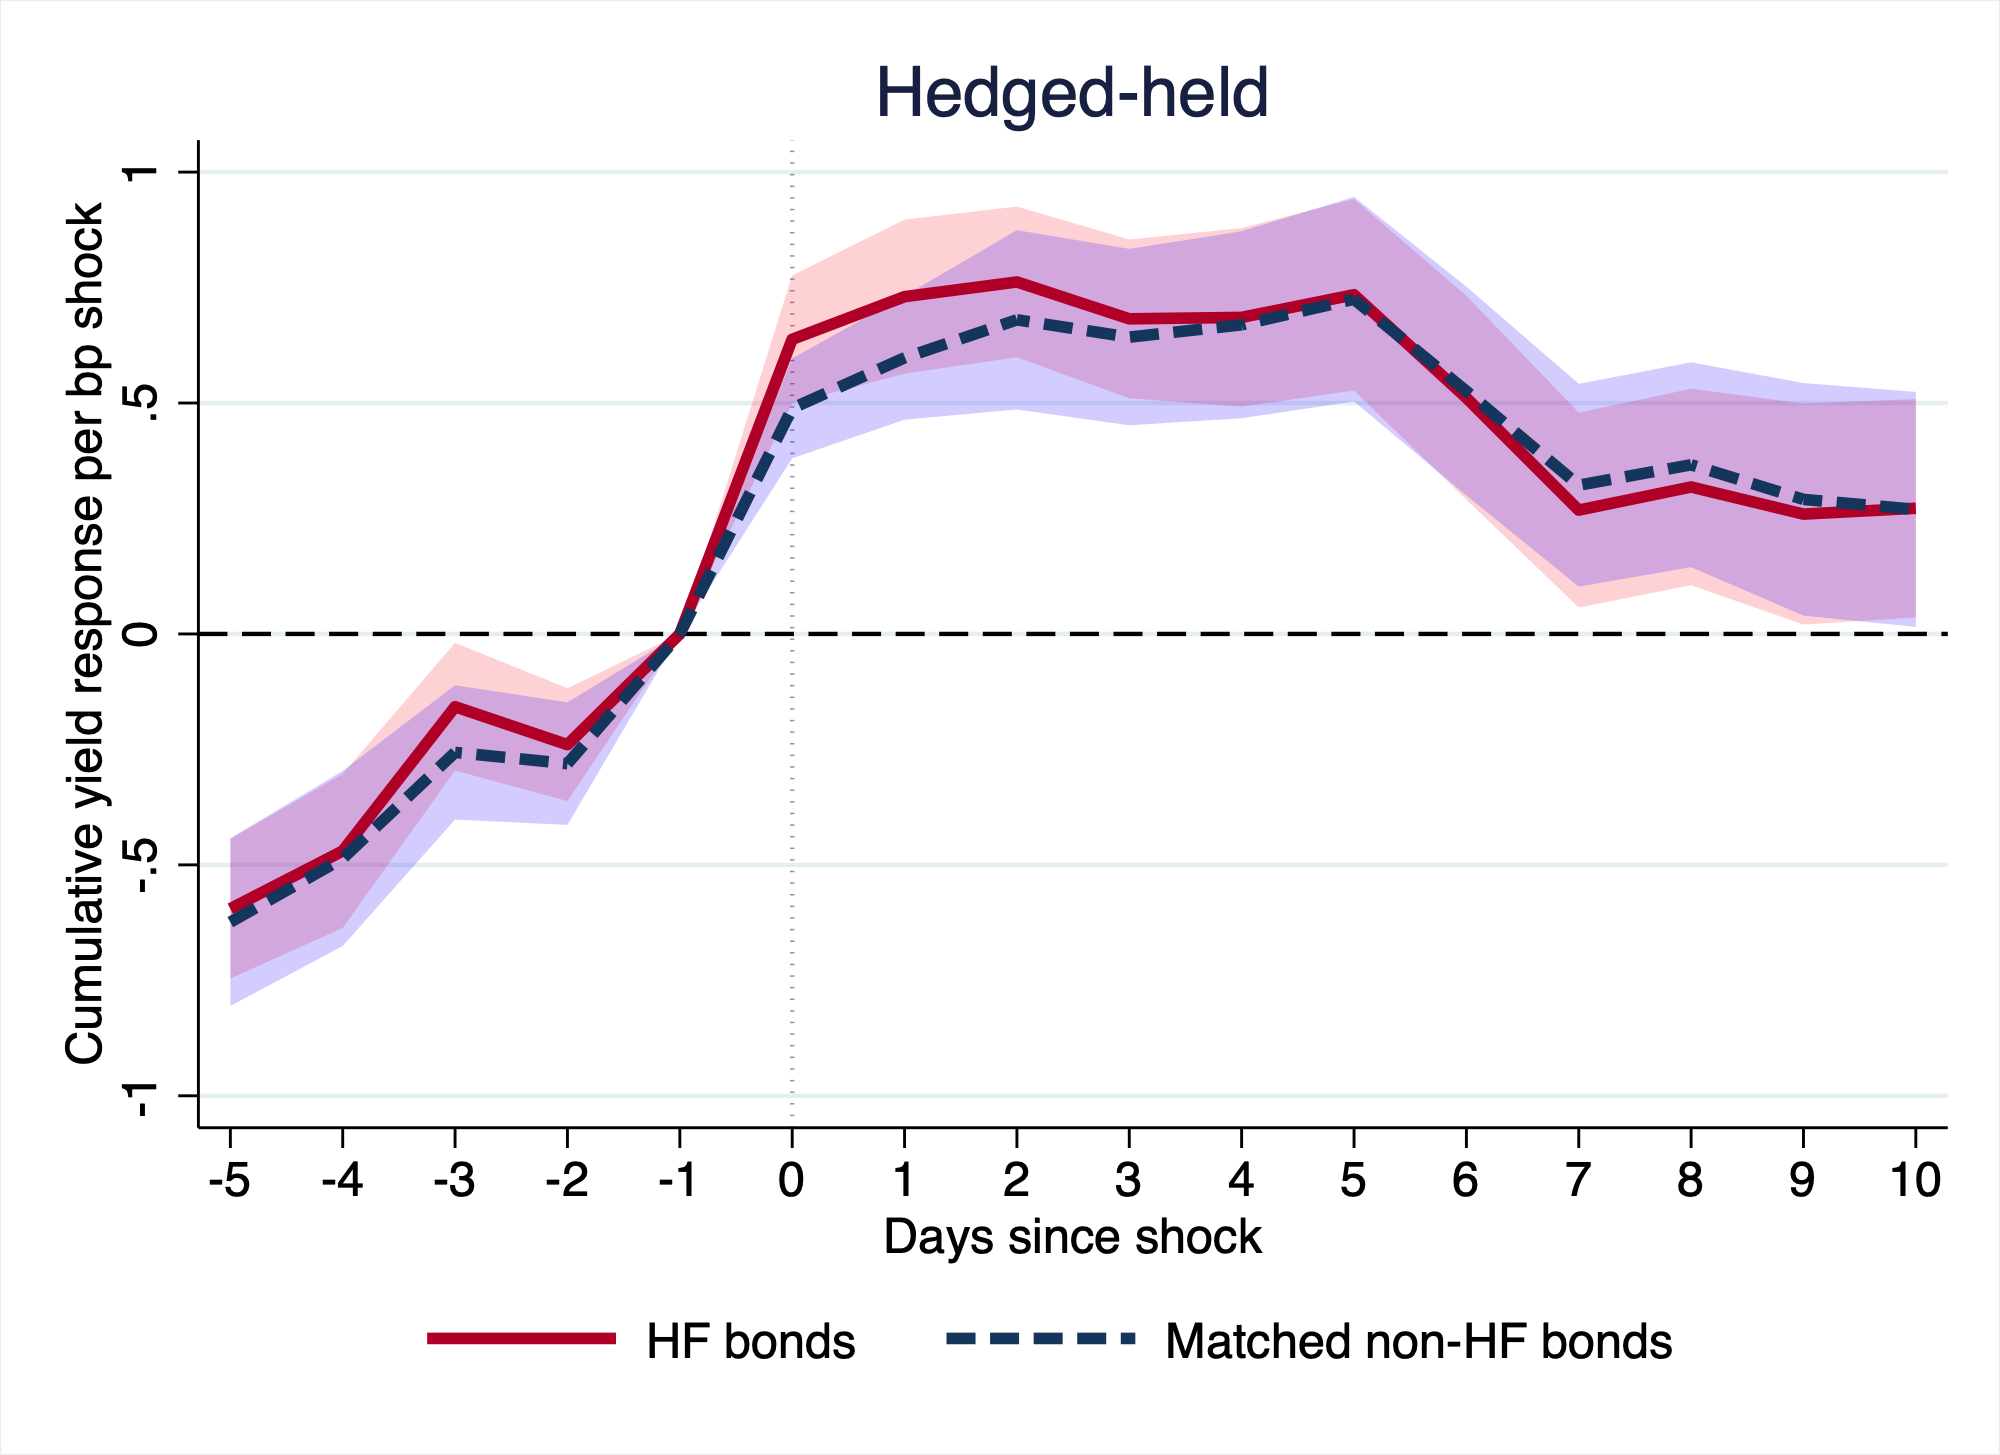
\includegraphics[width=\textwidth]{Figures/IR_holder_dir_hedged.png}
        \label{fig:IR_holder_hedged}
    \end{subfigure}
    \hfill
    \begin{subfigure}[t]{0.49\textwidth}
        \centering
        \caption{Bonds in directional books}
        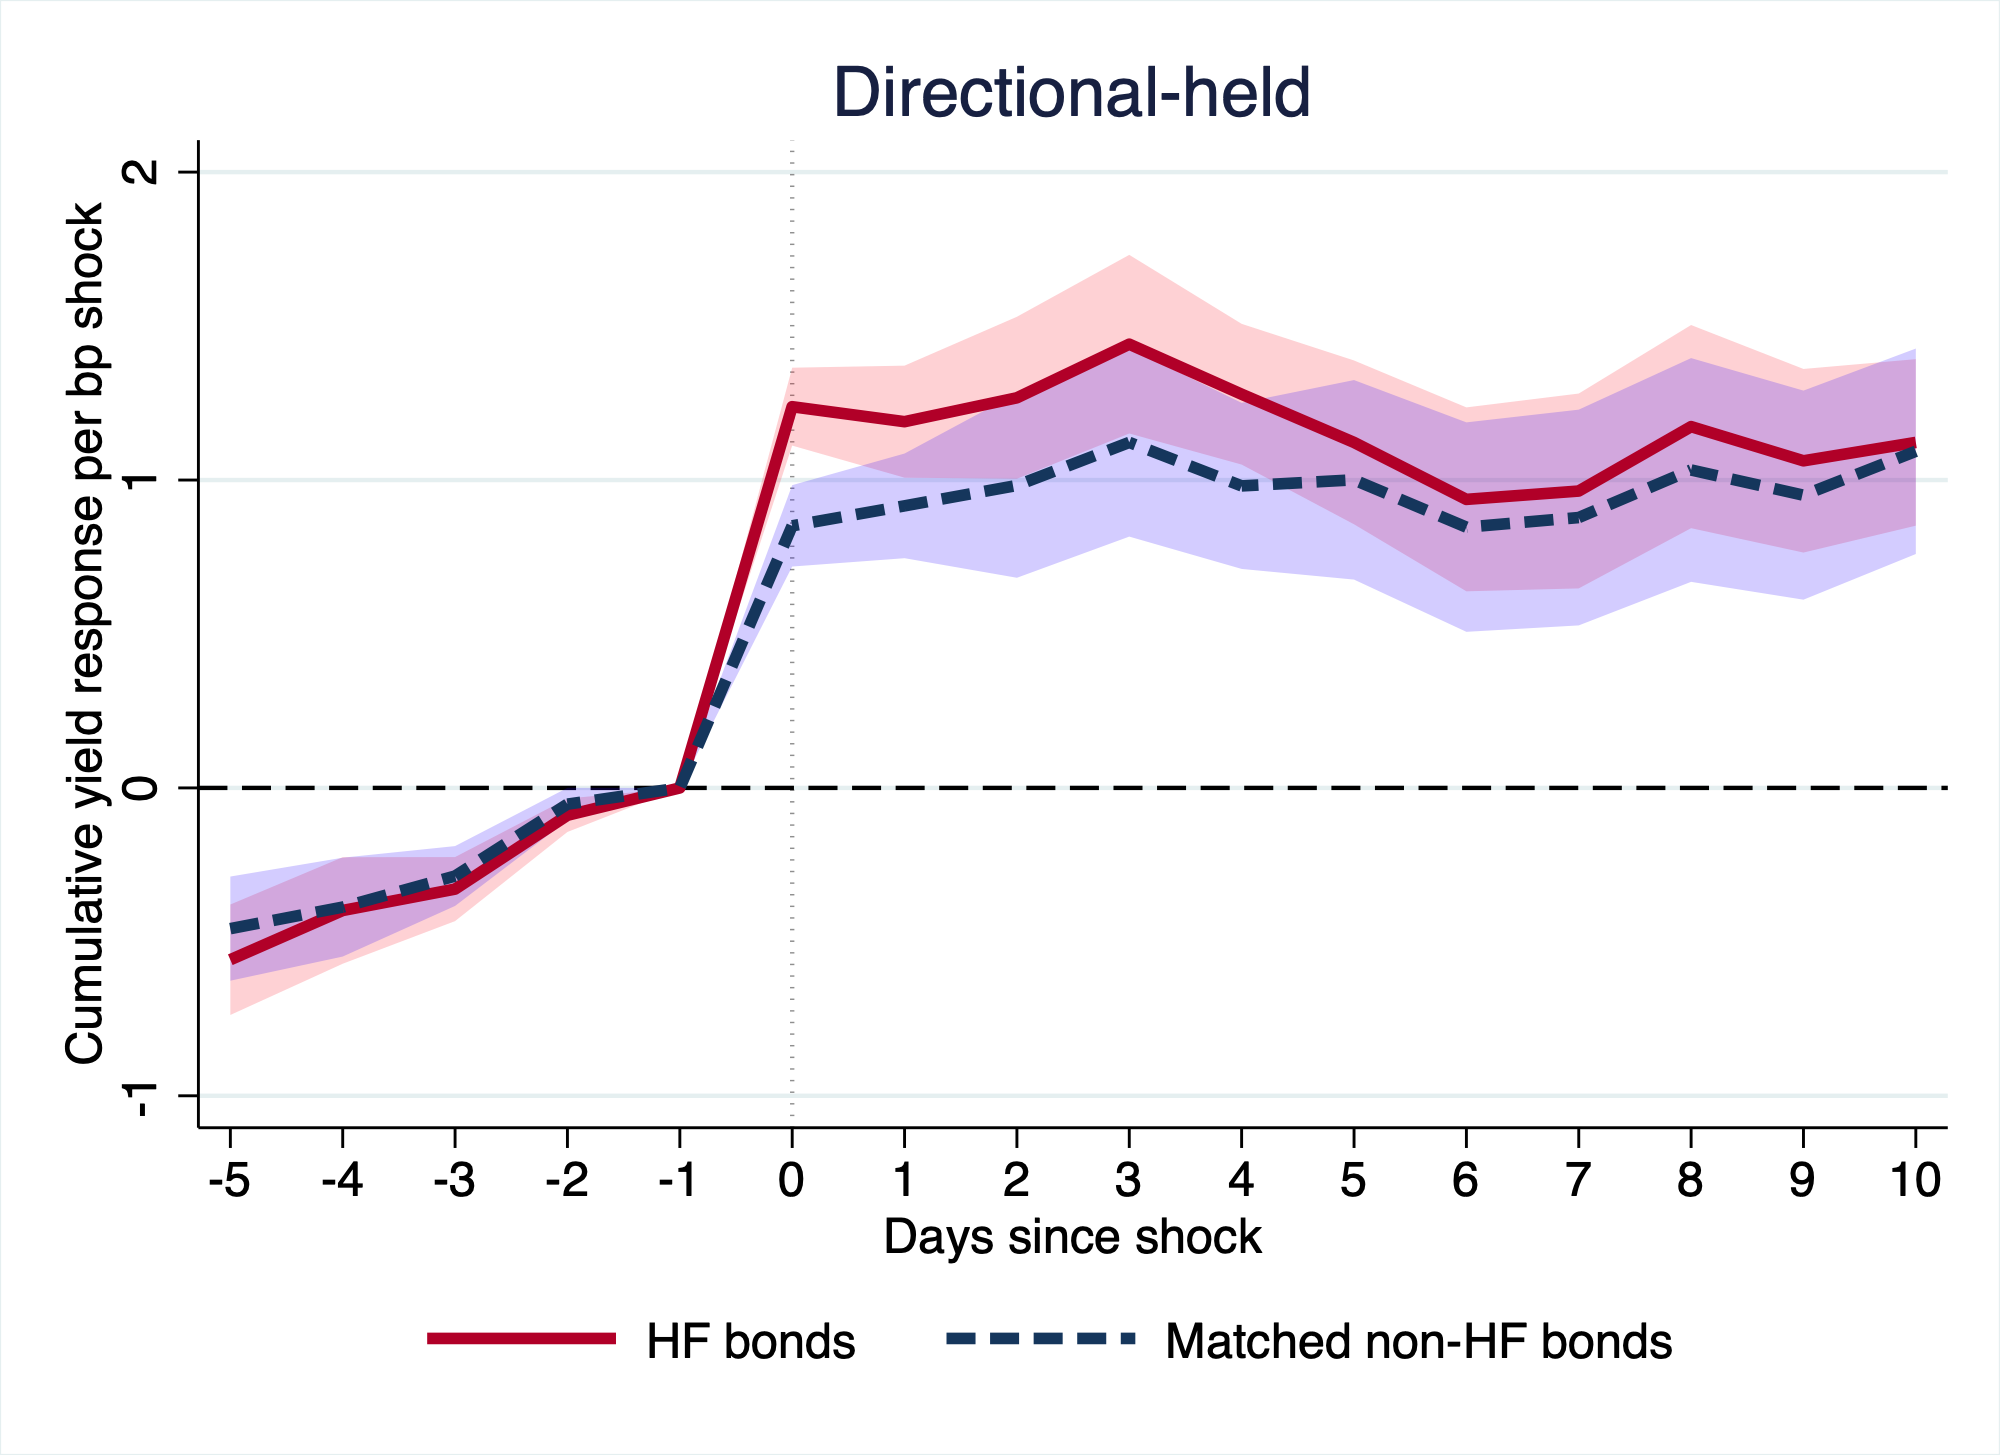
\includegraphics[width=\textwidth]{Figures/IR_holder_dir_directional.png}
        \label{fig:IR_holder_directional}
    \end{subfigure}
    \caption*{\scriptsize \textit{Notes:} The figure plots cumulative yield responses per basis point of monetary policy shock over a window from $h=-5$ to $h=10$ trading days, estimated by local projections \citep{jorda2005} on the matched sample of Section \ref{subsec:baseline}. Each hedge fund bond is matched to an observationally similar bond without hedge fund activity. Panel (a) restricts the hedge fund bonds to those in hedged books and Panel (b) to those in directional books, where the split is at the median of holder directionality. The solid line is the response of hedge fund bonds and the dashed line the response of their matched counterparts. Shaded areas denote 90\% confidence intervals clustered by the matching cell. \\ Sample period: 2021-01-01 -- 2025-11-01}
    \label{fig:IR_holder_dir}
\end{figure}

To trace the dynamics of the amplification I estimate impulse responses using the local projections of \citet{jorda2005}, following the matched sample design of Section \ref{subsec:baseline}. I match each hedge fund bond to an observationally similar bond without hedge fund activity and plot the cumulative yield response per basis point of shock for both legs, separately for bonds in hedged books and bonds in directional books. Figure \ref{fig:IR_holder_dir} reports the result.

The two panels differ in exactly the way the mechanism predicts. In Panel (b) the bonds in directional books overshoot their matched counterparts on impact and then revert toward a common level over the following days, the same overshooting pattern documented for the full sample in Section \ref{subsec:baseline}. In Panel (a) the bonds in hedged books barely depart from their matched counterparts at any horizon. The amplification that drives the baseline result therefore operates through the bonds in directional books and switches off when the book is hedged.

These results carry two implications. First, they sharpen the evidence for overshooting. The amplification appears only for bonds held within directional books, which is exactly where the leverage mechanism predicts a dislocation, and it reverts toward the matched level over the following days rather than persisting. This concentration is hard to reconcile with a price-discovery account, in which hedge fund trading would push yields toward fundamentals and the response would not unwind. Second, the result speaks to how the sector should be monitored. The destabilizing potential of leveraged positioning is not captured by its size alone. The same amount of positioning amplifies a shock when it sits within a directional book and is close to neutral when it sits within a hedged book. Supervisors gauging the systemic footprint of hedge funds therefore need to account for the directionality of the book, and not only the gross size of the positions.


\section{Robustness}
\label{sec:robustness_main}
\subsection{Volatility-Standardized Yield Changes}
\label{subsec:GARCH}

The duration-by-country-by-date fixed effects used in Section \ref{sec:empirical_results} ensure that bonds with similar rate sensitivity facing the same shock are compared against each other, and Table \ref{tab:volatility} shows that within these cells the average absolute yield change of hedge fund bonds is statistically indistinguishable from that of their peers on regular days. This addresses the concern that hedge funds systematically select bonds with higher unconditional volatility. A more subtle concern is that bond yield volatility is time-varying and might cluster in high-volatility regimes. Figure \ref{fig:exceedance_probability} documents that shock days fall disproportionately into such regimes. Two bonds with identical unconditional volatility can therefore differ in their conditional volatility on any given day. If hedge fund bonds happen to be in elevated conditional volatility states on announcement days specifically, the interaction coefficient in the baseline specification could partly reflect this state-dependent volatility rather than the amplification of leveraged positioning. To address this concern, I normalize each bond's daily yield change by its own conditional volatility estimated from a GARCH(1,1) model, which rescales the dependent variable into units of the bond's own typical daily variation at that point in time.

For each bond in the sample, I estimate a GARCH(1,1) model on the time series of daily yield changes, restricting the estimation sample to non-announcement days. The model takes the form
\begin{align*}
\Delta y_{i,t} &= \mu_i + \varepsilon_{i,t}, \qquad \varepsilon_{i,t} \sim \mathcal{N}(0, \sigma^2_{i,t}), \\
\sigma^2_{i,t} &= \omega_i + \alpha_i \varepsilon^2_{i,t-1} + \beta_i \sigma^2_{i,t-1}.
\end{align*}
where $\Delta y_{i,t}$ is the daily yield change of bond $i$ on day $t$, $\mu_i$ is the bond-specific mean, $\varepsilon_{i,t}$ is the innovation with conditional variance $\sigma^2_{i,t}$, $\omega_i$ is the long-run variance parameter, $\alpha_i$ governs the response of conditional variance to past innovations, and $\beta_i$ captures the persistence of volatility.

Restricting the estimation to non-announcement days ensures that the estimated parameters describe each bond's baseline volatility dynamics rather than absorbing the announcement-day reactions that the analysis is designed to study. Bonds with fewer than 250 non-announcement observations are excluded to ensure stable parameter estimates, which reduces the panel to approximately 370,000 bond-day observations. Using the fitted parameters, I then construct a one-step-ahead conditional variance forecast $\hat{\sigma}^2_{i,t}$ for every bond-day in the sample, and standardize the yield change as $\Delta \tilde{y}_{i,t} = \Delta y_{i,t} / \hat{\sigma}_{i,t}$. The standardized variable measures each yield change in units of the bond's own conditional standard deviation on that day, so two bonds in different volatility regimes contribute comparably to the estimation. I re-estimate the specifications in Section \ref{sec:empirical_results} based on this standardized dependent variable.


\begin{table}[t]
\centering
\caption{\textbf{Hedge Fund Amplification on GARCH-Standardized Yield Changes}}
\footnotesize
\setlength{\tabcolsep}{9pt}
\renewcommand{\arraystretch}{1.1}
\begin{tabular}{l c c c c}
\toprule
\textbf{Dependent Variable:} & \multicolumn{4}{c}{\textbf{Standardized $\Delta$ Bond Yield ($\sigma$ units)}} \\
\cmidrule(lr){2-5}
 & (1) & (2) & (3) & (4) \\
 & & & Constraining & Relaxing \\
\midrule
\textit{Main Interaction} & & & & \\
\textbf{HF Involved $\times$ Shock} & \textbf{0.043***} & & & \\
 & (0.010) & & & \\
\textbf{Log HF Intensity $\times$ Shock} & & \textbf{0.020***} & \textbf{0.016***} & \textbf{0.031***} \\
 & & (0.004) & (0.004) & (0.008) \\
\addlinespace
\textit{Direct Effects} & & & & \\
HF Involved & $-$0.007 & & & \\
 & (0.010) & & & \\
Log HF Intensity & & $-$0.004 & $-$0.005 & $-$0.004 \\
 & & (0.003) & (0.003) & (0.004) \\
\addlinespace
\textit{Controls} & & & & \\
Bid-Ask Spread & $-$0.056*** & $-$0.057*** & $-$0.056*** & $-$0.055*** \\
 & (0.015) & (0.015) & (0.015) & (0.015) \\
CTD Flag & $-$0.001 & $-$0.000 & $-$0.000 & $-$0.000 \\
 & (0.005) & (0.005) & (0.005) & (0.005) \\
\midrule
Bond FE & Yes & Yes & Yes & Yes \\
Duration $\times$ Date $\times$ Country FE & Yes & Yes & Yes & Yes \\
\midrule
Observations & 374,058 & 374,058 & 370,520 & 370,449 \\
R-squared & 0.681 & 0.681 & 0.675 & 0.677 \\
\bottomrule
\end{tabular}
\label{tab:garch_robustness}

\vspace{1ex}
\raggedright\scriptsize
\textit{Notes:} This table re-estimates the main specifications with the dependent variable replaced by the GARCH-standardized daily yield change. For each bond, conditional volatility $\hat{\sigma}_{i,t}$ is estimated from a GARCH(1,1) model fit on non-shock days, and $\Delta y_{i,t}$ is normalized by $\hat{\sigma}_{i,t}$. The standardized dependent variable is therefore expressed in units of each bond's own conditional standard deviation, removing differences in time-varying volatility across bonds. \textit{HF Involved} is a dummy indicating presence of offshore hedge fund repo activity. \textit{Log HF Intensity} is the natural log of one plus the average absolute hedge fund net position over the prior five trading days, scaled by the bond's total amount outstanding. \textit{Shock} is the 2-year OIS rate change during the ECB monetary event window. Column (1) corresponds to Column (4) in Table~\ref{tab:baseline}, Column (2) to Column (4) in Table~\ref{tab:intensity}, and Columns (3) and (4) to Columns (1) and (2) in Table~\ref{tab:asymmetry}. The Shock main effect is absorbed by the fixed effects. Standard errors are clustered by business date and bond. *** p$<$0.01, ** p$<$0.05, * p$<$0.10. \\ Sample period: 2021-01-01 -- 2025-11-01
\end{table}

Table~\ref{tab:garch_robustness} presents the estimation results on the standardized dependent variable. Across all four specifications, the interaction coefficient remains positive and statistically significant at the 1\% level. Column (1) re-estimates the binary specification of Column (4) in Table~\ref{tab:baseline} and yields an interaction coefficient of 0.043. Column (2) replicates the continuous intensity specification of Column (4) in Table~\ref{tab:intensity} and yields a coefficient of 0.020. Columns (3) and (4) split the continuous specification into the constraining and relaxing regimes, mirroring Table~\ref{tab:asymmetry}. The interaction coefficient is 0.016 in the constraining regime and 0.031 in the relaxing regime, both significant at the 1\% level. The direct effects of HF Involved and Log HF Intensity are statistically indistinguishable from zero across all specifications, indicating that bonds with hedge fund positioning do not exhibit abnormally large standardized yield changes on regular days.

The coefficients in Table~\ref{tab:garch_robustness} are measured in standard deviation units rather than basis points, but they can be mapped back to the baseline magnitudes through the average conditional volatility in the sample. The average $\hat{\sigma}_{i,t}$ across bond-days is approximately 6 basis points, so the binary interaction coefficient of 0.043 in Column (1) implies an additional yield reaction of roughly $0.043 \times 6 \approx 0.26$ basis points per basis point of shock, close to the baseline estimate of 0.291 in Column (4) of Table~\ref{tab:baseline}. The continuous intensity coefficient of 0.020 in Column (2) implies an additional reaction of roughly $0.020 \times 6 \approx 0.12$ basis points per basis point of shock, comparable to the baseline estimate of 0.164 in Column (4) of Table~\ref{tab:intensity}. The corresponding coefficients in the constraining and relaxing regimes map to $0.016 \times 6 \approx 0.10$ and $0.031 \times 6 \approx 0.19$ basis points per basis point of shock, comparable to the baseline estimates of 0.140 and 0.224 in Table~\ref{tab:asymmetry}. The amplification of hedge fund positioning therefore survives normalization by each bond's own time-varying conditional volatility, indicating that the effect documented in the main analysis does not reflect hedge fund bonds being in elevated volatility regimes on announcement days, but rather the additional yield reactivity that arises from leveraged positioning interacting with the shock.

\subsection{CDS-based shocks}
\label{subsec:cds_shocks}

The monetary policy surprises used so far provide a clean laboratory because they are exogenous and sharply timed, but the amplification mechanism is not specific to monetary news. The framework in Section \ref{sec:mechanism} predicts that leveraged positioning amplifies yields whenever an unusually large price change interacts with pre-existing positions, regardless of what moves the price. A natural way to test the external validity of the mechanism is therefore to subject it to an independent shock that originates from a different economic source. To this end, I construct shocks from large changes in Italian sovereign credit default swap spreads. Because these shocks reflect credit risk rather than the risk-free rate, they are economically distinct from the monetary surprises and provide a test of whether the same leveraged positioning channel operates when the trigger is sovereign credit risk rather than monetary policy. I focus on Italy only for two reasons. First, German sovereign CDS is thinly traded and exhibits little price variation over the sample, so a comparable shock measure cannot be constructed for it. Second, German bunds are sometimes considered a euro area safe haven \citep[e.g.,][]{ehrmann2017}, so a credit shock that widens spreads elsewhere might coincide with a flight-to-safety in German yields. The sign of the yield response to a credit shock would therefore differ across the two issuers, which would confound the constraining and relaxing regime classification that the mechanism relies on. Restricting the credit shock analysis to Italy avoids this and keeps the sign mapping between the shock and the yield response unambiguous.

I measure sovereign credit risk using the five year Italian sovereign CDS spread denominated in US dollars. The dollar-denominated contract isolates credit risk more cleanly than its euro-denominated counterpart, which is contaminated by the correlation between Italian default risk and a depreciation of the euro. To separate the unanticipated component of the credit shock from movements that are predictable or potentially related to the trading I study, I residualize the daily change in the CDS spread on its own lag, the lagged change in the V2X equity volatility index, and the lagged aggregate net position of the hedge fund sector in Italian sovereign bonds. The residual from this regression is used to construct the credit shock. I define a credit shock day as a day on which the absolute shock falls in the 2\% most extreme part of its distribution.\footnote{Figure \ref{fig:exceedance_probability_cds} shows that credit shock days carry substantially more tail risk in bond yields than ordinary days, mirroring the pattern for monetary surprises.}\textsuperscript{,}\footnote{Results are robust to alternative thresholds.} Finally, because a credit shock that coincides with a monetary policy announcement could not be attributed to credit risk alone, I exclude any credit shock day that falls on or adjacent to an ECB monetary event, so that the credit shock is identified entirely off non-monetary variation.

Table \ref{tab:cds_robustness} reports the estimates. Column (1) uses the binary indicator of hedge fund presence and Columns (2) to (4) use the continuous intensity measure. Columns (3) and (4) split the sample into the constraining and the relaxing regime in the same way as in the baseline analysis. Across all four specifications the interaction between hedge fund positioning and the credit shock is positive and statistically significant at the 1\% level. In the binary specification the coefficient on the interaction is 0.225, and in the continuous specification it is 0.107. The split by regime yields an interaction coefficient of 0.129 in the constraining regime and 0.117 in the relaxing regime. The direct effects of hedge fund presence and hedge fund intensity are small and statistically insignificant throughout, indicating that bonds with hedge fund positioning do not display different yield changes on days without a credit shock.

\begin{table}[t]
\centering
\caption{\textbf{Hedge Fund Amplification under Credit Shocks}}
\footnotesize
\setlength{\tabcolsep}{9pt}
\renewcommand{\arraystretch}{1.1}
\begin{tabular}{l c c c c}
\toprule
\textbf{Dependent Variable:} & \multicolumn{4}{c}{\textbf{$\Delta$ Bond Yield (bps)}} \\
\cmidrule(lr){2-5}
 & (1) & (2) & (3) & (4) \\
 & & & Constraining & Relaxing \\
\midrule
\textit{Main Interaction} & & & & \\
\textbf{HF Involved $\times$ Shock} & \textbf{0.225***} & & & \\
 & (0.058) & & & \\
\textbf{Log HF Intensity $\times$ Shock} & & \textbf{0.107***} & \textbf{0.129***} & \textbf{0.117***} \\
 & & (0.034) & (0.040) & (0.042) \\
\addlinespace
\textit{Direct Effects} & & & & \\
HF Involved & $-$0.030 & & & \\
 & (0.045) & & & \\
Log HF Intensity & & $-$0.021 & $-$0.022 & $-$0.020 \\
 & & (0.022) & (0.022) & (0.021) \\
\addlinespace
\textit{Controls} & & & & \\
Bid-Ask Spread & $-$0.427*** & $-$0.417*** & $-$0.413*** & $-$0.409*** \\
 & (0.113) & (0.113) & (0.114) & (0.113) \\
CTD Flag & 0.041 & 0.046 & 0.037 & 0.048 \\
 & (0.046) & (0.046) & (0.046) & (0.049) \\
\midrule
Bond FE & Yes & Yes & Yes & Yes \\
Duration $\times$ Date $\times$ Country FE & Yes & Yes & Yes & Yes \\
\midrule
Observations & 297,411 & 297,411 & 295,028 & 294,834 \\
R-squared & 0.721 & 0.721 & 0.719 & 0.719 \\
\bottomrule
\end{tabular}
\label{tab:cds_robustness}

\vspace{1ex}
\raggedright\scriptsize
\textit{Notes:} This table re-estimates the main specifications using the sovereign credit shock in place of the monetary policy surprise. The credit shock is the residual from a regression of the daily change in the five-year US dollar Italian sovereign CDS spread on its own lag, the lagged change in the V2X index, and the lagged aggregate net hedge fund position in Italian sovereign bonds. A credit shock day is a day on which the absolute residual falls in the 2\% most extreme part of its distribution, and days on or adjacent to an ECB monetary event are excluded. \textit{HF Involved} is a dummy indicating presence of offshore hedge fund repo activity. \textit{Log HF Intensity} is the natural log of one plus the average absolute hedge fund net position over the prior five trading days, scaled by the bond's total amount outstanding. \textit{Shock} is the residualized credit shock defined above. Column (1) corresponds to Column (4) in Table~\ref{tab:baseline}, Column (2) to Column (4) in Table~\ref{tab:intensity}, and Columns (3) and (4) to Columns (1) and (2) in Table~\ref{tab:asymmetry}. The Shock main effect is absorbed by the fixed effects. Standard errors are clustered by business date and bond. *** p$<$0.01, ** p$<$0.05, * p$<$0.10. \\ Sample period: 2021-01-01 -- 2025-11-01
\end{table}


The estimates show that the amplification documented for monetary policy surprises is not specific to that shock. The interaction coefficients in the binary specification and in the continuous specification are of the same order of magnitude as the corresponding coefficients in the monetary baseline and carry the same sign and significance, even though the credit shock originates from an entirely different economic source and the two shocks are measured on different scales. Thus, this provides more evidence that the mechanism operates whenever a large price change meets pre-existing leveraged positioning, rather than being a feature of monetary announcements in particular. The regime split reinforces this reading. The interaction is 0.129 in the constraining regime and 0.117 in the relaxing regime, so the two are close in magnitude with the constraining side only slightly larger. This near equality provides independent support for the symmetry of the mechanism, since in the baseline analysis the point estimates in the two regimes appeared more dispersed even though they were not statistically distinguishable. Under this shock the two regimes deliver almost the same amplification, which is what the constant-leverage logic of Section \ref{sec:mechanism} predicts.


\section{Conclusion}
\label{sec:conclusion}
This paper uses a transaction-level dataset to document evidence for a non-bank amplification channel in sovereign bond markets. The leveraged positioning of offshore hedge funds amplifies the sensitivity of sovereign bond yields to monetary policy shocks, accounting for more than a quarter of the total yield movement on shock days. The amplification scales with the size of the position relative to the bond's outstanding volume, and operates with comparable strength in both the constraining regime and the relaxing regime. Local projections of hedge fund positioning provide evidence that the two regimes correspond to position contractions and expansions as the underlying mechanism predicts. The amplification is concentrated among bonds held within directional hedge fund books and is essentially absent when the book offsets its long and short positions, which places the binding constraint at the level of the fund's portfolio rather than the individual position.

A central concern when interpreting these results is that hedge funds may select bonds that are inherently more sensitive to shocks. I address this concern through a sequence of progressively tighter identification strategies, including duration-by-country-by-date fixed effects that compare bonds facing the same aggregate shock with similar rate sensitivity, and a matched-sample design that pairs each hedge fund bond with its closest non-hedge fund counterpart on the liquidity dimension. The amplification estimate is stable across these specifications and is supported by a continuous intensity measure that shows the effect scaling with the size of the position. Additionally, I conduct a robustness test by modeling each bond's individual volatility with a GARCH model. A related concern is that the amplification could reflect the behavior of the dealers that intermediate hedge fund trades rather than the leveraged positioning of the hedge funds themselves. Decomposing the panel at the dealer-bond-date level and introducing progressively tighter dealer fixed effects provides evidence that the amplification is due to the positioning of hedge funds rather than the activity of dealers. To assess whether the mechanism is specific to monetary news, I further construct a shock from large changes in Italian sovereign credit risk. The amplification is present under this shock as well, with comparable strength across the constraining and relaxing regimes, indicating that the channel operates whenever a large price change meets pre-existing leveraged positioning rather than being a feature of monetary announcements in particular. 

These findings relate to the broader question of how leveraged non-bank investors shape the dynamics of sovereign bond markets. The evidence presented here is more consistent with the amplification than with the price-discovery view. The leveraged positioning of hedge funds contributes to sovereign bond yields temporarily overshooting in response to shocks, with the dislocation only gradually reverting over subsequent days. Assessing the risks from hedge fund activity in sovereign bond markets therefore requires granular information not only on the size of positions, but also how they sit relative to the shock environment and on the directionality of the book.


\clearpage
\bibliography{references}
\bibliographystyle{elsarticle-harv}

\clearpage
\section*{Appendix for \\
"Hedge Fund Trading and Sovereign Bond Yield Sensitivity"}
\begin{center}
    
\large Felix Hermes
\end{center}

\vspace{2cm}
 \begin{abstract}
 \begin{hyphenrules}{nohyphenation} 

\noindent This paper presents evidence that the leveraged positioning of hedge funds amplifies the response of sovereign bond yields to shocks, leading to temporary overshooting. Combining granular regulatory data on repo positions with high-frequency monetary policy surprises, I find that hedge fund trading is associated with more than a quarter of the total yield movement these surprises generate, and that the effect scales with position intensity. A sequence of progressively tighter specifications shows that the amplification reflects leveraged positioning itself rather than the selection of inherently volatile bonds or the behavior of the dealers that intermediate the trades. The amplification operates symmetrically, with comparable strength whether a shock moves prices in favor of a position or against it, consistent with leveraged investors rebalancing toward their desired exposure. The strength of the amplification depends on the structure of the hedge fund book. It is concentrated among bonds held within directional books and is essentially absent when the book offsets its long and short positions, which places the binding constraint at the level of the fund's portfolio rather than the individual bond. The directionality of leveraged positions, and not only their size, therefore shapes how shocks propagate through sovereign bond markets.


 \end{hyphenrules}
 \end{abstract}

\renewcommand{\thepage}{A -- \arabic{page}}
\setcounter{page}{1}

\setcounter{section}{0}
\setcounter{subsection}{0}

\renewcommand{\thesection}{\Alph{section}}
\renewcommand{\thesubsection}{\thesection\arabic{subsection}}

\setcounter{equation}{0}
\renewcommand{\theequation}{\thesection.\arabic{equation}}

\renewcommand\thetable{\Alph{section}\arabic{table}} \setcounter{table}{0}
\renewcommand\thefigure{\Alph{section}\arabic{figure}} \setcounter{figure}{0}


\clearpage
\section{Appendix}
\label{sec:appendix}
\setcounter{figure}{0} 
\setcounter{table}{0}


\subsection{External validity}
\label{subsec:ext_val}

Table \ref{tab:ext_val} extends the sample to include French and Spanish sovereign bonds alongside the German and Italian bonds used in the main analysis. All coefficients remain positive, statistically significant, and of similar magnitude to the baseline, indicating that the amplification is not specific to the two largest euro area sovereigns. The point estimates are lower than in the baseline, consistent with hedge funds being less actively engaged in French and Spanish sovereigns, but remain within the same order of magnitude and retain strong statistical significance across all four specifications. \\

\begin{table}[h!]
\centering
\caption{\textbf{Expanded Sovereign Sample}}
\footnotesize
\setlength{\tabcolsep}{8pt}
\renewcommand{\arraystretch}{1.1}
\begin{tabular}{l c c c c}
\toprule
\textbf{Dependent Variable:} & \multicolumn{4}{c}{\textbf{$\Delta$ Bond Yield (bps)}} \\
\cmidrule(lr){2-5}
 & (1) & (2) & (3) & (4) \\
 & & & Constraining & Relaxing \\
\midrule
\textit{Main Interaction} & & & & \\
HF Involved $\times$ Shock & 0.192*** & & & \\
 & (0.041) & & & \\
Log HF Intensity $\times$ Shock & & 0.122*** & 0.107*** & 0.171*** \\
 & & (0.023) & (0.037) & (0.048) \\
\addlinespace
\textit{Direct Effects} & & & & \\
HF Involved & $-$0.046 & & & \\
 & (0.032) & & & \\
Log HF Intensity & & $-$0.015 & $-$0.019 & $-$0.012 \\
 & & (0.014) & (0.014) & (0.014) \\
\addlinespace
\textit{Controls} & & & & \\
Bid-Ask Spread & 0.001 & 0.001 & 0.001 & 0.002 \\
 & (0.004) & (0.004) & (0.004) & (0.004) \\
CTD Flag & 0.029 & 0.030 & 0.030 & 0.025 \\
 & (0.027) & (0.027) & (0.027) & (0.027) \\
\midrule
Bond FE & Yes & Yes & Yes & Yes \\
Duration $\times$ Date $\times$ Country FE & Yes & Yes & Yes & Yes \\
\midrule
Observations & 958,644 & 958,644 & 951,978 & 952,023 \\
R-squared & 0.753 & 0.753 & 0.750 & 0.751 \\
\bottomrule
\end{tabular}
\label{tab:ext_val}
\caption*{\textit{Notes:} This table re-estimates the main specifications on the expanded sample of German, Italian, French, and Spanish sovereign bonds. The dependent variable is the daily change in bond yield (bps). \textit{HF Involved} indicates the presence of offshore hedge fund repo activity. \textit{Log HF Intensity} is the natural log of one plus the average absolute hedge fund net position over the prior five trading days, scaled by the bond's total amount outstanding. Column (1) corresponds to Column (4) in Table \ref{tab:baseline}, Column (2) to Column (4) in Table \ref{tab:intensity}, and Columns (3) and (4) to Columns (1) and (2) in Table \ref{tab:asymmetry}. The Shock main effect is absorbed by the fixed effects. Standard errors are clustered by date and bond and reported in parentheses. *** p$<$0.01, ** p$<$0.05, * p$<$0.10. \\ Sample period: 2021-01-01 -- 2025-11-01}
\end{table}



\clearpage
\subsection{Placebo shocks}

Table \ref{tab:placebo} presents placebo tests. In these tests, I shift the monetary policy shock dates by 15 trading days, thereby breaking the temporal link between the actual ECB announcements and the observed yield reactions. If the amplification effects documented in the main analysis were driven by slow-moving or persistent correlations between hedge fund activity and bond returns that operate independently of announcement timing, the placebo shocks should produce similar results. Instead, the strong amplification effects disappear entirely. These results provide evidence that the amplification requires temporal coincidence between the actual shock and the yield observation.

\begin{table}[h!]
\centering
\caption{\textbf{Shifted Shock Dates}}
\footnotesize
\setlength{\tabcolsep}{8pt}
\renewcommand{\arraystretch}{1.1}
\begin{tabular}{l c c c c}
\toprule
\textbf{Dependent Variable:} & \multicolumn{4}{c}{\textbf{$\Delta$ Bond Yield (bps)}} \\
\cmidrule(lr){2-5}
 & (1) & (2) & (3) & (4) \\
 & & & Constraining & Relaxing \\
\midrule
\textit{Main Interaction} & & & & \\
HF Involved $\times$ Placebo Shock & $-$0.030 & & & \\
 & (0.036) & & & \\
Log HF Intensity $\times$ Placebo Shock & & $-$0.018 & $-$0.014 & $-$0.028 \\
 & & (0.016) & (0.017) & (0.025) \\
\addlinespace
\textit{Direct Effects} & & & & \\
Placebo Shock & 0.007 & 0.004 & 0.002 & $-$0.003 \\
 & (0.052) & (0.049) & (0.057) & (0.047) \\
HF Involved & $-$0.031 & & & \\
 & (0.037) & & & \\
Log HF Intensity & & $-$0.018 & $-$0.017 & $-$0.020 \\
 & & (0.016) & (0.016) & (0.016) \\
\addlinespace
\textit{Controls} & & & & \\
Duration & 0.078** & 0.078** & 0.080** & 0.082** \\
 & (0.037) & (0.036) & (0.036) & (0.036) \\
Bid-Ask Spread & $-$0.259*** & $-$0.258*** & $-$0.260*** & $-$0.259*** \\
 & (0.076) & (0.076) & (0.076) & (0.076) \\
CTD Flag & 0.025 & 0.028 & 0.035 & 0.033 \\
 & (0.029) & (0.029) & (0.031) & (0.029) \\
\midrule
Bond FE & Yes & Yes & Yes & Yes \\
Duration $\times$ Date $\times$ Country FE & Yes & Yes & Yes & Yes \\
\midrule
Observations & 470,852 & 470,852 & 466,851 & 466,817 \\
R-squared & 0.737 & 0.737 & 0.737 & 0.737 \\
\bottomrule
\end{tabular}
\label{tab:placebo}
\caption*{\textit{Notes:} This table reports placebo tests where monetary policy shocks are shifted to break the causal timing. The dependent variable is the daily change in bond yield (bps). \textit{HF Involved} indicates the presence of offshore hedge fund repo activity. \textit{Log HF Intensity} is the natural log of one plus pre-period hedge fund intensity. Column (1) corresponds to Column (4) in Table \ref{tab:baseline}, Column (2) to Column (4) in Table \ref{tab:intensity}, and Columns (3) and (4) to Columns (1) and (2) in Table \ref{tab:asymmetry}. The Shock main effect is not absorbed by fixed effects in this specification as the placebo shock does not coincide with the benchmark date cells. Standard errors are clustered by date and bond and reported in parentheses. *** p$<$0.01, ** p$<$0.05, * p$<$0.10. \\ Sample period: 2021-01-01 -- 2025-11-01}
\end{table}


\clearpage
\subsection{Orthogonality of hedge fund positioning}
\label{subsec:orthogonality}

Table \ref{tab:orthogonality} tests whether pre-existing hedge fund positioning is correlated with the realized monetary policy surprise through a common latent factor such as a shared macroeconomic outlook. By construction the test is based on the number of monetary events in the sample, but the estimated relationship is economically negligible, explains essentially none of the variation in the surprise, and is not statistically distinguishable from zero ($p = 0.95$). This supports the identifying assumption that pre-existing positioning is orthogonal to the realized surprise.

\begin{table}[h!]
\centering
\caption{\textbf{Pre-existing Positioning and Monetary Policy Surprise}}
\footnotesize
\setlength{\tabcolsep}{8pt}
\renewcommand{\arraystretch}{1.1}
\begin{tabular}{l c}
\toprule
\textbf{Dependent Variable:} & \textbf{OIS 2-Year Surprise (bps)} \\
\midrule
 & (1) \\
\midrule
Lagged Aggregate HF Net Position & 0.009 \\
 & (0.039) \\
\addlinespace
Constant & 0.134 \\
 & (1.160) \\
\midrule
Observations & 38 \\
R-squared & 0.002 \\
\bottomrule
\end{tabular}
\label{tab:orthogonality}
\caption*{\textit{Notes:} This table reports the orthogonality test of hedge fund positioning against the realized monetary policy surprise. The dependent variable is the 2-year OIS rate change during the ECB monetary event window \citep{altavilla2019}. \textit{Lagged Aggregate HF Net Position} is the sum of Cayman-domiciled hedge fund net repo positions across all bonds on the trading day before each ECB meeting. The sample is restricted to ECB announcement days. Robust standard errors are reported in parentheses. \\ Sample period: 2021-01-01 -- 2025-11-01}
\end{table}



\clearpage
\subsection{Categorical hedge fund intensity}
\label{subsec:categorical}
Table \ref{tab:categorical} replaces the continuous intensity measure with categorical buckets to verify that the main results do not depend on the linearity assumption. Bonds are sorted into two buckets based on the distribution of hedge fund positioning, with bond-days that have no hedge fund activity serving as the omitted base category. The amplification increases monotonically from Low to High intensity across all specifications, and a Wald test of equality between the Low and High coefficients in Column (4) rejects the null at the 5\% level ($p = 0.03$), consistent with the linear functional form imposed by the continuous measure. \\


\begin{table}[h!]
\centering
\caption{\textbf{Categorical Hedge Fund Intensity}}
\footnotesize
\setlength{\tabcolsep}{10pt}
\renewcommand{\arraystretch}{1.1}
\begin{tabular}{l c c c c}
\toprule
\textbf{Dependent Variable:} & \multicolumn{4}{c}{\textbf{$\Delta$ Bond Yield (bps)}} \\
\cmidrule(lr){2-5}
 & (1) & (2) & (3) & (4) \\
\midrule
\textit{Main Interactions} & & & & \\
\textbf{Low Intensity $\times$ Shock} & \textbf{0.248***} & \textbf{0.248***} & \textbf{0.244***} & \textbf{0.250***} \\
 & (0.075) & (0.075) & (0.076) & (0.063) \\
\textbf{High Intensity $\times$ Shock} & \textbf{0.327***} & \textbf{0.327***} & \textbf{0.329***} & \textbf{0.330***} \\
 & (0.078) & (0.078) & (0.077) & (0.067) \\
\addlinespace
\textit{Direct Effects} & & & & \\
Shock & 0.757*** & 0.757*** &  &  \\
 & (0.123) & (0.123) &  &  \\
Low Intensity & 0.116*** & 0.097 & 0.002 & $-$0.019 \\
 & (0.043) & (0.062) & (0.044) & (0.038) \\
High Intensity & 0.050 & 0.025 & $-$0.006 & $-$0.029 \\
 & (0.043) & (0.063) & (0.048) & (0.039) \\
\addlinespace
\textit{Controls} & & & & \\
Duration & & 0.003 & 0.037 &  \\
 & & (0.005) & (0.042) &  \\
Bid-Ask Spread & & $-$0.032 & $-$0.238*** & $-$0.257*** \\
 & & (0.086) & (0.085) & (0.075) \\
CTD Flag & & 0.177* & 0.033 & 0.010 \\
 & & (0.098) & (0.040) & (0.028) \\
\midrule
Bond FE & No & No & Yes & Yes \\
Date FE & No & No & Yes & No \\
Duration $\times$ Date $\times$ Country FE & No & No & No & Yes \\
\midrule
Observations & 477,001 & 477,001 & 477,001 & 470,852 \\
R-squared & 0.033 & 0.034 & 0.569 & 0.737 \\
\bottomrule
\end{tabular}
\label{tab:categorical}

\vspace{1ex}
\raggedright\scriptsize
\textit{Notes:} The dependent variable is the daily change in bond yield (bps). The continuous \textit{HF Intensity} measure from Table \ref{tab:intensity} is replaced with two categorical indicators, \textit{Low Intensity} and \textit{High Intensity}, based on the distribution of hedge fund positioning across active bond-days. The omitted base category is bond-days with no hedge fund activity. \textit{Shock} is the 2-year OIS rate change during the ECB monetary event window. In Columns (3) and (4), the Shock main effect is absorbed by the fixed effects. Column (4) replaces Date FE with Duration $\times$ Date $\times$ Country FE, which compares bonds with similar duration from the same issuer country on the same day. Standard errors are clustered by business date and bond. *** p$<$0.01, ** p$<$0.05, * p$<$0.10. \\ Sample period: 2021-01-01 -- 2025-11-01
\end{table}

\clearpage
\subsection{Term repo position adjustment}
\label{sec:term_repo_adjustment}

Figure \ref{fig:IR_term} replicates the impulse response analysis of Section \ref{subsec:asymmetries} for the term repo segment to verify that the dynamics in the overnight segment are not specific to that maturity. The patterns mirror the overnight results in both regimes but appear with a lag of approximately five days. This delay is mechanically consistent with the maturity profile of these contracts, as the descriptive statistics in Table \ref{tab:summary_stats} show that the 25th percentile of the long maturity distribution is 7.5 days, which is roughly the point at which the first quartile of contracts begins to mature and reprice. 


\begin{figure}[h!]
\centering
\caption{Impulse responses of hedge fund intensity to monetary policy shocks (term)}
% Adjusted width to your preference
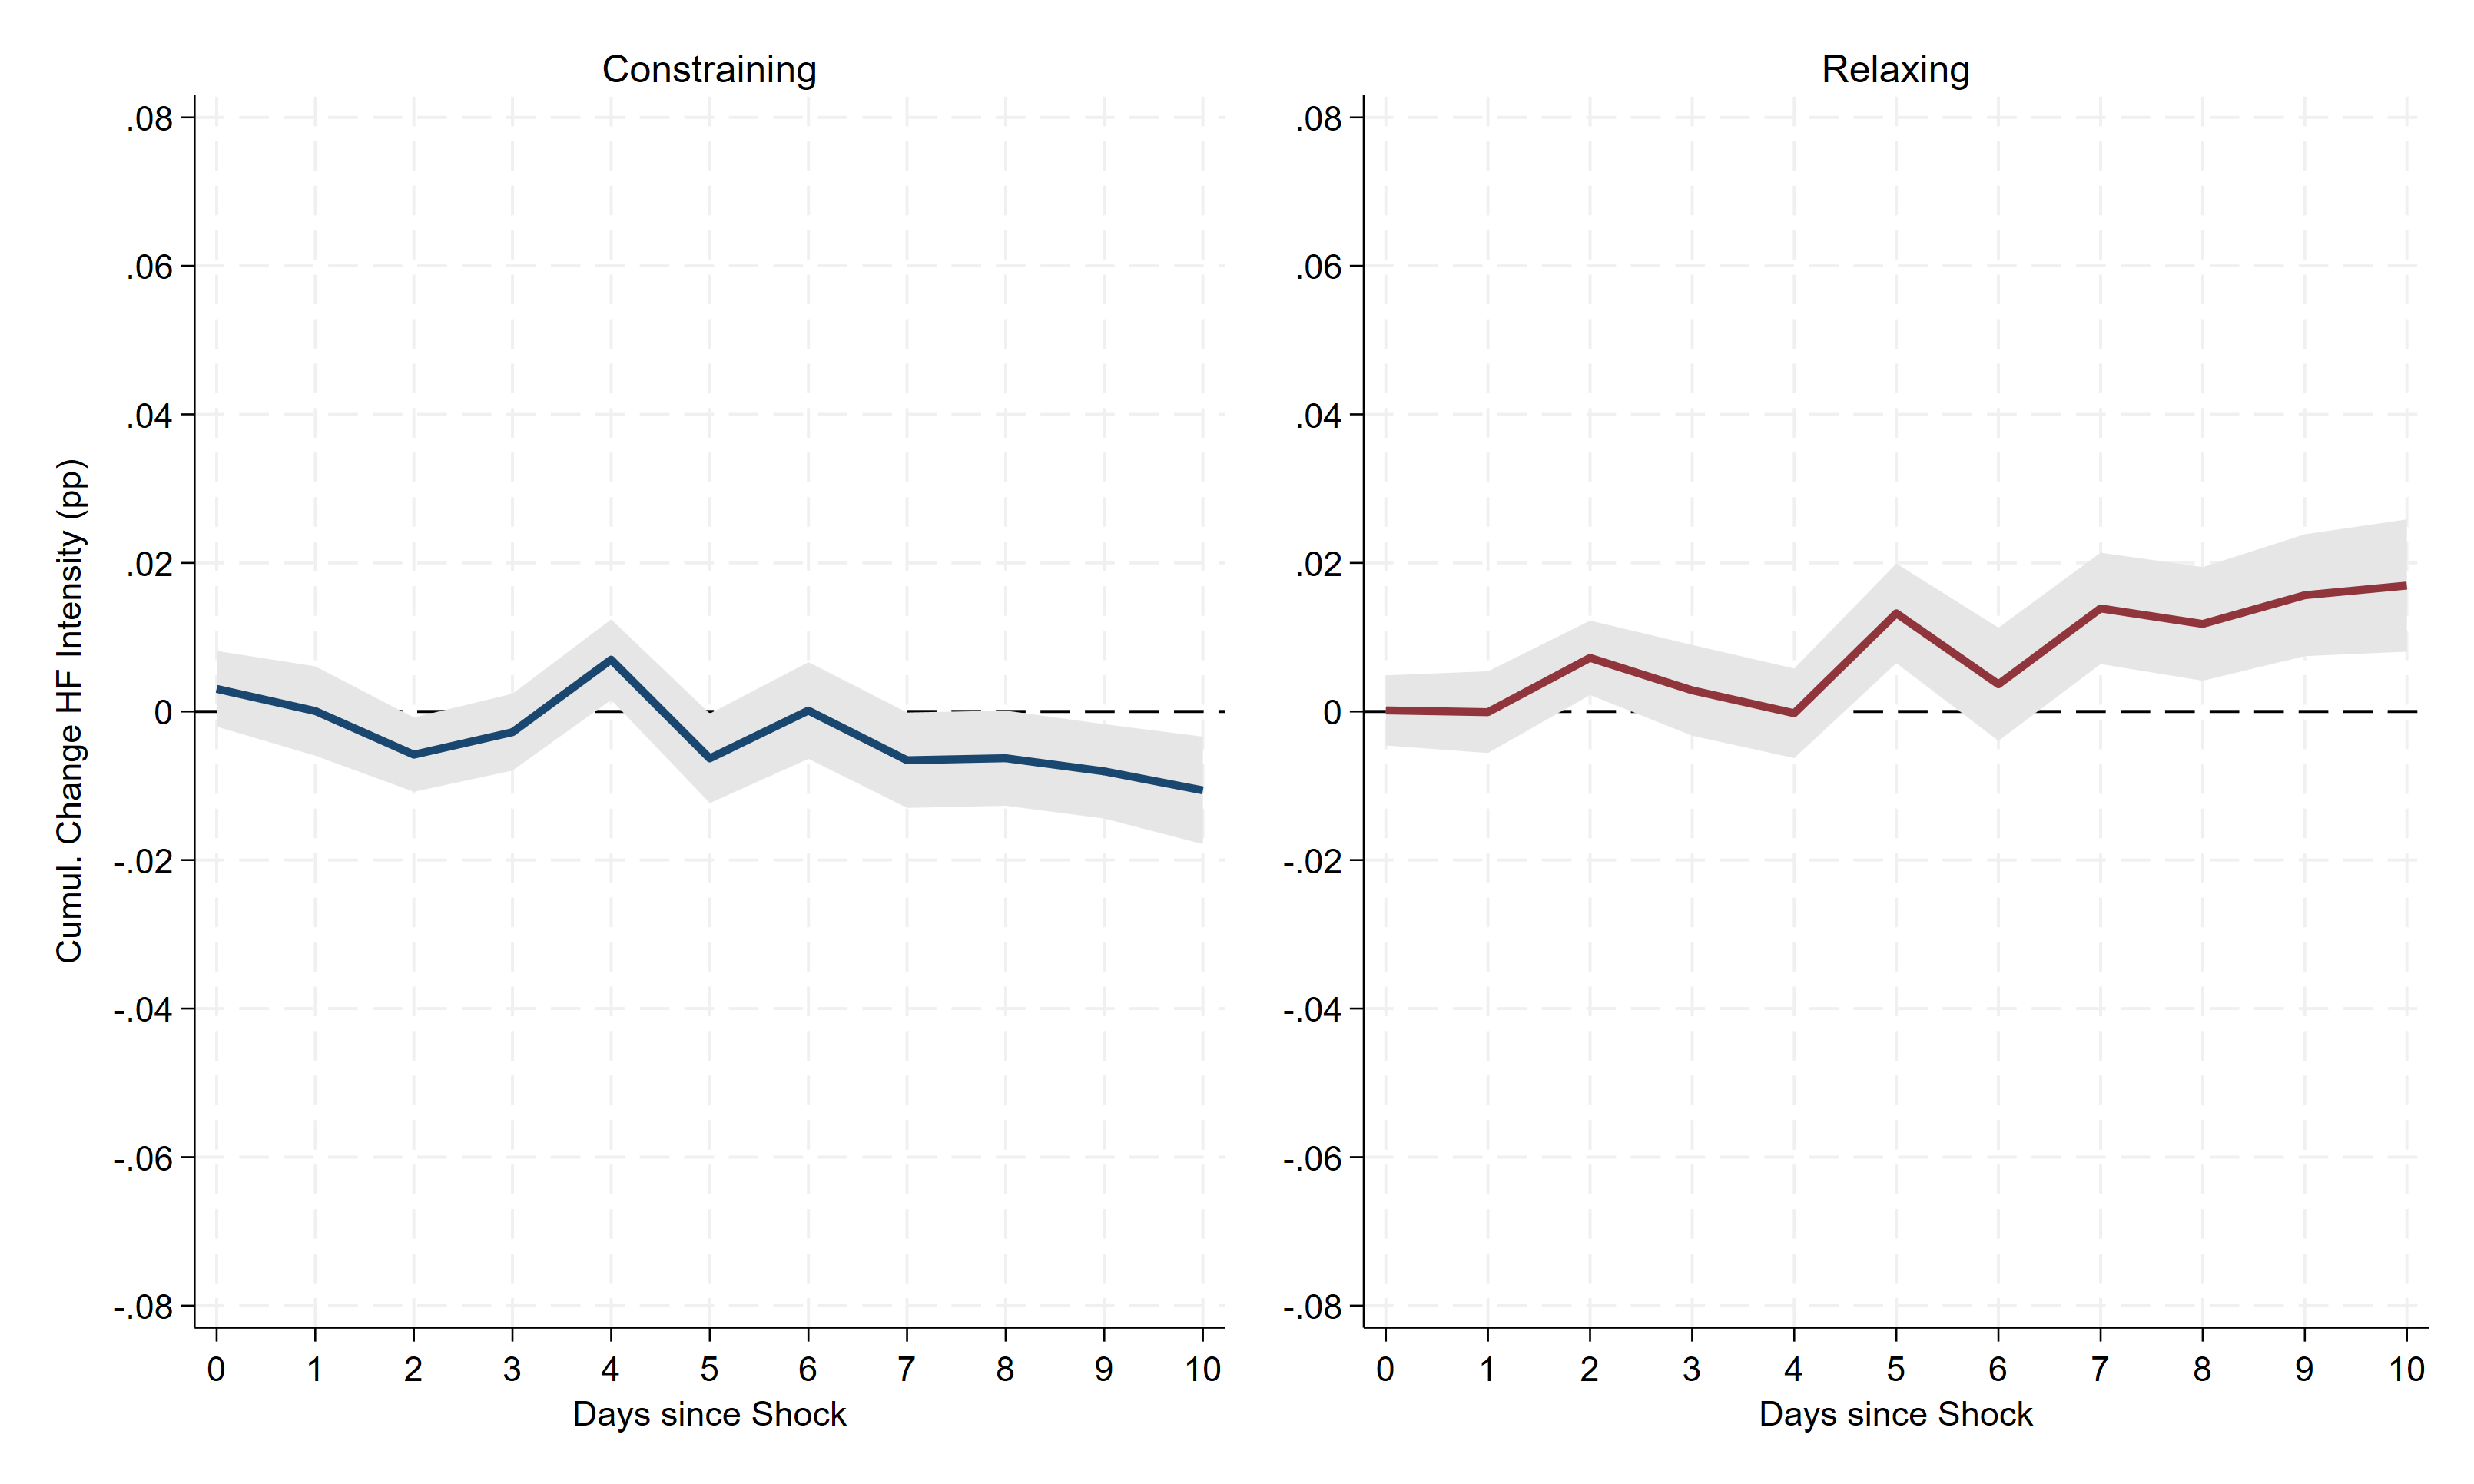
\includegraphics[width=\textwidth]{Figures/IR_term_momentum.png}
\vspace{-3mm}
% The note functions as the caption here
\caption*{\scriptsize \textit{Notes:} Dependent variable is the cumulative change in HF Intensity (pp) from $t-1$ to $t+h$. Intensity is measured as \% of amount issued. Sample restricted to term repo transactions. All specifications include bond fixed effects and duration $\times$ country $\times$ date fixed effects, with the latter absorbing the shock main effect. Identification of $\beta_h$ comes from within-cell variation in pre-shock positioning interacted with the shock. Standard errors clustered by date and bond. Shaded areas denote 90\% confidence intervals. \\ Sample period: 2021-01-01 -- 2025-11-01}
\label{fig:IR_term}
\end{figure}


\clearpage
\subsection{Excluding CTD bonds}
\label{subsec:ctd}

Table \ref{tab:no_ctd} re-estimates the main specifications on the subsample of non-CTD bonds to address the concern that unobserved futures exposure may transmit to cash yields through the cheapest-to-deliver linkage. Since CTD bonds are the primary instrument through which derivative positions affect underlying bond prices, amplification driven by off-balance-sheet futures exposure should be concentrated in this subset. The estimated coefficients are nearly identical to the main specifications across the binary, continuous intensity, constraining, and relaxing regime tests. This indicates that the amplification documented in the paper does not depend on the futures-cash linkage and reflects leveraged positioning observable through repo transactions. \\

\begin{table}[h!]
\centering
\caption{\textbf{Excluding CTD Bonds}}
\footnotesize
\setlength{\tabcolsep}{8pt}
\renewcommand{\arraystretch}{1.1}
\begin{tabular}{l c c c c}
\toprule
\textbf{Dependent Variable:} & \multicolumn{4}{c}{\textbf{$\Delta$ Bond Yield (bps)}} \\
\cmidrule(lr){2-5}
 & (1) & (2) & (3) & (4) \\
 & & & Constraining & Relaxing \\
\midrule
\textit{Main Interaction} & & & & \\
HF Involved $\times$ Shock & 0.281*** & & & \\
 & (0.061) & & & \\
Log HF Intensity $\times$ Shock & & 0.157*** & 0.132*** & 0.222*** \\
 & & (0.031) & (0.037) & (0.052) \\
\addlinespace
\textit{Direct Effects} & & & & \\
HF Involved & $-$0.020 & & & \\
 & (0.038) & & & \\
Log HF Intensity & & $-$0.013 & $-$0.018 & $-$0.010 \\
 & & (0.018) & (0.018) & (0.018) \\
\addlinespace
\textit{Controls} & & & & \\
Bid-Ask Spread & $-$0.265*** & $-$0.267*** & $-$0.264*** & $-$0.264*** \\
 & (0.076) & (0.076) & (0.075) & (0.075) \\
\midrule
Bond FE & Yes & Yes & Yes & Yes \\
Duration $\times$ Date $\times$ Country FE & Yes & Yes & Yes & Yes \\
\midrule
Observations & 455,303 & 455,303 & 451,642 & 451,598 \\
R-squared & 0.730 & 0.730 & 0.726 & 0.727 \\
\bottomrule
\end{tabular}
\label{tab:no_ctd}
\caption*{\textit{Notes:} This table re-estimates the main specifications on the subsample of non-CTD bonds. The dependent variable is the daily change in bond yield (bps). \textit{HF Involved} indicates the presence of offshore hedge fund repo activity. \textit{Log HF Intensity} is the natural log of one plus the average absolute hedge fund net position over the prior five trading days, scaled by the bond's total amount outstanding. Column (1) corresponds to Column (4) in Table \ref{tab:baseline}, Column (2) to Column (4) in Table \ref{tab:intensity}, and Columns (3) and (4) to Columns (1) and (2) in Table \ref{tab:asymmetry}. The Shock main effect is absorbed by the fixed effects. Standard errors are clustered by date and bond and reported in parentheses. *** p$<$0.01, ** p$<$0.05, * p$<$0.10. \\ Sample period: 2021-01-01 -- 2025-11-01}
\end{table}


\clearpage
\subsection{Exceedance probability CDS shocks}
\label{subsec:cds}

\begin{figure}[ht]
\centering
\caption{Probability of the Yield Change exceeding a Threshold by Day Type}
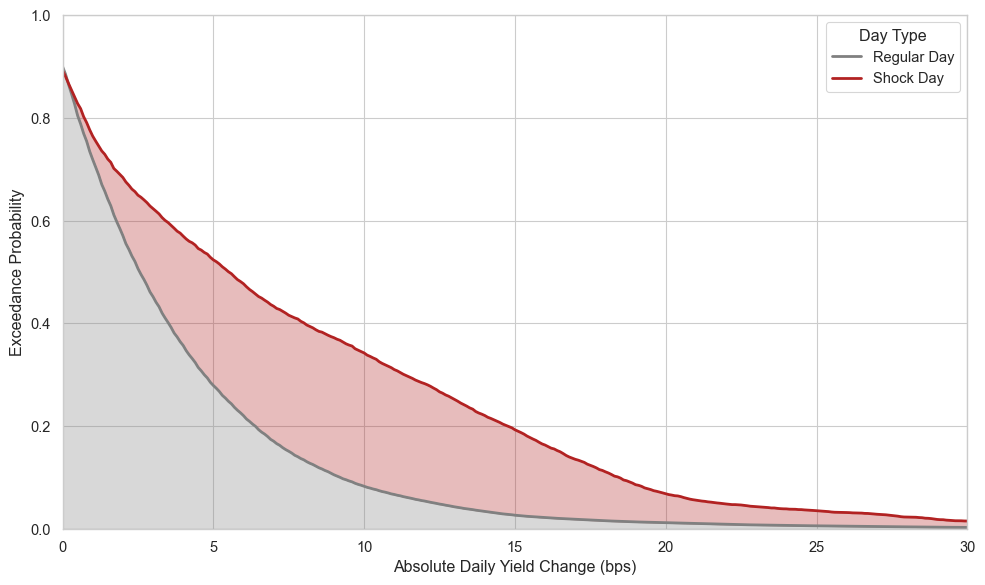
\includegraphics[width=\textwidth]{Figures/exceedance_probability_cds.png}
\caption*{\scriptsize \textit{Notes}: The figure plots the share of observations where the absolute daily yield change in Italian government bonds ($|\Delta y|$) is strictly larger than the threshold value displayed on the horizontal axis. The red line represents days with CDS shocks, while the gray line represents regular trading days. The shaded region between the curves highlights the excess tail risk generated by credit shocks. \\ Sample period: 2021-01-01 -- 2025-11-01}
\label{fig:exceedance_probability_cds}
\end{figure}



\clearpage
\subsection{Orthogonality of hedge fund positioning to the credit shock}
\label{subsec:orthogonality_cds}

Table \ref{tab:orthogonality_cds} repeats the orthogonality test of Section \ref{subsec:orthogonality} for the sovereign credit shock. It tests whether pre-existing hedge fund positioning is correlated with the realized credit shock through a common latent factor such as a shared macroeconomic outlook. As in the corresponding test for monetary surprises, the test is by construction based on the number of shock events in the sample, but the estimated relationship is economically negligible, explains essentially none of the variation in the shock, and is not statistically distinguishable from zero ($p = 0.77$). This supports the identifying assumption that pre-existing positioning is orthogonal to the realized credit shock.

\begin{table}[h!]
\centering
\caption{\textbf{Pre-existing Positioning and the Credit Shock}}
\footnotesize
\setlength{\tabcolsep}{8pt}
\renewcommand{\arraystretch}{1.1}
\begin{tabular}{l c}
\toprule
\textbf{Dependent Variable:} & \textbf{Credit Shock (bps)} \\
\midrule
 & (1) \\
\midrule
Lagged Aggregate HF Net Position & 0.034 \\
 & (0.118) \\
\addlinespace
Constant & $-$0.374 \\
 & (2.578) \\
\midrule
Observations & 38 \\
R-squared & 0.002 \\
\bottomrule
\end{tabular}
\label{tab:orthogonality_cds}
\caption*{\textit{Notes:} This table reports the orthogonality test of hedge fund positioning against the realized credit shock. The dependent variable is the residualized change in the five-year US dollar Italian sovereign CDS spread on credit shock days. \textit{Lagged Aggregate HF Net Position} is the sum of Cayman-domiciled hedge fund net repo positions across all bonds on the trading day before each credit shock. Robust standard errors are reported in parentheses. \\ Sample period: 2021-01-01 -- 2025-11-01}
\end{table}




\end{document}

